\documentclass[11pt]{amsart}
\usepackage{geometry}                % See geometry.pdf to learn the layout options. There are lots.
\geometry{letterpaper}                   % ... or a4paper or a5paper or ... 
%\geometry{landscape}                % Activate for for rotated page geometry
%\usepackage[parfill]{parskip}    % Activate to begin paragraphs with an empty line rather than an indent
\usepackage{graphicx}
\usepackage{amssymb}
\usepackage{url}
\usepackage{epstopdf}
\usepackage{amsmath}
\usepackage{tikz}
\usepackage{subcaption}
\usepackage{bm}
\usepackage{setspace} 
\doublespacing
\DeclareGraphicsRule{.tif}{png}{.png}{`convert #1 `dirname #1`/`basename #1 .tif`.png}
\usetikzlibrary{arrows,positioning}
% LB things
\newenvironment{packed_item}{
\begin{itemize}
 \setlength{\itemsep}{0pt}
  \setlength{\parskip}{0pt}
  \setlength{\parsep}{0pt}
}{\end{itemize}}

\newcommand{\Unif}{\text{Unif}}
\newcommand{\Beta}{\text{Beta}}
\newcommand{\Normal}{\text{Normal}}
\newcommand{\Binomial}{\text{Binomial}}
\newcommand{\E}{\mathbb{E}}
 
 



\title{Mechanistic Bayesian Forecasts of COVID19}
\author{Graham C. Gibson, Nicholas G. Reich, Daniel Sheldon}
%\date{}                                           % Activate to display a given date or no date


\begin{document}
\tableofcontents


\maketitle

\section*{Abstract}

The COVID-19 pandemic emerged in late December 2019. In the first six months of the global outbreak, the US reported more cases and deaths than any other country in the world. Effective modeling of the course of the pandemic can help assist with public health resource planning, intervention efforts, and vaccine clinical trials. However, building applied forecasting models presents unique challenges during a pandemic. First, data quality suffers from under-reporting, delayed reporting due to reporting infrastructure issues, and limited testing. Second, interventions are time-varying across different geographies leading to large changes in transmissibility over the course of the pandemic. Finally, the unidentifiability of the epidemiological parameters leads to difficulty in model fitting. We propose a novel Bayesian compartmental model (MechBayes) that builds upon the classic compartmental framework of susceptible-exposed-infected-recovered (SEIR) model to operationalize COVID-19 forecasting in real time. This includes non-parametric modeling of varying transmission rates, non-parametric modeling of case and death discrepancies due to testing and reporting issues, and finally joint observation likelihood on new case counts and new deaths. The model has been used to submit forecasts to the US Centers for Disease Control, through the COVID-19 ForecastHub \cite{covidhub}.  We examine the performance relative to a baseline model in addition to performing an ablation test of our extensions to the classic SEIR models. We demonstrate a significant gain in both point and probabilistic forecast scoring measures using MechBayes.
%\begin{itemize}
%\item Covid has affected XX people
%\item Forecasts useful for public health resource planning, intervention planning (vaccine trials), and disease burden
%\item Basic Mechanistic Models unable to capture complexities of real world disease epidemics due to 
%\begin{itemize}
%\item Complexities of interventions 
%\item Issues with testing and reporting
%\end{itemize}
%\item We propose a novel forecasting algorithm to overcome 
%\begin{itemize}
%\item Under-reporting of cases
%\item Time-varying interventions
%\end{itemize}
%\item Bayesian end to end estimation using both cases and deaths in numpyro
%\end{itemize}



%\section{}
%\subsection{}

\section{Introduction}

The emergence of COVID-19 in early 2020 in the United States led to the largest pandemic in over a century. Understanding the future trajectory of the impact in terms of healthcare burden, economic, treatments and public health response. Forecasts of incident and cumulative deaths due to COVID-19 help in resource allocation, vaccine clinical trial planning, and re-opening strategies \cite{ray2020ensemble}. Forecasts provide important data to decision-makers and the general public and can improve situational awareness of current trends and how they will continue in coming weeks. 

Infectious disease forecasting, at the time horizon of up to 4 weeks in the future, has benefited public health decision makers during annual influenza outbreaks \cite{lutz2019applying,myers2000forecasting}.  However, many forecasts of seasonal disease, such as influenza, often rely on ample historical data to look for patterns that can be projected forward into the future. In an emerging pandemic situation, models must be able to fit to limited data. 

In modeling the COVID-19 pandemic, many research groups have turned to the use of compartmental models to explain the underlying transmission of a disease through a population. First introduced by  Kermack and McKendrick, such models assume the each individual is in one of a mutually exclusive set of compartments, typically either the susceptible, exposed, infected, or recovered compartment \cite{kermack1927contribution}. A model is specified by setting the rates of flow of individuals between compartments. While these models have been used since their inception in the early 20th century, the COVID pandemic represents a unique opportunity to explore their forecasting properties in real-time at both local and global scales.
 
 
 Our main goal in developing MechBayes is to forecast observed incident deaths, and because we have limited historical data on COVID-19, we think compartmental models are among the most parsimonious models available for forecasting. Our focus is not on inference but forecasting. Therefore, identifying internal parameters of the model, many of which are poorly determined or not identifiable from the available data. We distinguish this from scenario projection models, which require well identified epidemiological parameters that can be set to counterfactual values under different scenarios, such as an increase or decrease in intervention levels. These models, however, are often not flexible enough for real-time forecasting. 
 
We introduce a novel operational forecast model based on mechanistic foundations and tailored to the particular needs and data availability of COVID-19. These include, but are not limited to, severe under reporting of cases due to low testing rates especially in mild or asymptomatic cases, time-varying testing rates, delayed reporting, and both the addition and removal of control measures such as social distancing, lockdown, and mask use. We accomplish this by modeling transmission and deviations from cases and deaths (beyond the case fatality ratio) non-parametrically.  We choose a Bayesian framework that allows for uncertainty in the epidemiological parameters that are unidentifiable from the data, introducing flexibility suited to forecasting. Implementation in a Bayesian framework also allows for use of a cutting edge probabilistic programming framework for computational speed. 


 We demonstrate the success of the model in both forecast submissions to the US Centers for Disease Control via the COVID-19 Forecast Hub as well as an ablation model comparison to demonstrate the additional forecast accuracy of our extensions beyond the basic SEIR model. In what follows we first describe the available data and forecast submission infrastructure, outline the basic SEIR compartment model, describe our extensions for real-world pandemic forecasting, and finally evaluate the model using both real-time evaluation from submissions and a retrospective model component analysis. 



\section{Related Work}

Compartmental models have been used to effectively model and forecast disease in non-pandemic situations both retrospectively and in real-time. These include complex compartmental models for real-time influenza forecasting \cite{shaman2012forecasting, osthus2017forecasting,ong2010real}, and a retrospective model evaluation of the 1918 influenza pandemic \cite{hall2007real}. Compartmental models have been used not just in respiratory disease but in Ebola \cite{lekone2006statistical}, measles \cite{bokler1993chaos}, dengue \cite{syafruddin2012seir} and a wide variety of other diseases

Compartmental models have also been adopted into a Bayesian framework before, including both stochastic disease dynamics and deterministic dynamics \cite{hotta2010bayesian,dukic2012tracking}. Non-parametric transmissibility was included in a Bayesian SEIR model to study Ebola by Frasso and Lambert \cite{frasso2016bayesian}. Time-varying transmissibility has also been studied in the frequentist setting using complex non-parametric functions \cite{smirnova2019forecasting}. Many efforts have been made to use SEIR models in forecasting COVID-19 \cite{giordano2020modelling,yang2020modified,bertozzi2020challenges}\cite{prem2020effect,flaxman2020estimating}. With the outbreak of COVID-19, accounting for testing has become a critical element in effectively using an SEIR model  \cite{lopez2020modified,pei2020differential}. 


%*Models that have accounted for time-varying testing have mostly used the renewal style equations \cite{abbott2020estimating}\cite{flaxman2020estimating}. 
%These models do not use a differential equation model as the core component, but rather parameterizes new cases as a function of the time varying reproduction number and the serial interval. 

\section{Model Overview}

MechBayes extends the SEIR model framework to account for a joint observation model on incident cases and deaths, time-varying transmission, and time-varying discrepancies in the case fatality ratio due to testing, asymptomatic cases etc. We do this by choosing flexible non-parametric models that capture trends in disease parameters without relying on external data. 

\section{Data}
	In this analysis we used confirmed case counts and deaths as reported by the Johns Hopkins University Center for Systems Science and Engineering \cite{dong2020interactive}. This a time series dataset which we truncate to begin March 1st 2020 to August 1st 2020 and captures all 50 states, as well as Guam, Puerto Rico, American Samoa, District of Columbia, Northern Mariana Islands and U.S. Virgin Islands. As noted in \cite{krantz2020level}, COVID-19 cases are under-reported, with the fraction of all infections reported as cases for the U.S. estimated at 20-30\% \cite{russel2020using}. 
	
	
		%There are large discrepancies in reporting practices across the states (Figure \ref{fig:data}). For example, New Jersey reported an additional 1600 incident deaths when changing reporting practices to include ``probable" deaths as well as confirmed deaths due to COVID-19 on June 25th 2020. However, many other states have at least one outlying value, usually due to delayed reporting, where a large number of deaths occurring in previous weeks are reported on a single day. We can also see from Figure \ref{fig:data} that some states do not report on particular days (usually weekends) leading to 0 incident deaths for the day. Some states also revise the cause of death, allowing for negative incident deaths.  Some states exhibit relatively regular weekly reporting cycles, with reporting dropping off significantly on the weekends. This effect is most pronounced at the aggregate U.S. level, which shows a clear weekly cycle in reporting. 
	
\section{Targets}	
We made probabilistic forecasts  for 1--4 week ahead incident and cumulative deaths for all geographies. An individual forecast distribution is represented by a set of quantiles, $\mathbb{Q} = {.01,.05,.10,....,.90,.95,.99}$, with the median ($.5$ quantile) representing the point-forecast. Since our model produced cumulative forecasts by aggregating incident, we choose to only evaluate incident. 

%Forecasts were made on Monday evenings and therefore use the incident data up until the Sunday before. A one-week ahead target corresponds to the following Saturday. A two-week ahead corresponds two the next Saturday and so on. Forecasts were evaluated using mean-absolute-error (MAE) and empirical coverage probability at the 95\% level. This allows us to assses both point prediction and calibration of forecasts.



 \begin{figure}
     \centering
     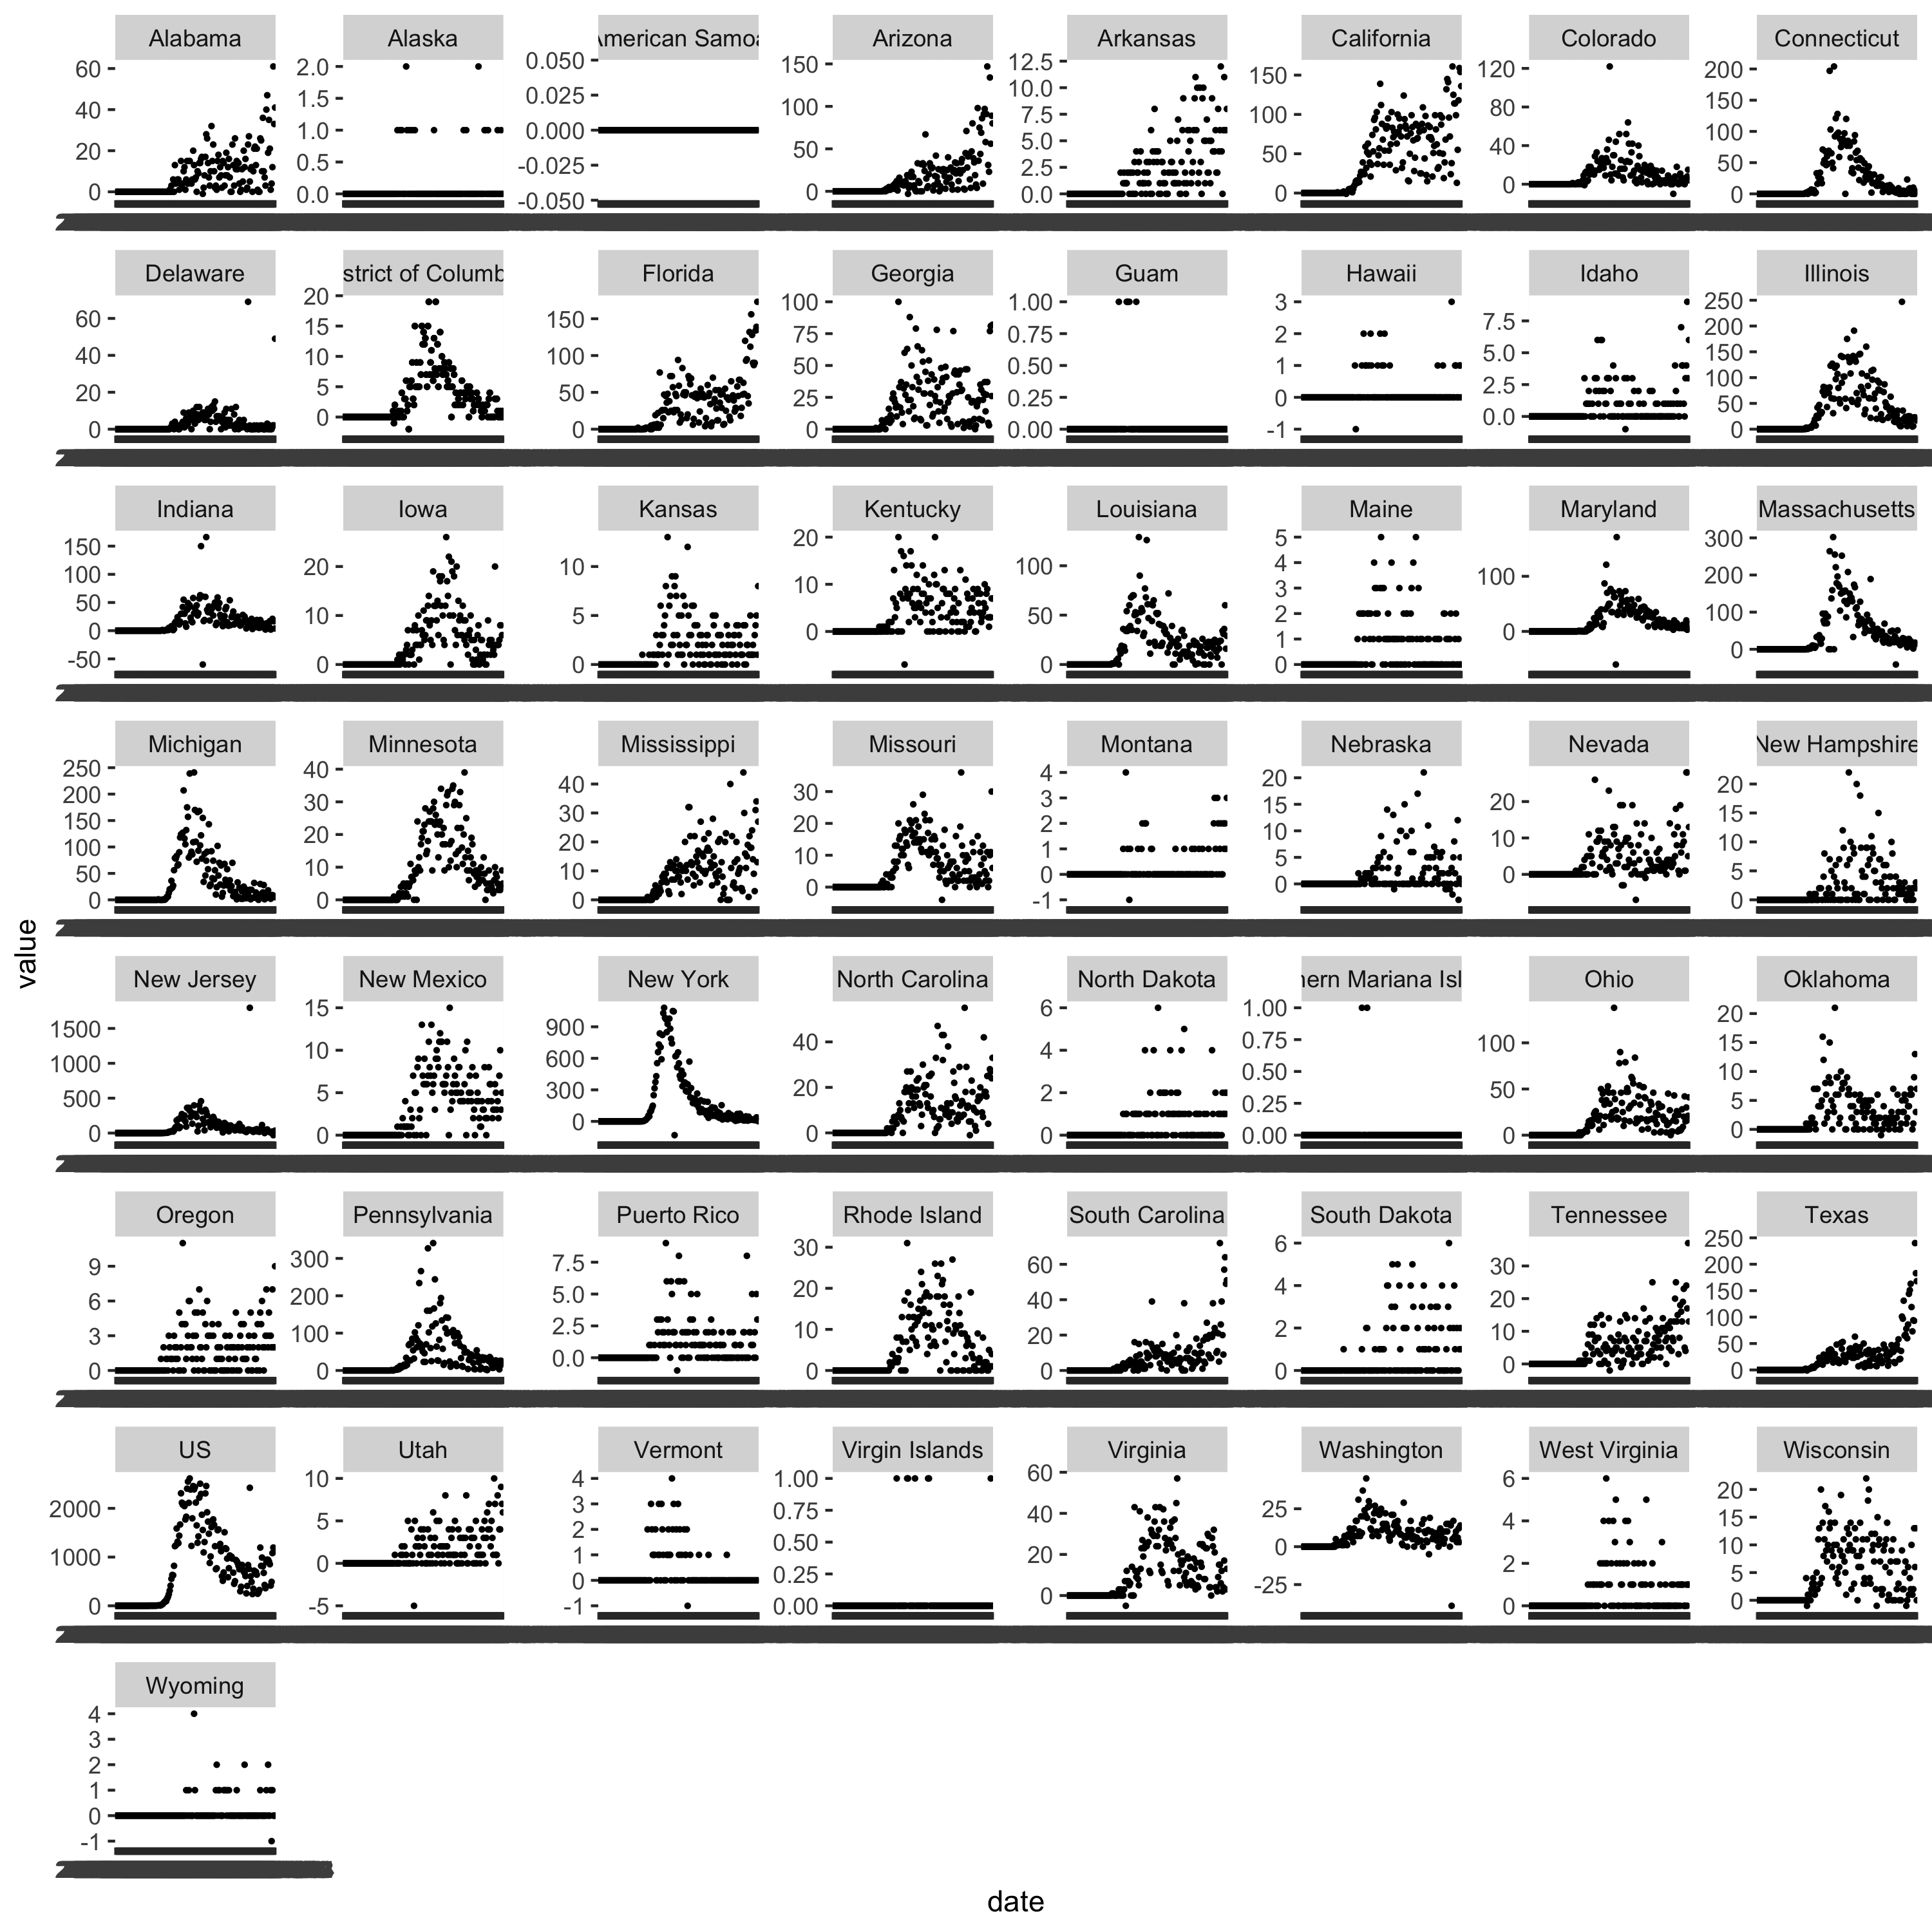
\includegraphics[scale=.17]{data_plot.png}
     \caption{Deaths by state for any state with over 50 incident deaths for a given day. Notice the large variability in incident reporting. There are significant delayed reporting, with New Jersey reporting over 1500 backlogged deaths when switching to include ``probable" deaths. In some states, there appears to be a weekly cycle where deaths are under-reported on the weekend. This is especially pronounced for the U.S. as a whole. We can also see that there are some negative incident deaths, where data are revised to account for deaths that were incorrectly attributed to COVID-19. }
     \label{fig:data}
 \end{figure}
 
 \section{MechBayes}

In a given time-step (e.g. one day), each member of the population of a single geography belongs to one of the following mutually exhaustive compartments:
 susceptible $S$, exposed but not yet infectious $E$, infectious $I$, recovered $R$, hospitalized before death $D_1$, and deceased $D_2$ (Figure \ref{fig:seird}). Here we assume everyone who is hospitalized will eventually become deceased in order to separate the rate of flow into both a case fatality ratio (CFR) parameter as well as a time from symptoms to death parameter, which both have prior estimates from the literature \cite{russell2020estimating}. We omit an explicit hospitalization compartment since the available hospitalization data is highly variable by state and suffers even more reporting issues than case data.  For simplicity, we assume a closed population of size $N$. 
The following parameters govern how members of the population move between compartments:  
\begin{packed_item}
\item $\beta(t)$: transmission rate, which we allow to vary by time $t$
\item $\sigma$: rate of transition from the exposed state $E$ to infectious state $I$; i.e., $1/\sigma$ is the expected duration of the time between exposure and symptom onset. 
\item $\gamma$: rate of transition from  the infectious state $I$ to no longer being infectious (either to state $D_1$ or $R$); i.e., $1/\gamma$ is the expected duration of the infectious period
\item $\rho$: fatality rate (i.e., probability of transitioning from I to $D_1$ instead of I to R)
\item $\lambda$: rate of transition from $D_1$ to $D_2$ 
(i.e., the inverse of expected number of days in $D_1$ compartment before death) 
\end{packed_item}
For a given time-step $t$, the following differential equations describe the changes in each compartment:

\begin{equation}
\begin{aligned} 
\frac{dS}{dt} &= - \beta(t) \frac{SI}{N} \\
\frac{dE}{dt} &= \beta(t) \cdot \frac{SI}{N} - \sigma E \\
\frac{dI}{dt} &= \sigma E - \gamma I\\ 
\frac{dR}{dt} &= (1-\rho)\gamma I \\
\frac{dD_1}{dt} &= \rho \gamma I - \lambda D_1\\
\frac{dD_2}{dt} &= \lambda D_2\\
\frac{dC}{d} &= \sigma E
\end{aligned}
\end{equation}

Here, we include the $C$ compartment to be able to observe the cumulative count of new infections. This captures only the flow into $I$.

We can write this in a state space representation as follows: \[
X(t) = (S(t), E(t), I(t), R(t), D_1(t), D_2(t), C(t))
\]
The update from time $t$ to time $t+1$ can be solved numerically as
\begin{equation}
\bm{X}(t+1)= \text{RK4}\left(\bm{X}(t),\frac{dX}{dt},\beta(t)\right)
\end{equation},
where RK4 is the Runge-Katta 4th order approximation \cite{phan2019composable}.


\begin{figure}
 \begin{center}
\begin{tikzpicture}[node distance=1cm,auto,>=latex',every node/.append style={align=center},int/.style={draw, minimum size=1cm}]
    \node [int] (S)             {$S$};
      \node [int,right=of S] (E)  {$E$};
    \node [int, right=of E] (I) {$I$};
        \node [int, above=of E] (C) {$C$};

    \node [int, right=of I] (D_1) {$D_1$};
    
    \node [int, right=of D_1] (D_2) {$D_2$};
     \node [int, below=of I] (R) {$R$};

   % \coordinate[right=of ] (out); %
    \path[->, auto=false] (S) edge node[yshift=12pt] {$\beta(t) I$ \\[.2em]} (E)
                          (E) edge node[yshift=5pt] {$\sigma$       \\[.2em] } (I) 
                           (E) edge node[yshift=-12pt,xshift=5pt] {$\sigma$       \\[.2em] } (C) 
                           (I) edge node[yshift=5pt] {$\rho\gamma$       \\[.2em] } (D_1)
                           (I) edge node[xshift=30pt,yshift=-5pt] {$(1-\rho)\gamma$       \\[.4em] } (R)
                            (D_1) edge node[yshift=5pt] {$\lambda$       \\[.2em] } (D_2)  ;
                          \end{tikzpicture}
\end{center}
      \caption{Comparmental model parameters }
     \label{fig:seird}
 \end{figure}
 
 
 
 

 
 \subsection{Time-varying transmission}
 
We have seen significant efforts to control the spread of COVID through non-pharmaceutical interventions. These include social distancing, lock-downs, and mask wearing. To add to the complexity, these interventions have been implemented and repealed at different time points. They also face compliance issues \cite{simonov2020persuasive}. In order to capture the aggregate effect of the interventions non-parametrically we choose a flexible model for the time-varying transmission parameter.
We allow $\beta(t)$ to vary as follows, 

\begin{equation}
log(\beta(t)) \sim N(log(\beta(t-1)), \sigma_{\beta}^2)
\end{equation}

This model assumes that forecasts are made on the current level of interventions because $\mathbb{E}[log(\beta(t+1))] = log(\beta(t))$. That is, the expected value of a random walk in the forecasting stage is the estimated value at the final time point of available data.

However, this non-parametric model is particularly susceptible to noise in reporting of cases, since $\beta(t)$ is the parameter that takes individuals from $S$ into $E$. To avoid instability issues, especially when forecasting, we smooth each posterior sample of $\beta$ to be the average over the last 10 days from the sample. This is a large enough window to smooth over most reporting issues (excepting delayed reporting). 

\begin{equation}
\beta^*_{forecast}(t+k) = \frac{1}{10}\sum_{i=0}^{9}\beta^*(t-i)
\end{equation}

where $\beta^*(t)$ denotes a sample from the posterior at time $t$.

% \begin{itemize}
% \item Non-parametrically models time-varying transmissibility through a random walk
% \item Makes forecasts conditional on current level of interventions
% \item Requires no external intervention data to make forecasts 
% \end{itemize}
% 
 \subsection{Observation Model}
 
 The observed data used to fit the model is based on time-series data of incident confirmed cases $Cases_{t}$ and incident recorded deaths $Deaths_{t}$. 
For a given state and day, the change in the  confirmed cases and reported deaths are subset of the cumulative number of new infections $C(t)$ and cumulative number of deaths $D2(t)$, respectively. To handle this, we introduce two additional parameters. First, we introduce a case and death deviation, beyond the case fatality ration, of cases $p_{c,t}$ and the case and death deviation model of deaths $p_d$. For both, we set fairly flat priors to reflect these parameters are poorly determined from observed data.

In more detail, $p_{c,t}$ can be thought of as an aggregate probability of a case being detected and then flowing through the compartments. We assume its prior distribution is given by  $p \sim \Beta(15, 35)$, such that  $\E[p_c] = 0.3$  with 90\% probability between $0.22,0.38$. This means that we expect 30\% of cases to be detected initially, as suggested by the literature \cite{midas}. However, we also allow this to vary by time. We do not intend for this to be interpretable as purely reflecting testing, but rather an aggregate measure of testing, reporting issues, and general departure from our prior estimate of the case fatality ratio.

\begin{equation}
logit(p_{c,t}) \sim N(logit(p_{c,t-1}), \sigma^2)
\end{equation}

We also assume the probability that a COVID-19 death is reported $p_d$ has a prior distribution given by  $p_d \sim \Beta(90, 10)$. This prior satisfies $\E[p_d] = 0.9$ with 90\% probability between 0.89,0.92. That is, we assume that deaths due to COVID-19 are most often correctly reported \cite{weinberger2020estimation}. 

 


Using the above SEIR model and these detection probabilities, we can then express the observed incident numbers of confirmed cases and deaths as follows.
\begin{equation}
\text{Cases}_{t} \sim NB(p_{c,t}*[C_{t} - C_{t-1}],\sigma_{c}^2)
\end{equation}

\begin{equation}
\text{Deaths}_{t} \sim NB(p_d*[D_{2_{t}} - D_{2_{t-1}}], \sigma_d^2)
\end{equation}

Where the difference in $C_{t}-C_{t-1}$ allows us to translate cumulative new cases to incident cases and similarly with deaths. 
%  \begin{itemize}
% \item Non-parametrically models time varying testing and overall detection of case issues
% \item Allows for "data dumps"
% \item Logistic random walk 
% \item Fixed case and death deviation model on deaths
%
%  \end{itemize}

\subsection{Epidemiological Model Parameters}

We use relatively informative priors for epidemiological parameters, such as $\gamma$, $\sigma$, $\rho$,  $\lambda$, and initial compartment values. The details are described in the Appendix A1. However, the identifiability of model parameters in compartmental models where the data consists only of a time series of incident cases and deaths presents a problem for uninformative priors. Using the renewal style equations, it can be shown that the number of newly infected at time $t$ is a function of the time-varying reproductive number, serial interval and previously reported new infections \cite{wallinga2007generation}. This means that a single time series does not contain enough information to separately estimate both the serial interval and the time-varying reproduction number. In an SEIR model, the serial interval is distributed exponential with rate parameter $\sigma + \gamma$ \cite{wallinga2007generation}. Additionally, the time varying reproduction number is $R_t = \frac{\beta(t)*S(t)}{\gamma}$. Therefore, the time series of incident cases is not enough to uniquely identify $\gamma,\sigma,\beta(t)$. In order to make the model identifiable, we impose tight priors on the parameters $\sigma$ and $\gamma$ as estimated by the literature (in essence fixing the serial interval), and we let $\beta(t)$ vary freely. This reflects the underlying biology of the system, since the reciprocal of the sum of $\sigma$ and $\gamma$ may be interpreted as the average time from when an individual becomes infected to when they infect someone else, given that they infect someone else. This is a biological property of the disease, rather than $\beta(t)$ which contains both the biological transmissibility as well as the aggregate effects of human behavior through intervention. This highlights a fundamental philosophical difference between using compartmental models for forecasting rather than interpreting parameters for epidemiological purposes. However, putting relatively informative priors on $\sigma$ and $\gamma$, instead of fixing them, still allows for variation by state due to differing demographic characteristics such as age structure. Fitting the model in a Bayesian way allows for this unique trade off.  

  \subsection{Fitting}
We use the Hamiltonian Monte Carlo algorithm implemented in numpyro to fit the model to data \cite{numpyro}. That is, given a time series of confirmed cases ($\text{Cases}_{1:t}$) and confirmed deaths ($\text{Deaths}_{1:t}$) we use Bayesian inference (via HMC) to obtain 

\begin{equation}
f(\bm{\theta} | \text{Cases}_{1:t},D_{1:t}) \propto f(\text{Cases}_{1:t},\text{Deaths}_{1:t} | \bm{\theta})f(\bm{\theta})
\end{equation}
where $\bm{\theta}$ is a vector containing all model parameters. 

\begin{equation}
\bm{\theta} =[\beta_{t} ,
\sigma ,
\gamma ,
\rho ,
\lambda ,
p_{c,t} ,
p_{d} ,
\sigma_c^2 ,
\sigma_d^2 ,
I_0 ,
E_0 ,
D_{1_0} ,
D_{2_0} ,
R_0 ]
\end{equation}

We draw 1000 warm-up sample and then 1000 posterior samples of model parameters. This allows us to forecast using the posterior predictive distribution.

\begin{equation}
f(C_{t:(t+h)}, D_{t:(t+h)}) =  \int_{\theta} f(C_{1:t},D_{1:t} | \bm{\theta})f(\bm{\theta})
\end{equation}

\textbf{For dan to fill in}
 \section{Experimental Setup}
 To evaluate our model, we examine two different scenarios. First, we describe the submission process and infrastructure used for the real time evaluation as part of the U.S. Centers for Disease Control (CDC) COVID-19 Forecast Hub consortium. Second, we describe the internal evaluation used to demonstrate our model enhancements improve accuracy over a naive compartmental model. 
 
 \subsection{CDC Forecast Evaluation}
We began submitting forecasts to the CDC for incident deaths on May 10th 2020 and have since submitted forecasts every Monday from then until August 1st 2020. The forecasts use daily data up to and including the Sunday before submission the next Monday. The one week ahead forecast corresponds to the following Saturday, the two week ahead to the second following Saturday and so on.  We use the model submissions made in real-time evaluated on both MAE and coverage probability for 13 submissions. We subset to the 50 states and Washington D.C., which is the largest set of locations where forecasts were made for each date. 
 
 In the real-time evaluation we also made manual adjustments to account for delayed reporting through a quality-assurance process. This involved,
 
 \begin{itemize}
 \item Identifying outliers in recently reported incident cases.
 \item Searching for documented evidence of a data dump. These are usually recorded on state department of health websites and sometimes local news outlets.
 \item Manually redistributing the incident deaths evenly over the time-frame mentioned by the department of health or news outlet for the backlog window.
 \end{itemize}
 
 
 This process ensured that the observed data does not contain any identifiable outliers (meaning documented by outside sources). In real-time this is necessary to avoid drastic over-predictions caused by delayed reporting. For example, New Jersey reported nearly 1,600 daily deaths as it switched from reporting only confirmed deaths from COVID-19, to confirmed and probable on 2020-06-25. This would have caused a drastic increase in predictions if not properly identified as data dump. On 2020-07-07 Texas removed 3,000 confirmed cases when they discovered the reported cases were a result of anitgen testing, which were not considered reportable. 
% \begin{itemize}
% \item Real-time forecasting evaluation for 14 weeks starting April 20th 2020. 
% \item Forecasts submitted every Monday using incident data up until Sunday
% \item Cumulative forecasts generated by aggregation of incident forecasts
% \item 1-4 week ahead targets generated from 28 day ahead predictions 
% \end{itemize}
 
 We compare the results against the CDC baseline model. This is a purely statistical model that uses historical COVID-19 deaths only. At all forecast horizons, the median of the forecast distribution from the baseline model is equal to the most recent reported incidence. The model obtains a non-parametric distribution around this median by adding and subtracting past observed differences in incidence from one week to the next for a specific location. This model is fit state by state. 
   
 
 \subsection{Ablation Test}
 
 While real-time model evaluation is valuable for understanding evolving model performance, we also perform a retrospective evaluation using three model variants to demonstrate the improvement in accuracy over a baseline SEIR model. We define the following variations on MechBayes,
 
 \begin{itemize}
 \item \textbf{MechBayes Case/Death Time-Varying} Mech Bayes as submitted to the CDC. That is, a model using negative binomial observation noise as well as a time-varying random walk, using a joint likelihood over cases and deaths.
 
 \item \textbf{MechBayes Case/Death Fixed} MechBayes Case/Death Time-Varying with $p_{c,t}$ fixed to $p_c$, that is, removing the time-varying case and death deviation model.
 
 \item \textbf{MechBayes Death Fixed} MechBayes Case/Death Time-Varying with observations on cases removed.
 \end{itemize}
 
 Note that these are nested models, with MechBayes Death Fixed contained in MechBayes Case/Death Fixed contained in MechBayes Case/Death Time-Varying. 
 
  
 We also fix all non-model component variation. That is, we average over the last 10 days of $\beta(t)$ when forecasting, as well as manually redistributing delayed reporting. This ensures that the comparison is only on model components, and not on data discrepancies. Note that we do not include a model without a time varying transmissibility parameter. This is because such a model would assume no interventions were put in place, which clearly violates the data-generating process. Previous Covid-19 modeling attempts have established that time-varying transmissibility is essential \cite{pei2020differential,abbott2020estimating,flaxman2020estimating,smirnova2019forecasting}.



\begin{figure}

    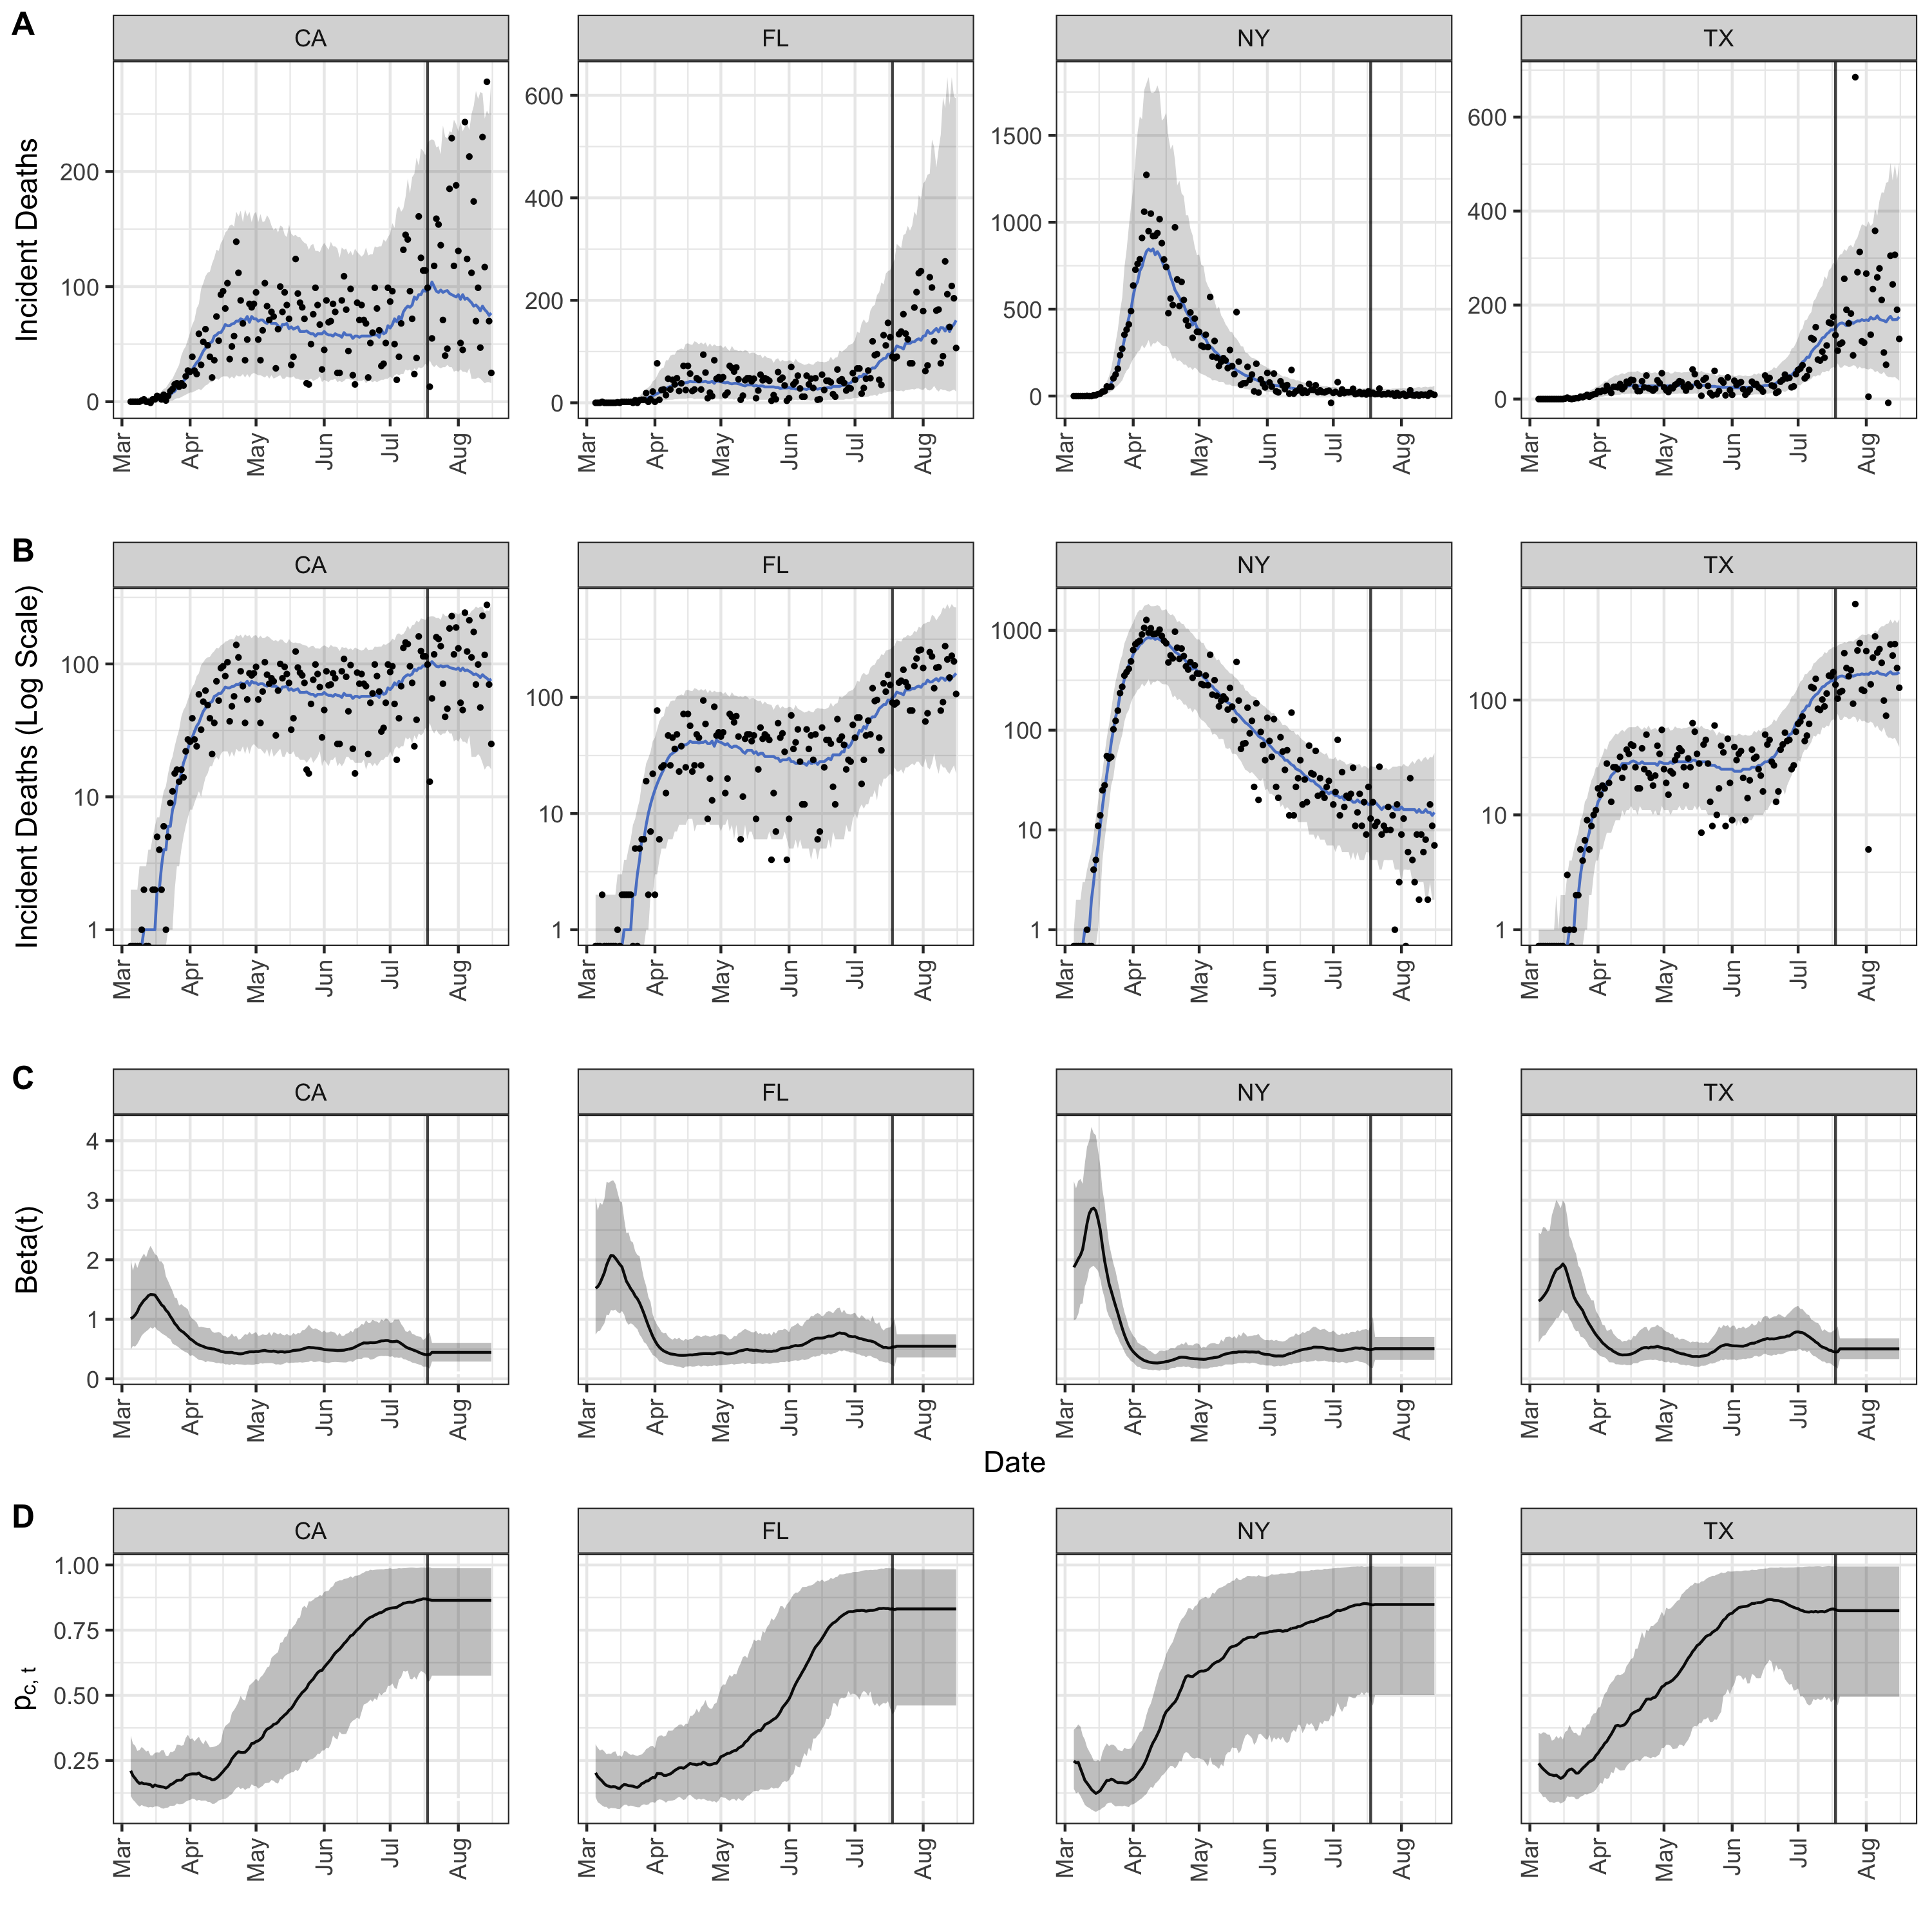
\includegraphics[scale=.15]{fig3.png}

\caption{\textbf{A,B} Example fit and forecast for 2020-07-19 for four selected states. Grey bands represent 95\% prediction intervals. Blue line represents median forecast. MechBayes is able to produce well calibrated fits to the data as well as accurately tracking trends in incident deaths. \textbf{B} Posterior of $\beta_t$ for each of the four states, with 95\% credible intervals in blue. Note that this parameter does not reflect interventions specifically, but rather any change in transmissibility. \textbf{C} Posterior of the case-death discrepancy for the four example states. Here we can see that over time, the number of observed cases that resulted in deaths increased. This does not necessarily reflect testing, but an overall increase in the ability to observe cases as compared to the predicted number of cases one would obtain through the case-fatality ratio. }
\label{fig:fit_and_forecast_results}
\end{figure}

	
% 
%\begin{figure}
%  \centering
%     \begin{subfigure}{1\textwidth}
%  \centering
%    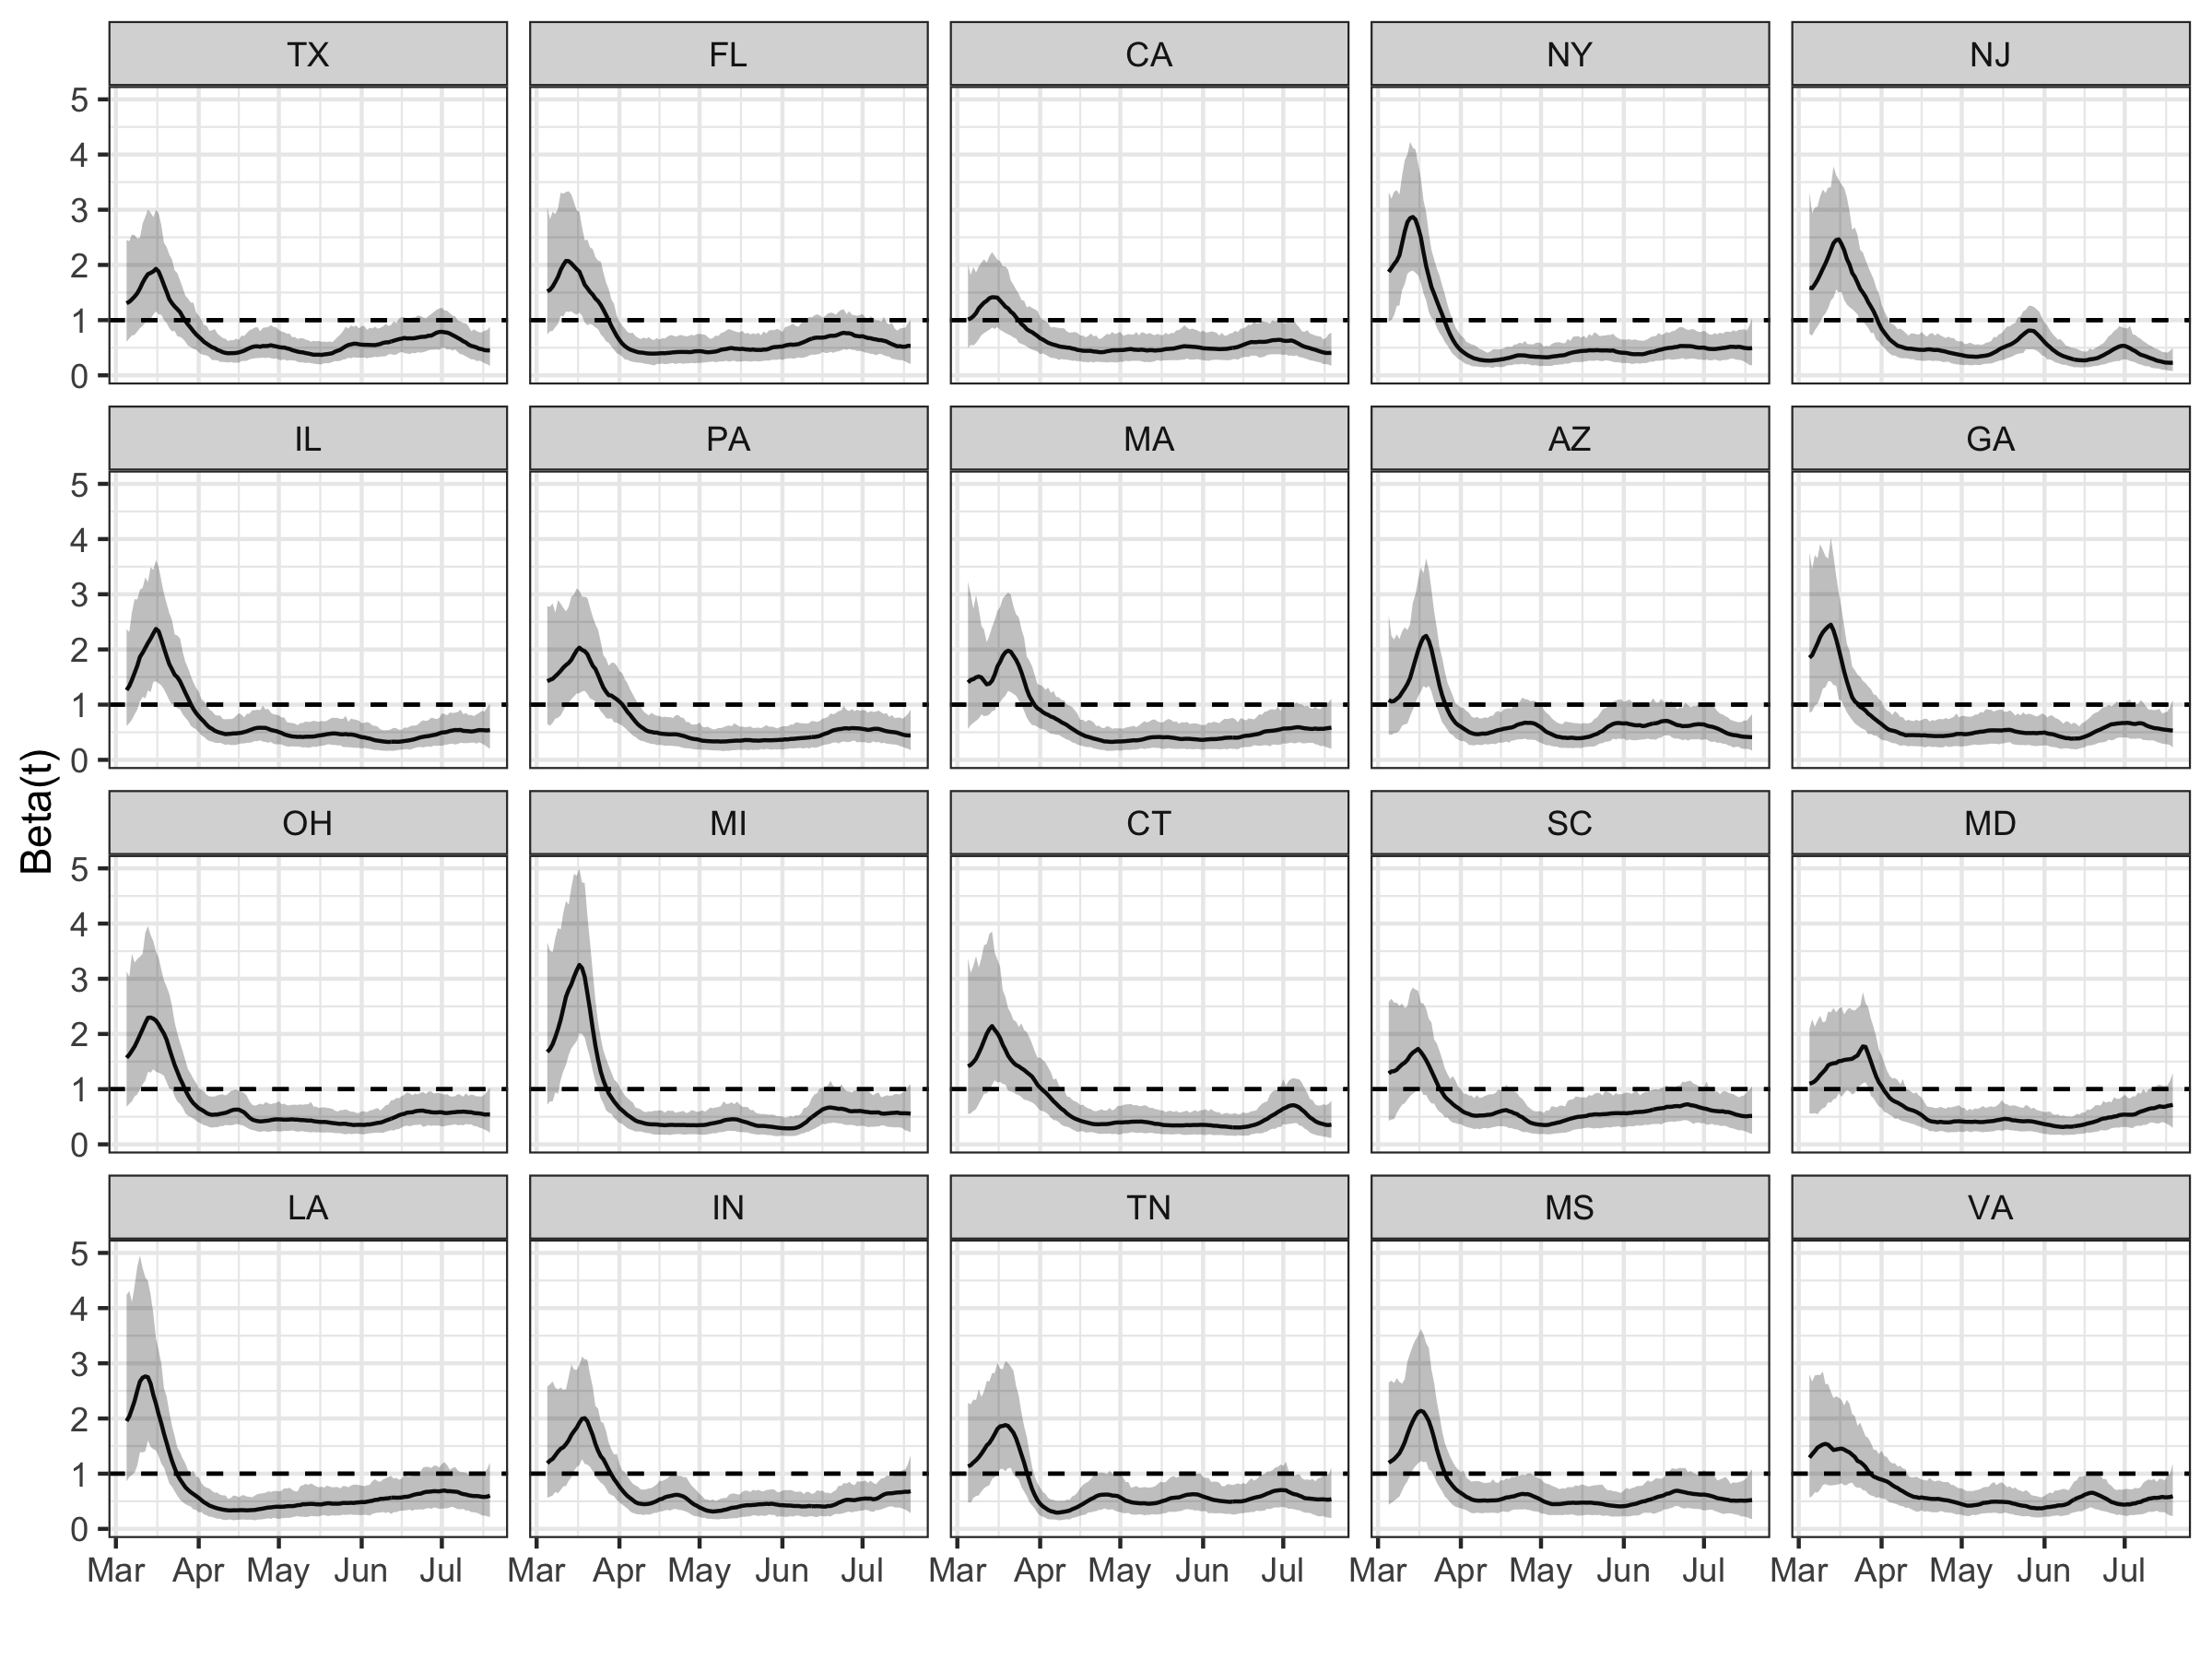
\includegraphics[scale=.15]{beta_t_plot.png}
%    \caption{Time-varying beta ($\beta(t)$).}
%\end{subfigure}
%
%\begin{subfigure}{1\textwidth}
%  \centering
%    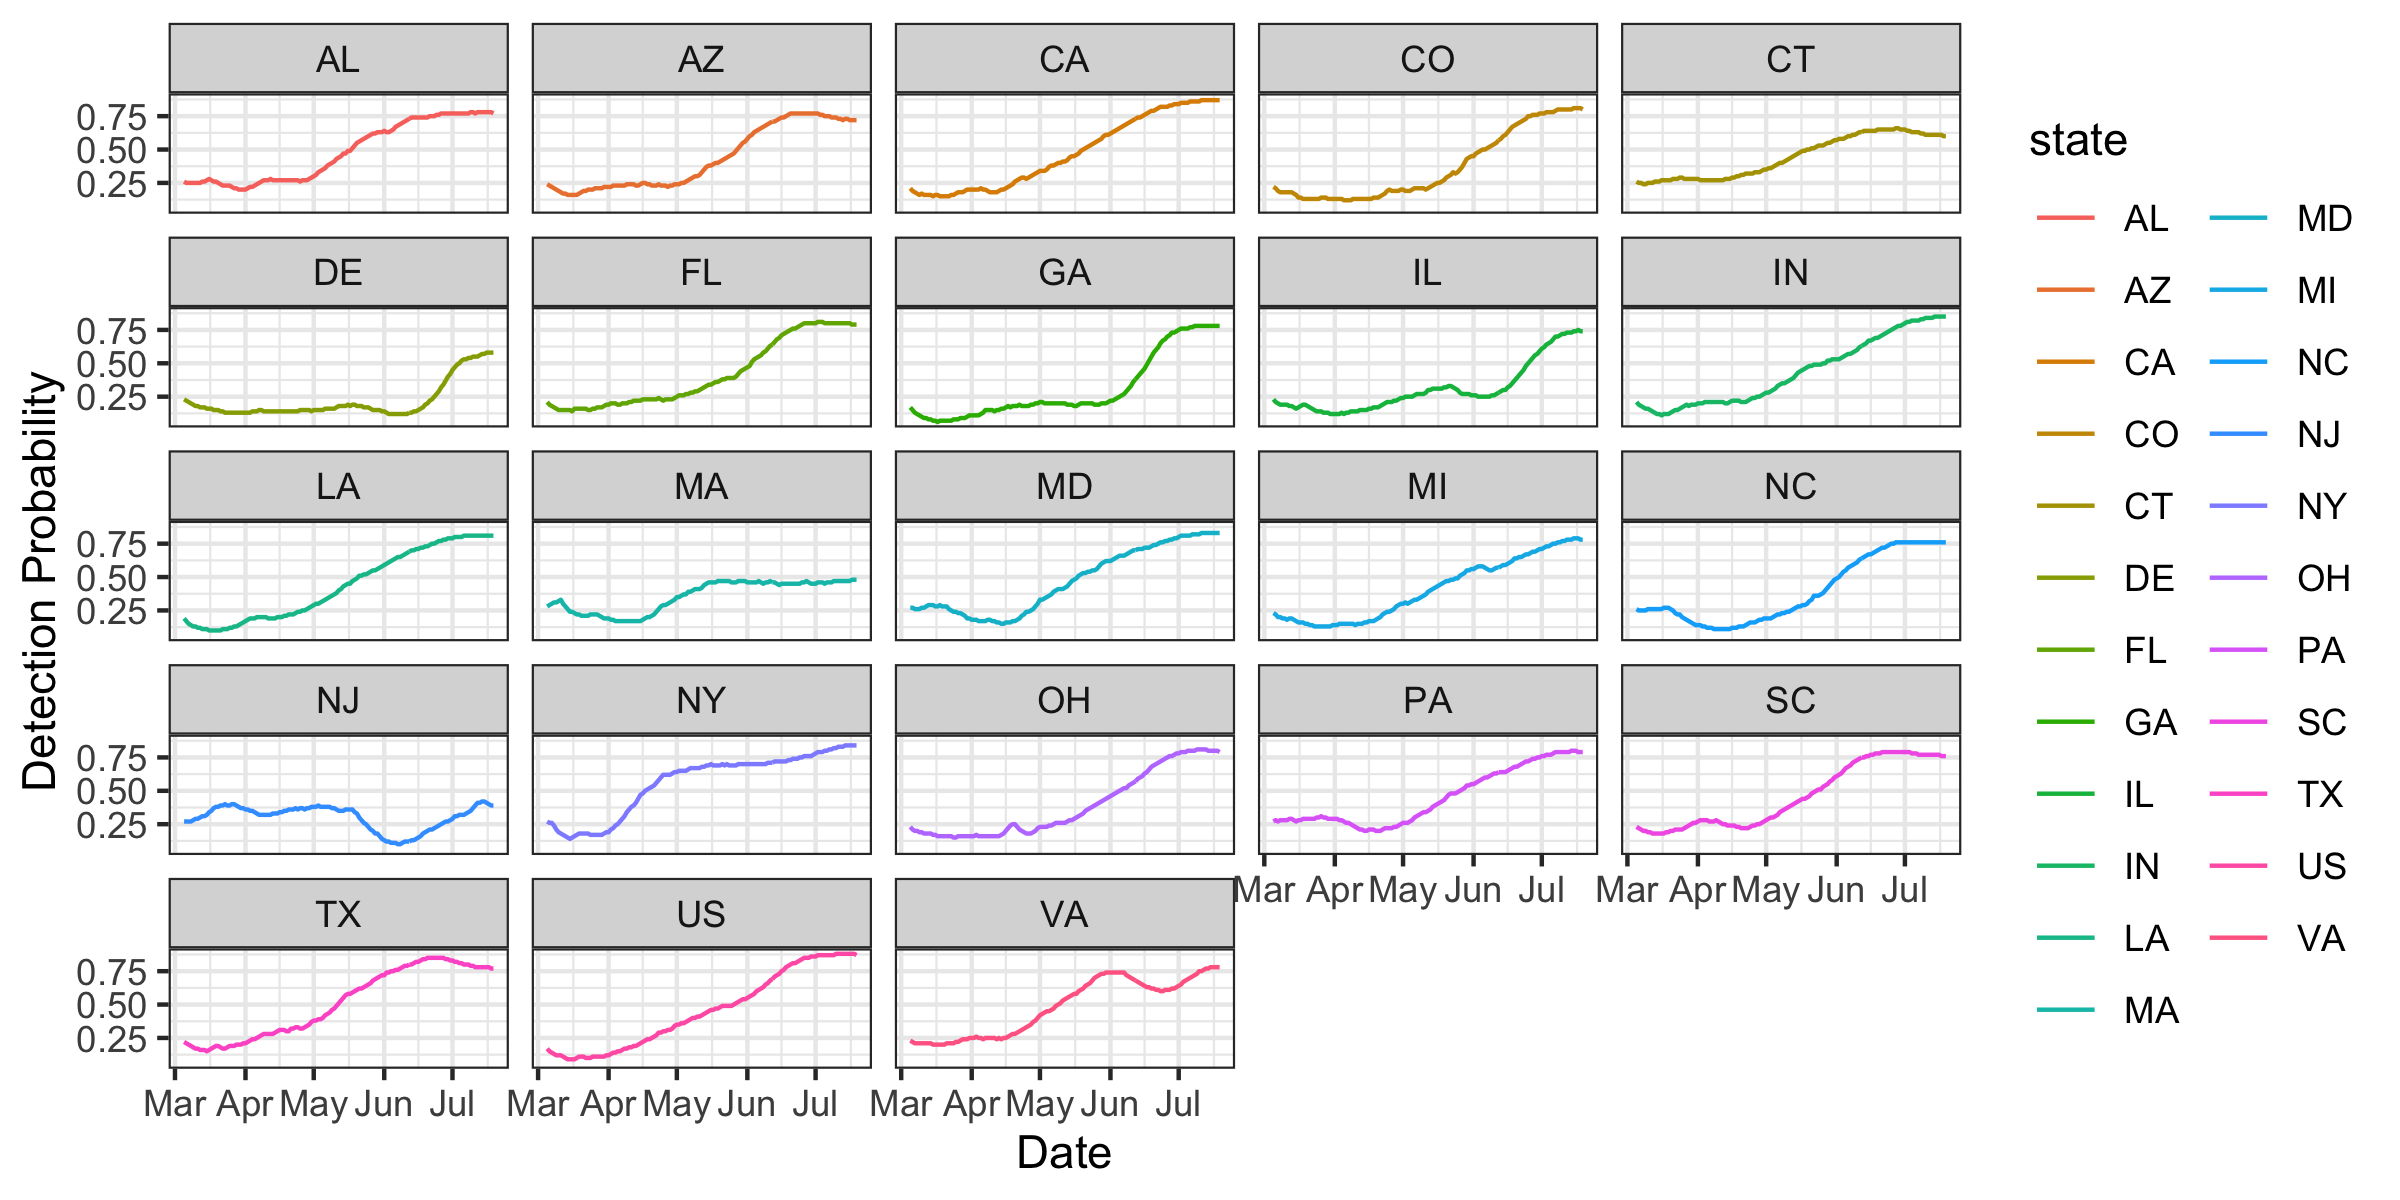
\includegraphics[scale=.15]{detection_plot.png}
%    \caption{Time-varying case and death deviation model ($p_{c,t}$)}
%\end{subfigure} 
% \caption{  A) Time varying beta parameter for all states with a day exceeding 50 incident deaths, including the U.S. by 2020-07-26. We can clearly see that the random walk is able to account for a composite of intervention efforts. B) Time varying case and death deviation model for example states. The time varying case and death deviation model is able account for the increase in testing and other reporting anomolies.}
%\label{fig:model_details}
%\end{figure}
\section{Results}

\subsection{Model Fitting and Inference}

MechBayes is able to accurately model the observed data, adapting to highly variable incident death reporting, variable transmission rates, and overall heterogeneity of incidence curves (Figure \ref{fig:fit_and_forecast_results} A). The model is able to adapt to highly variable incident death reporting, variable transmission rates, and overall heterogeneity of incidence curves. The model is also able capture the uncertainty of the differential equation parameters well enough to produce well calibrated prediction intervals. Figure \ref{fig:fit_and_forecast_results}  shows prediction intervals at the 95\% level, with 92.3\% of observations falling within the bounds for each state. However, we can also see that in some states, such as California and Florida, the model is biased high, with almost all observations outside of the 95\% prediction interval falling below. Figure \ref{fig:fit_and_forecast_results}  also shows 4 weeks of daily forecasts, along with the daily observed incidence for 1 week out. We can see that the predictions are tracking the data even under the highly variable weekly reporting fluctuations. 

MechBayes is able to adapt to changes in transmission through the $\beta(t)$ parameter (Figure \ref{fig:fit_and_forecast_results} C). Transmission was high across all four example states in March, with exponential growth rates shown in panel B. Transmission then slowed significantly in April across each states. While New York remained low through July, Texas, California and Florida saw increases in late June. This is reflected in the increase in incident deaths approximately two weeks later in mid-July.


MechBayes is able to adapt to changes in the case-fatality ratio through the $p_{c,t}$ parameter (Figure \ref{fig:fit_and_forecast_results} D). At the start of the pandemic, only those who were very sick were able to be tested. This lead to an unusually high case-fatality ratio (with respect to estimates from other countries). MechBayes was able to increase the number of latent cases (by a factor of $p_{c,t}$) to lower the estimated case-fatality ratio and avoid extreme over estimates of incident death predictions that would have accompanied such a drastic increase in cases in March. The model was able to adapt to this change across all four example states. 




%Note that interpreting this strictly as time-varying detection is obscuring the fact that this parameter $p_{t,d}$ can soak-up any excess variation beyond the ability of cases and the case-fatility ratio to explain the number of deaths. That is, the time-varying case and death deviation model is able to "de-couple" cases and deaths beyond the case-fataility ratio regardless of the underlying reason (whether that be an increase in testing or shifting age distribution of cases). Thus, interpretation of this parameter as a strict mapping to testing is incorrect. As a forecasting model, we only need the ability to non-parametrically model deviations and reporting issues in cases.



\begin{figure}
  \centering
     \begin{subfigure}{.5\textwidth}
  \centering
    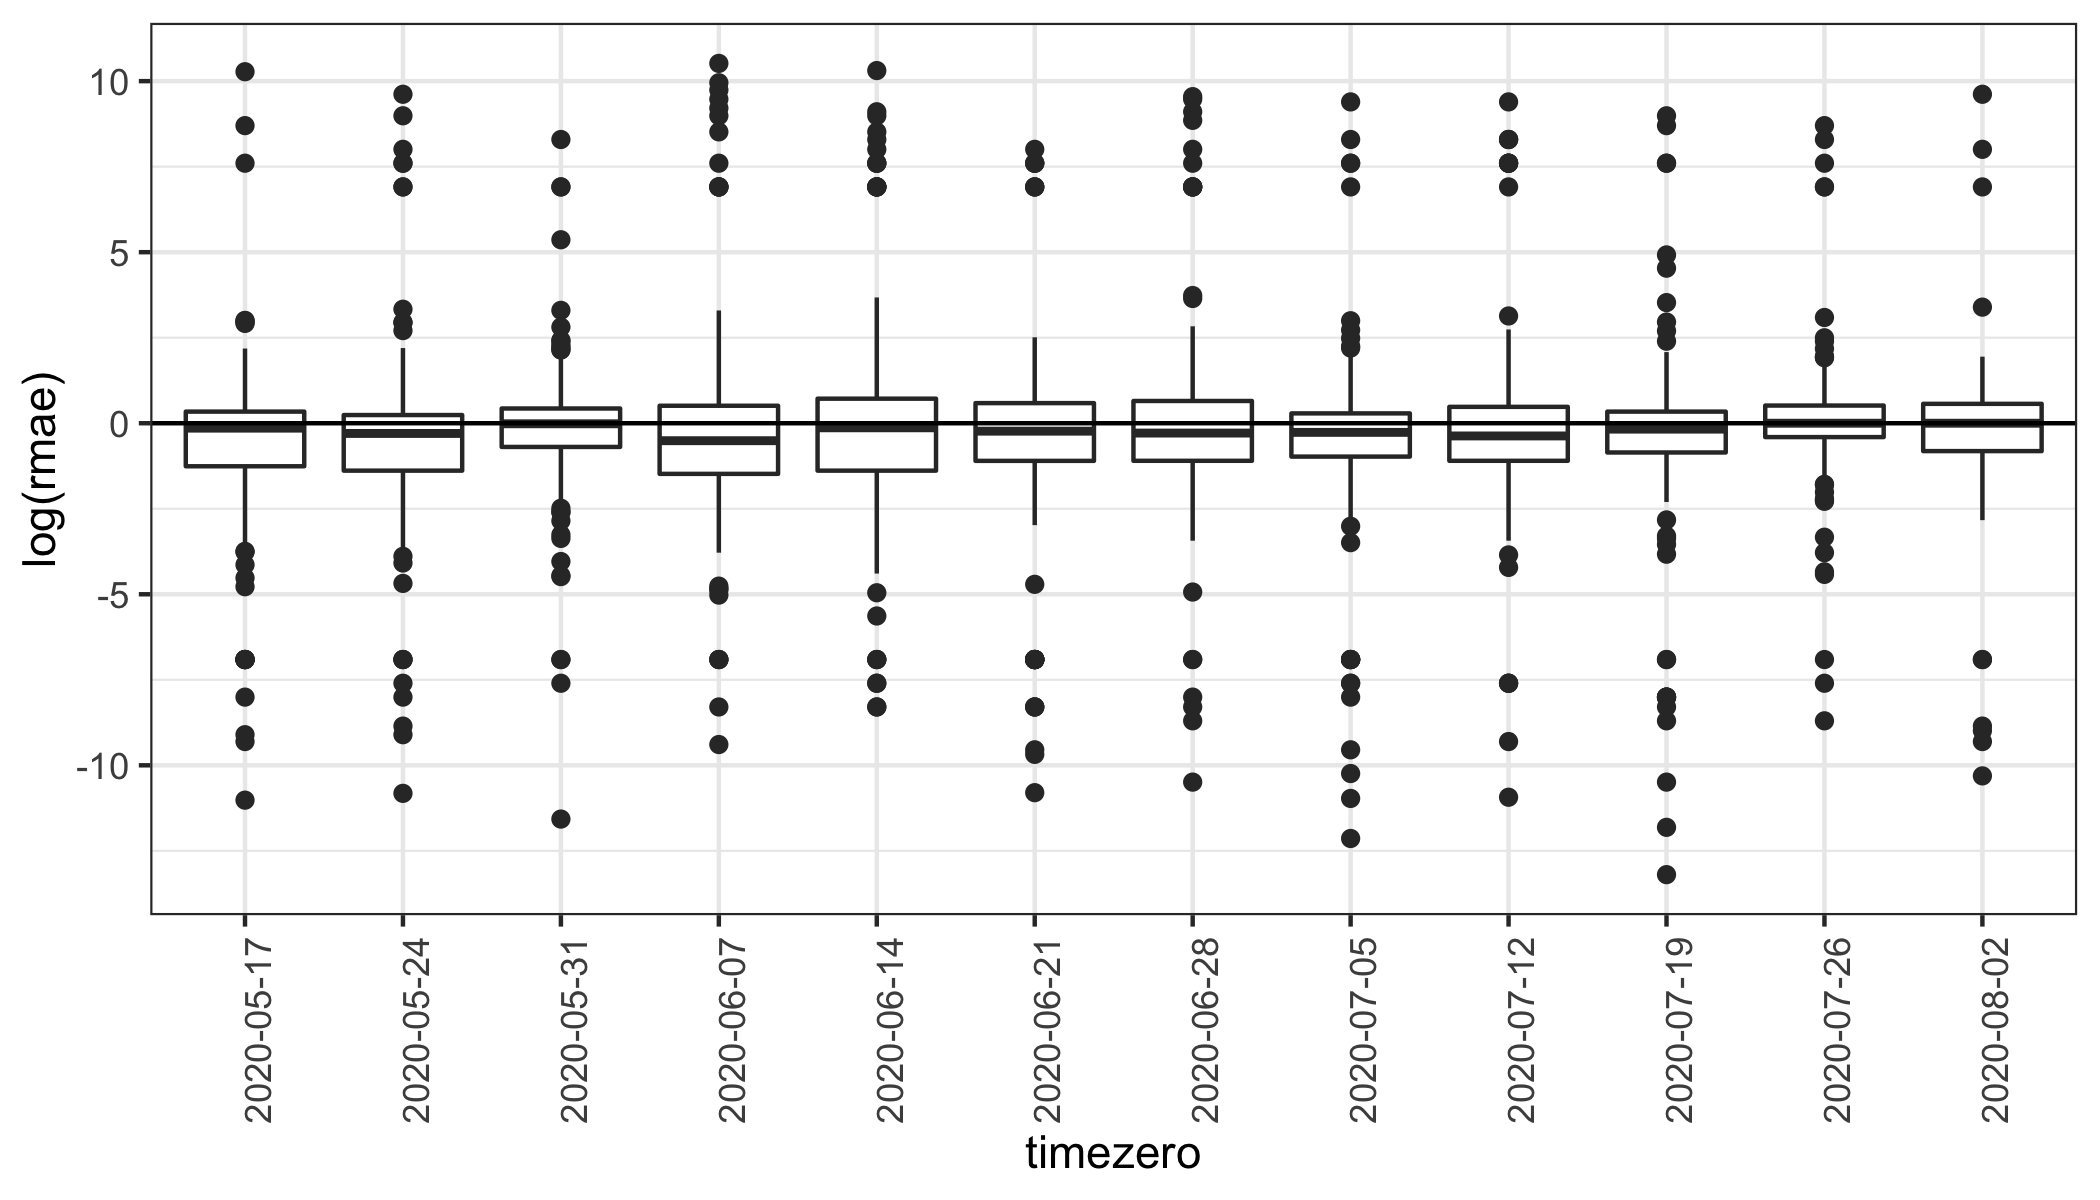
\includegraphics[scale=.135]{mae_results_by_time_zero_inc.png}
    \caption{MAE by forecast week}
\end{subfigure}%
\begin{subfigure}{.5\textwidth}
  \centering
    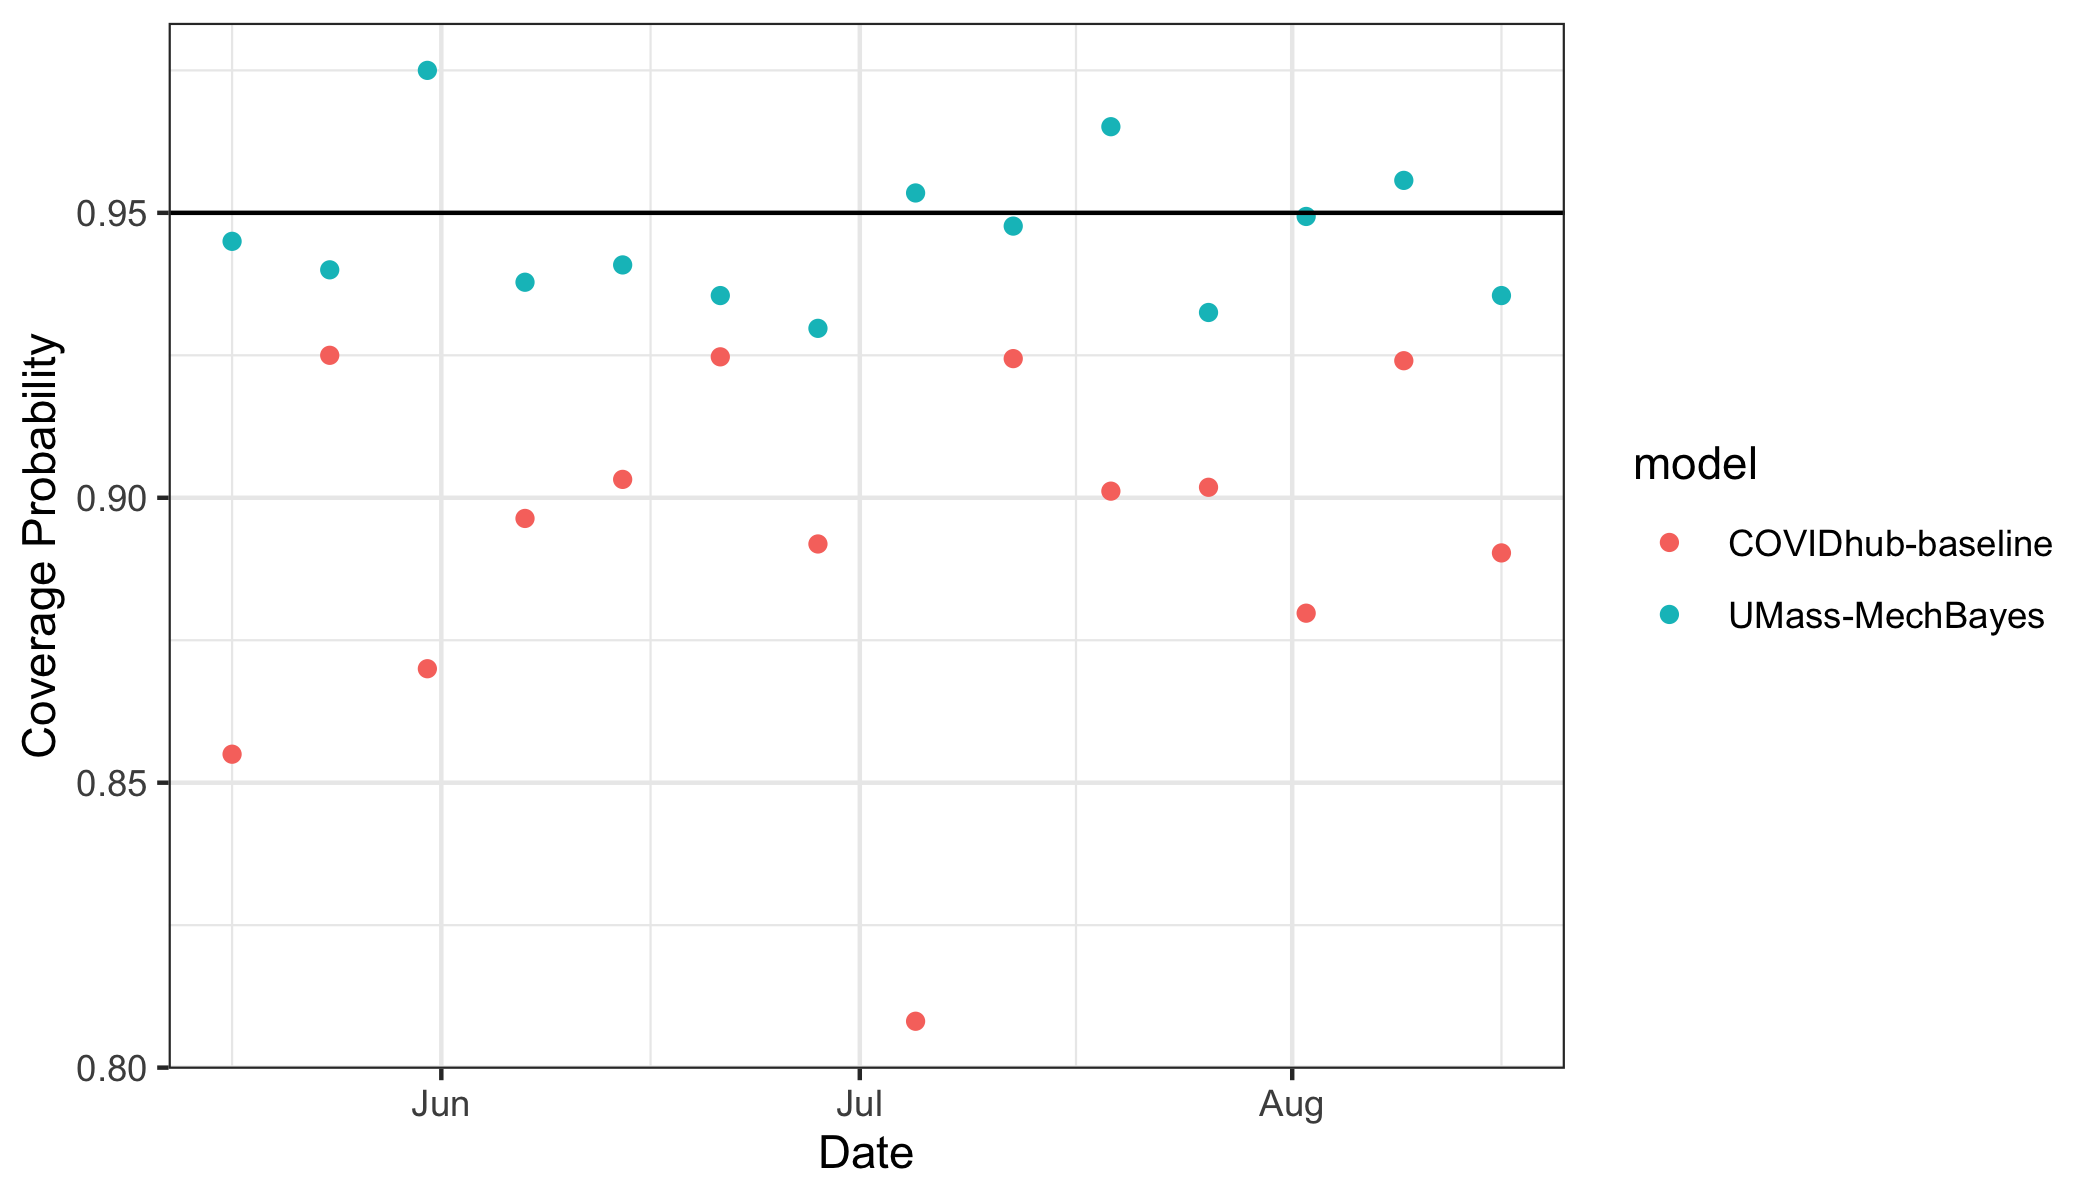
\includegraphics[scale=.115]{cp_results_by_time_zero.png}
    \caption{Coverage probability by forecast week}
\end{subfigure}
\begin{subfigure}{.5\textwidth}
  \centering
    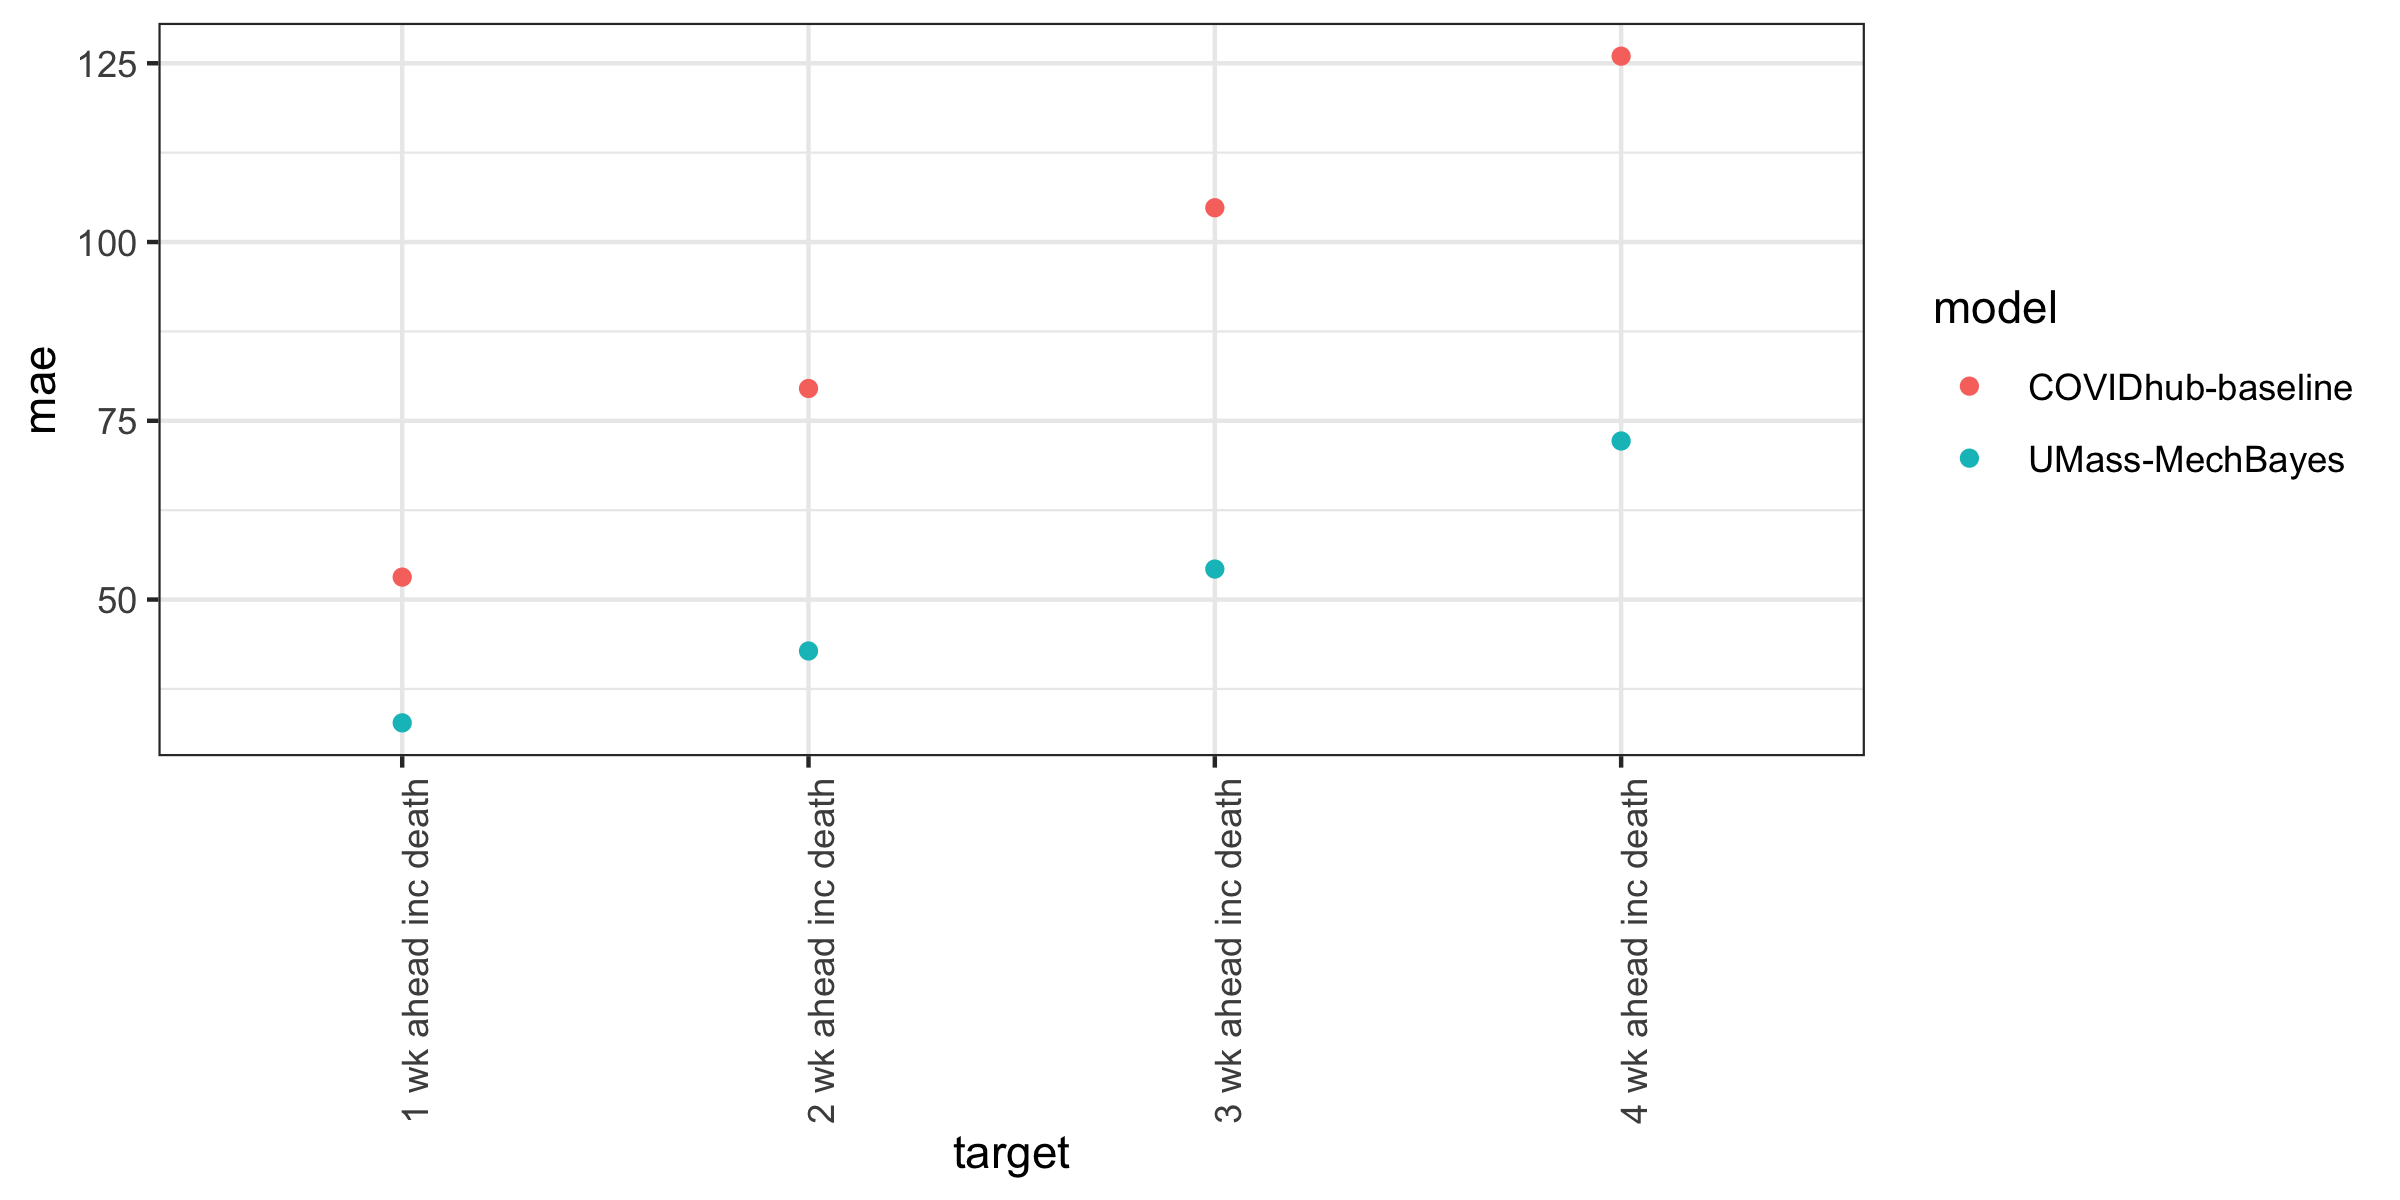
\includegraphics[scale=.135]{mae_results_by_target_inc.png}
    \caption{MAE by target}
\end{subfigure}%
\begin{subfigure}{.5\textwidth}
  \centering
    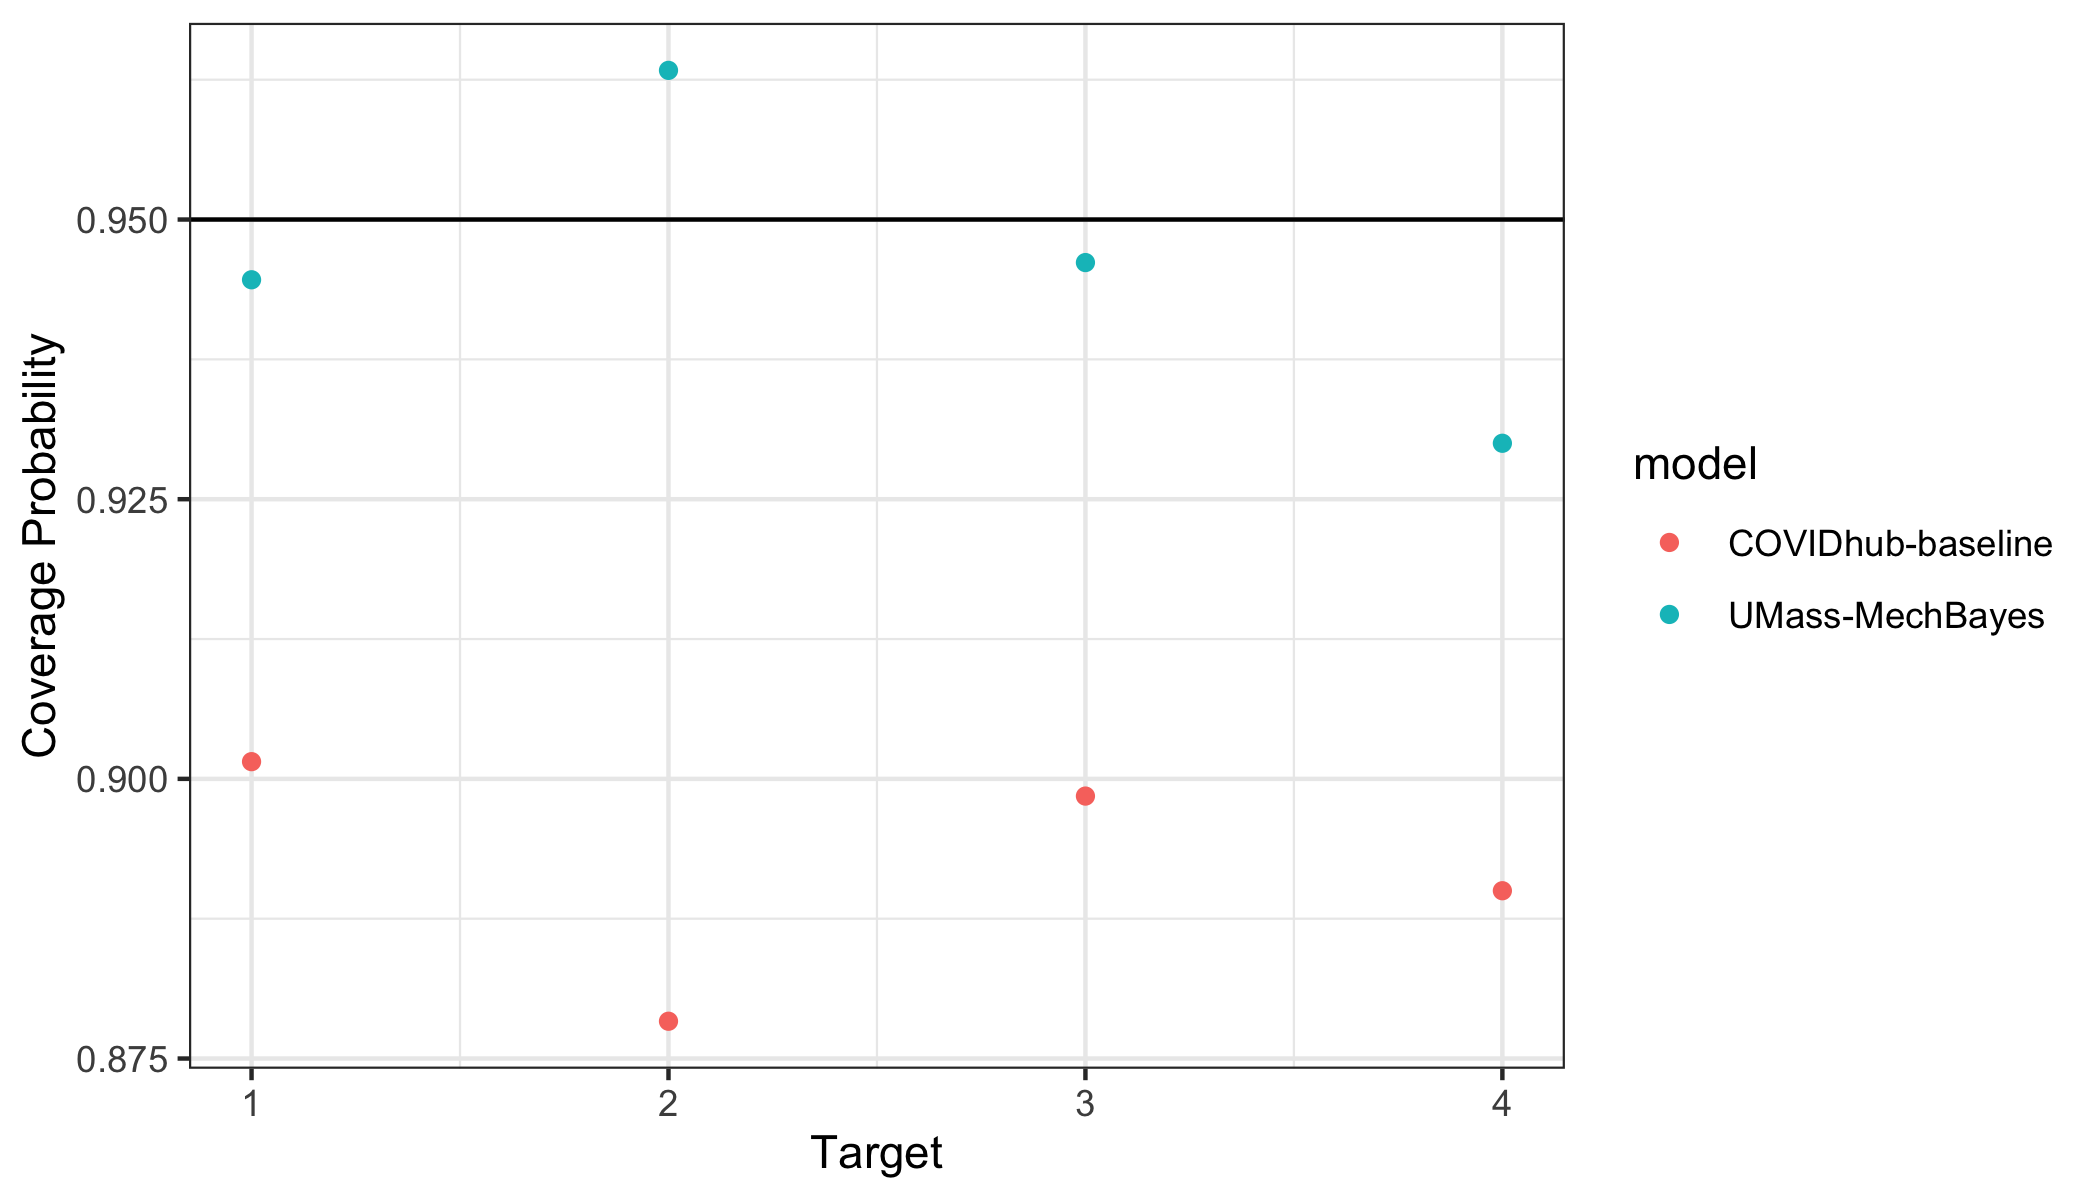
\includegraphics[scale=.115]{cp_results_by_target.png}
    \caption{Coverage probability by target}
\end{subfigure}%

\caption{Scores from CDC COVID-19 forecast initiative broken down by target and forecast week. In Panels A and B, each observation represents mean absolute error (MAE) and empirical prediction interval coverage rate averaged across all targets and locations for the given week in which forecasts were made. MechBayes improves in average MAE in 9 out of 12 timepoints. MechBayes improves in MAE across all targets. We can see that as the horizon increases from 1 to 4 weeks ahead, MAE, reflecting an increase in difficulty of forecasting further ahead in time. We also see a uniform improvement in coverage probability when broken down by timezero and target. Here the horizontal line represents 95\% coverage interval. }
\label{fig:covidhub}
\end{figure}


\begin{figure}
  \centering

\begin{subfigure}{\textwidth}
  \centering
    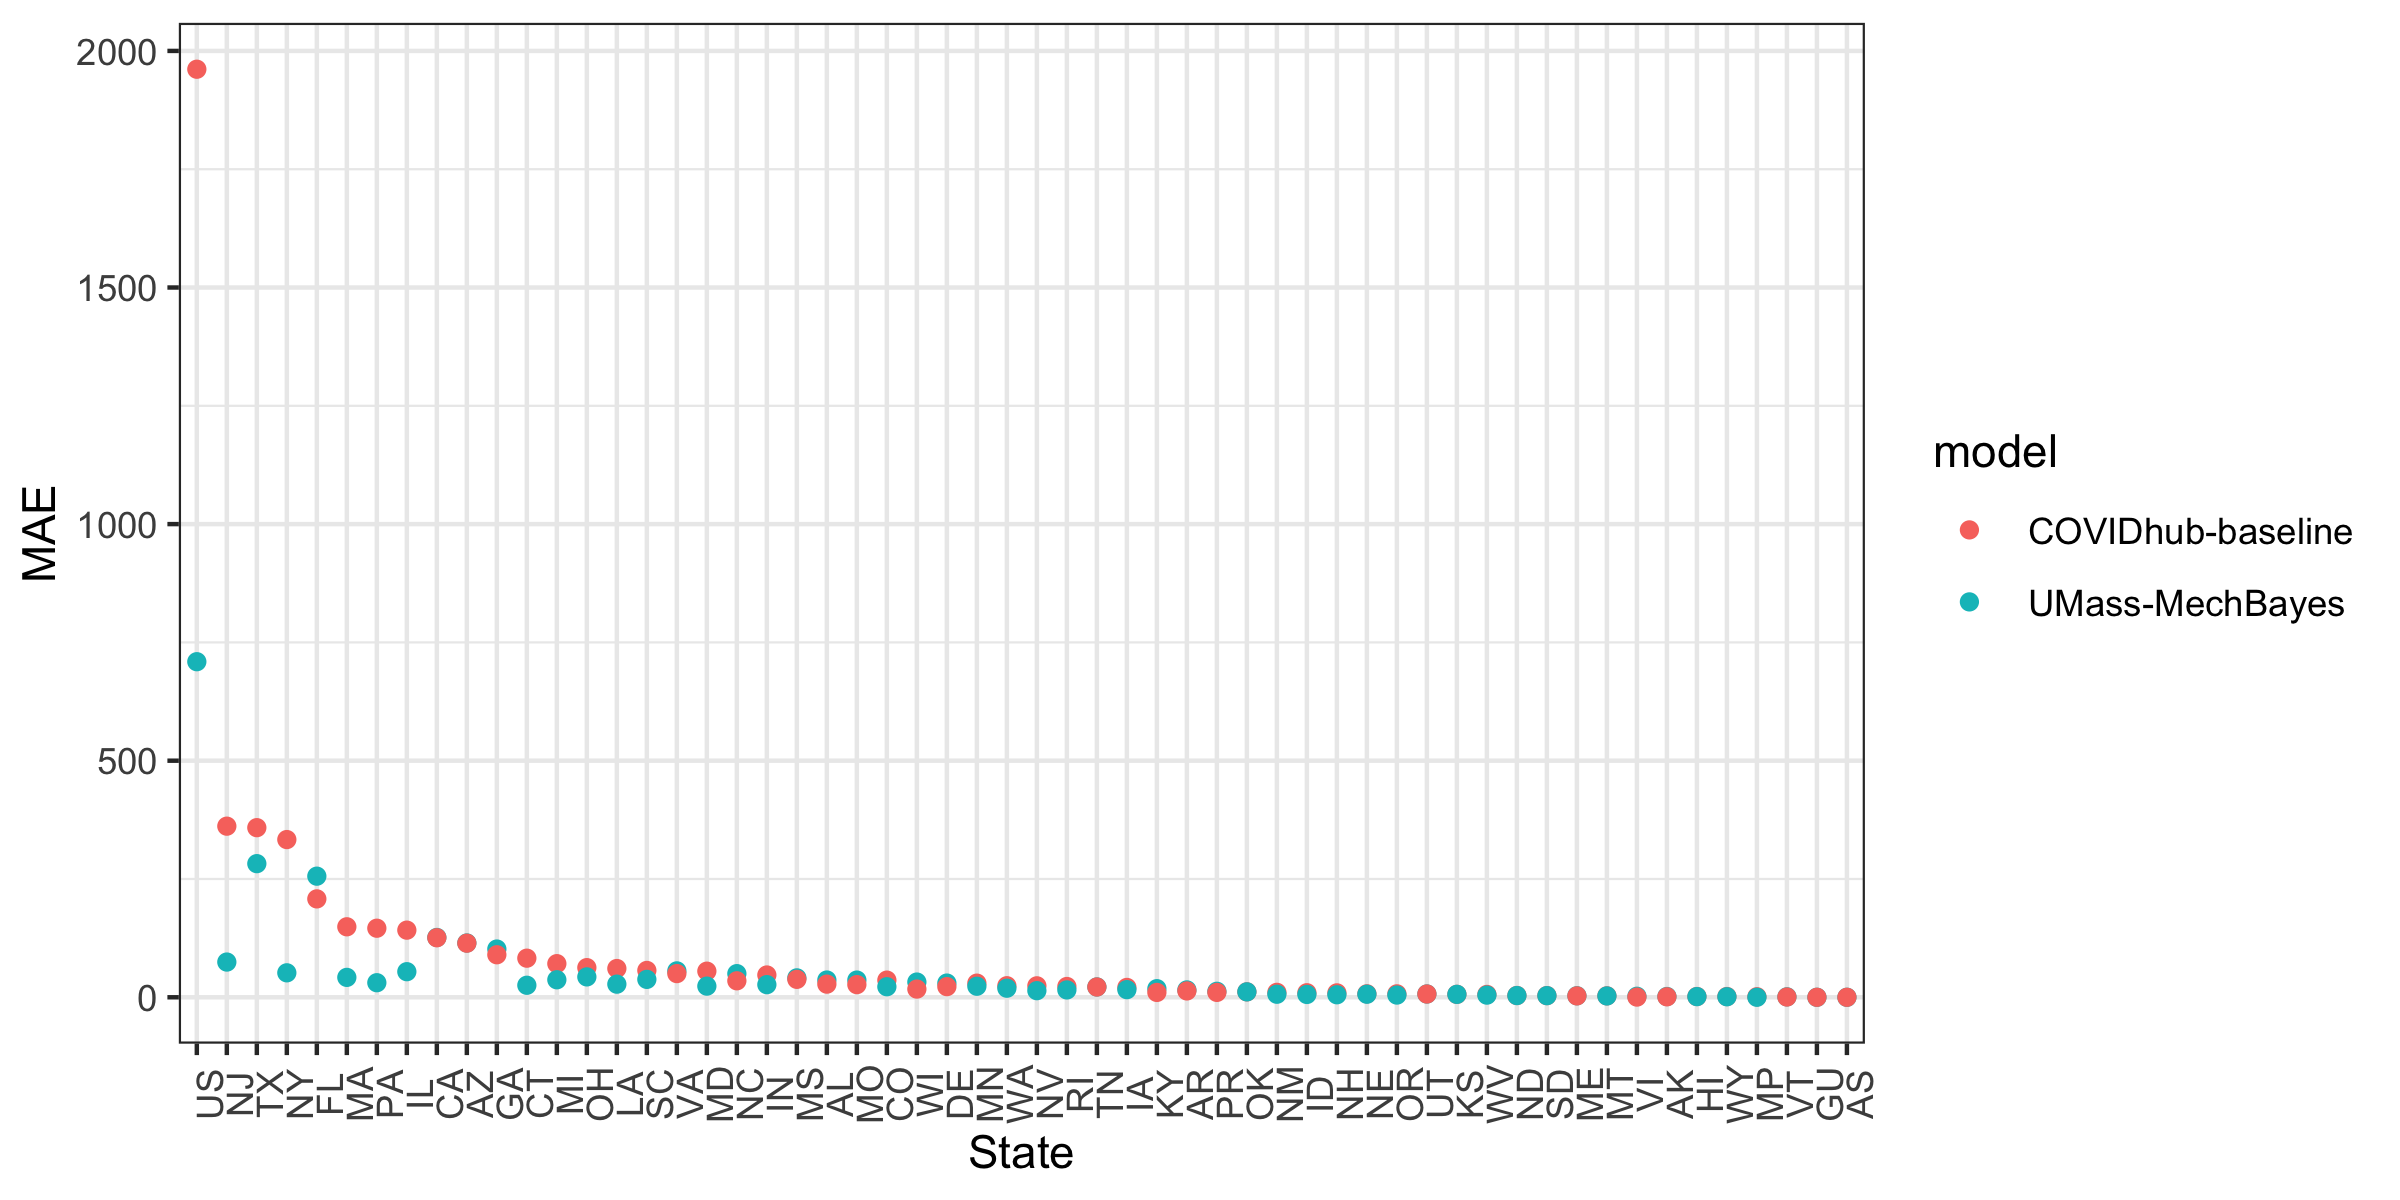
\includegraphics[scale=.2]{mae_results_by_region_inc.png}
    \caption{MAE by region}
\end{subfigure}
\begin{subfigure}{\textwidth}
  \centering
    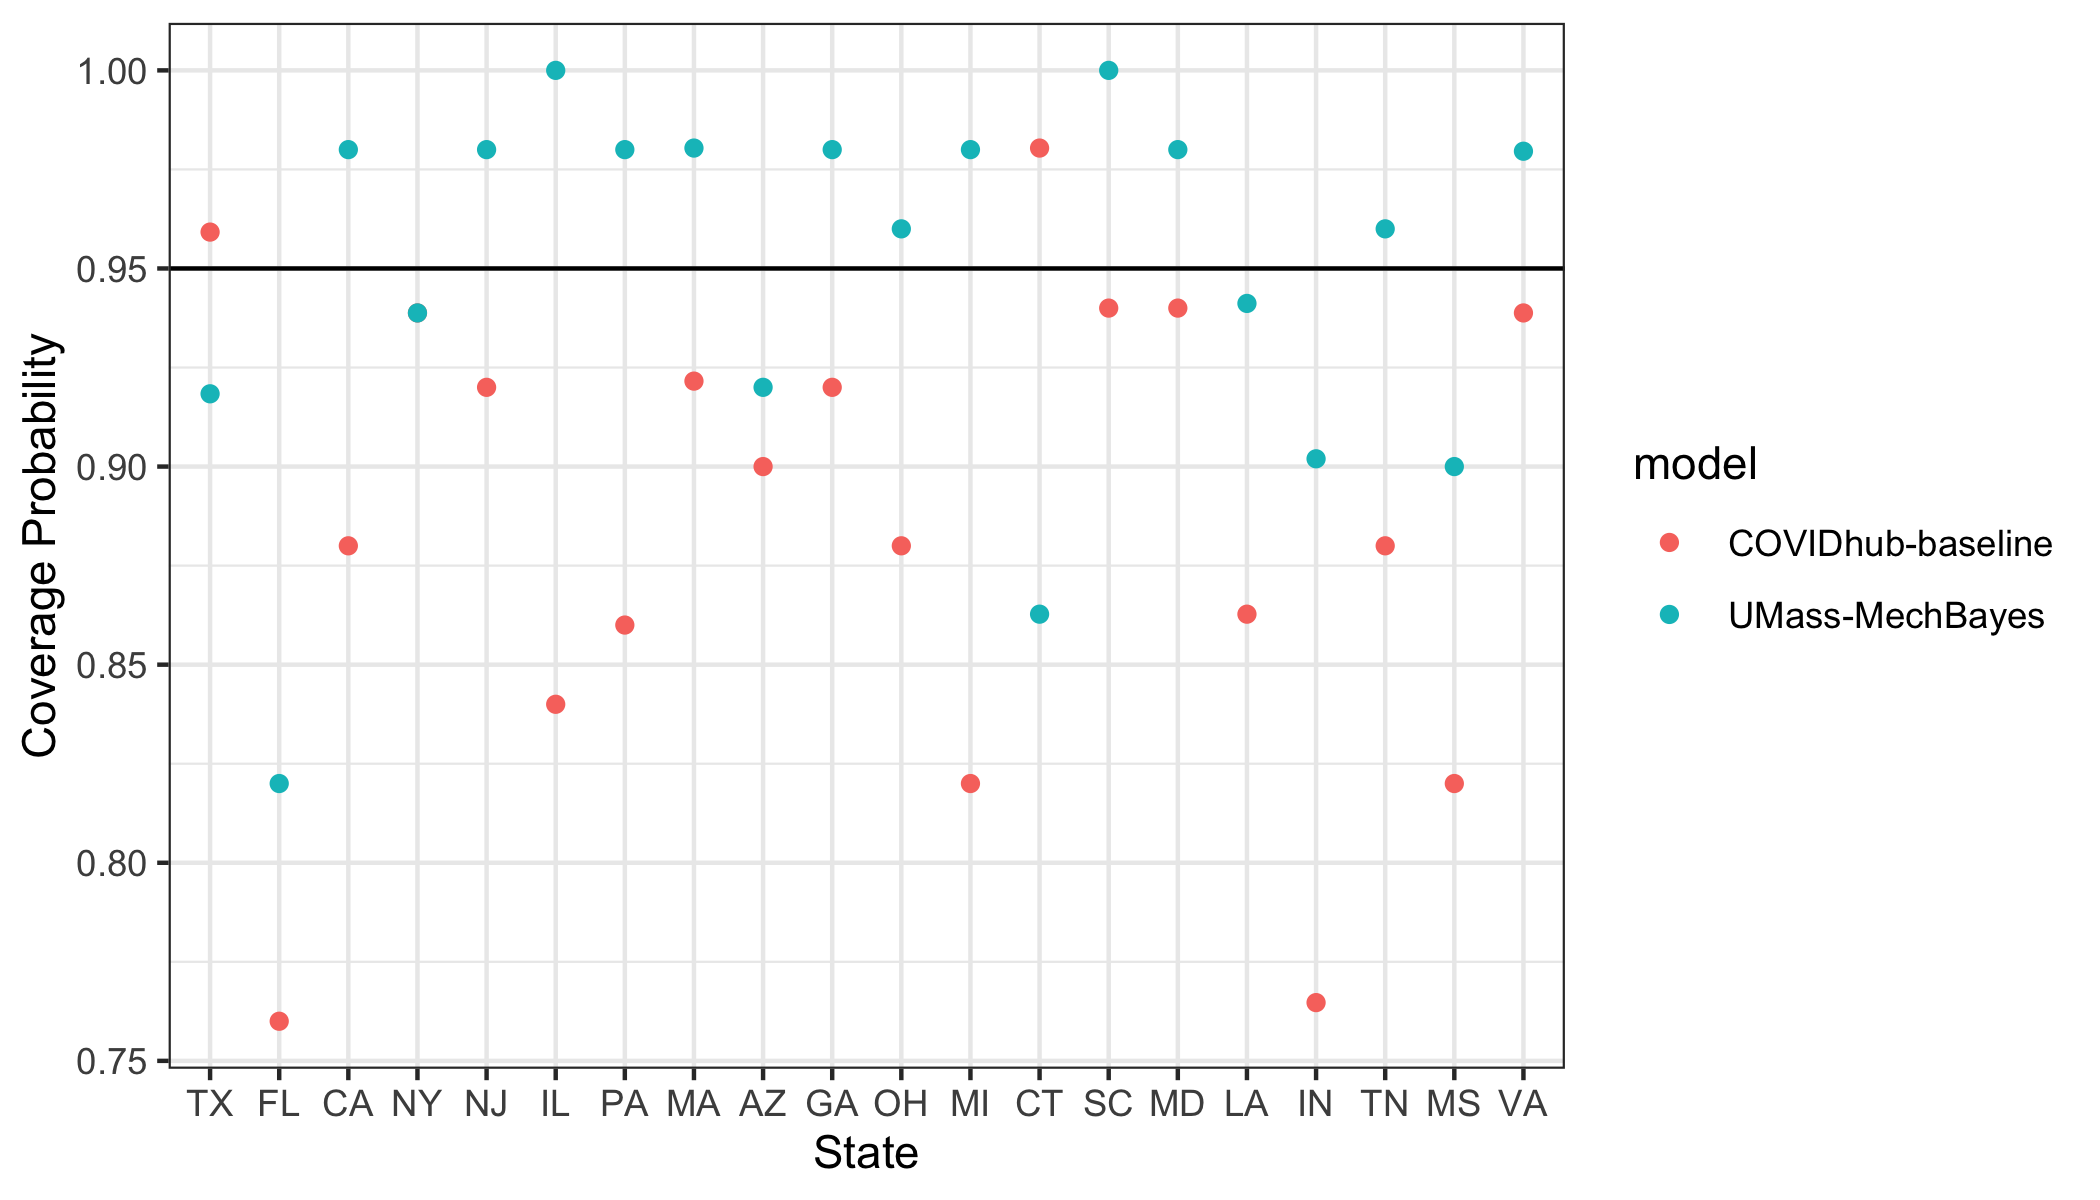
\includegraphics[scale=.20]{cp_results_by_location.png}
    \caption{Coverage probability by region}
\end{subfigure}
\caption{Scores from CDC COVID-19 forecast initiative broken down by region for the 20 regions with the highest incident deaths. Each observation represents mean absolute error (MAE) or empirical prediction interval coverage rate averaged across all targets and forecast dates for the given region in which forecasts were made. Regions are sorted by total deaths left to right. Here we can see that MechBayes has the greatest increase in states with large total death counts. States with medium or small death counts have more mixed results. The improvements in coverage probability are more mixed, with MechBayes improving coverage probability in 12 of 20 regions. }
\label{fig:covidhub_region_results}
\end{figure}


\subsection{CDC Forecast Results}

We next turn to the comparison of MechBayes against the CDC baseline model. This baseline model uses the previous daily incident as the mean forecast for the current daily incidence, along with  bootstrapped prediction intervals from historical changes in daily incidence. See CDC COVID-19 Forecast Hub for more details \cite{covidhub}. 

Overall, MechBayes had an MAE of 34.1, when averaging over all regions, forecast dates, and targets. The CDC baseline model had an MAE of 53.2. Similarly, the empirical coverage probability at the 95\% level for MechBayes was 94.6\%, compared to 93.2\% for the baseline model.

 We also break down the results by week the forecast was made (forecast week) and averaging over both region and target. As we can see from Figure \ref{fig:covidhub} (A,B), MechBayes outperformed the CDC baseline on MAE and coverage probability when broken down by forecast week. While the improvements broken down by time are small, there is an improvment in 9 out of 12 evaluation weeks in MAE.  As we can see from \ref{fig:data}, in weeks with the largest increase in deaths (mostly during the month of May) MechBayes significantly outperformed the baseline model. However, in weeks with a small increase or a decrease in deaths, the scores were much closer. This suggests that MechBayes performs well where it counts, when the epidemic is taking off nearly exponentially. 

We also break down the results by geographical region, as seen in Figure \ref{fig:covidhub} (C,D). Here we see consistent improvements in MAE under MechBayes for regions with high total death counts with an improvement in the average MAE in 16 out of the 20 states with the highest total death count. Out of the states with the 10 highest death counts, only in California did the baseline model outperform MechBayes on the average MAE. 
We break down the results by target by averaging over region and forecast week  \ref{fig:covidhub} (E,F) Here we can see uniform improvement over the baseline model by MechBayes in terms of MAE and coverage probability. We can also see that the MAE increase as horizon increase, which is to be expected. We can also see that incident MAE is lower than cumulative MAE, which is again to be expected due to the lower absolute numbers of incident deaths. 

Finally, we include a formal test of the difference in MAE to demonstrate statistically significant advantages in using MechBayes over the baseline model. MechBayes has statistically significantly lower MAE for 1-4 weeks ahead at the 95\% level (coefficients in Appendix 2). The difference in skill seems to improve as the forecast horizon increases. For example, if the baseline model MAE for a particular 1 step ahead forecast is 30, one would expect the MechBayes forecast to have an MAE of 24.8.  If the baseline model MAE for a particular 4 step ahead forecast is 30, one would expect the MechBayes forecast to have an MAE of 22.5.  We demonstrate that the mixed model proposed above fits the MAE results reasonably in Appendix 2.


 \subsection{Ablation Test Results}

MechBayes Case/Death Time-Varying is consistently better than MechBayes Death Fixed or MechBayes Case/Death Fixed. The only exception seems to be June 22nd 2020 for the two week ahead target. The difference in MAE between MechBayes Case/Death Time-Varying and the competing models increases as forecast horizon increases. This suggest that MechBayes Case/Death Time-Varying is a better long term forecasting model.

We can also see that the MechBayes Death Fixed is consistently better than MechBayes Case/Death Fixed.  This may be evidence that naively including case data, without adjusting for discrepancies between cases and deaths due to testing etc., may be worse than not including it at all. 

\begin{figure}
  \centering
     \begin{subfigure}{.5\textwidth}
  \centering
    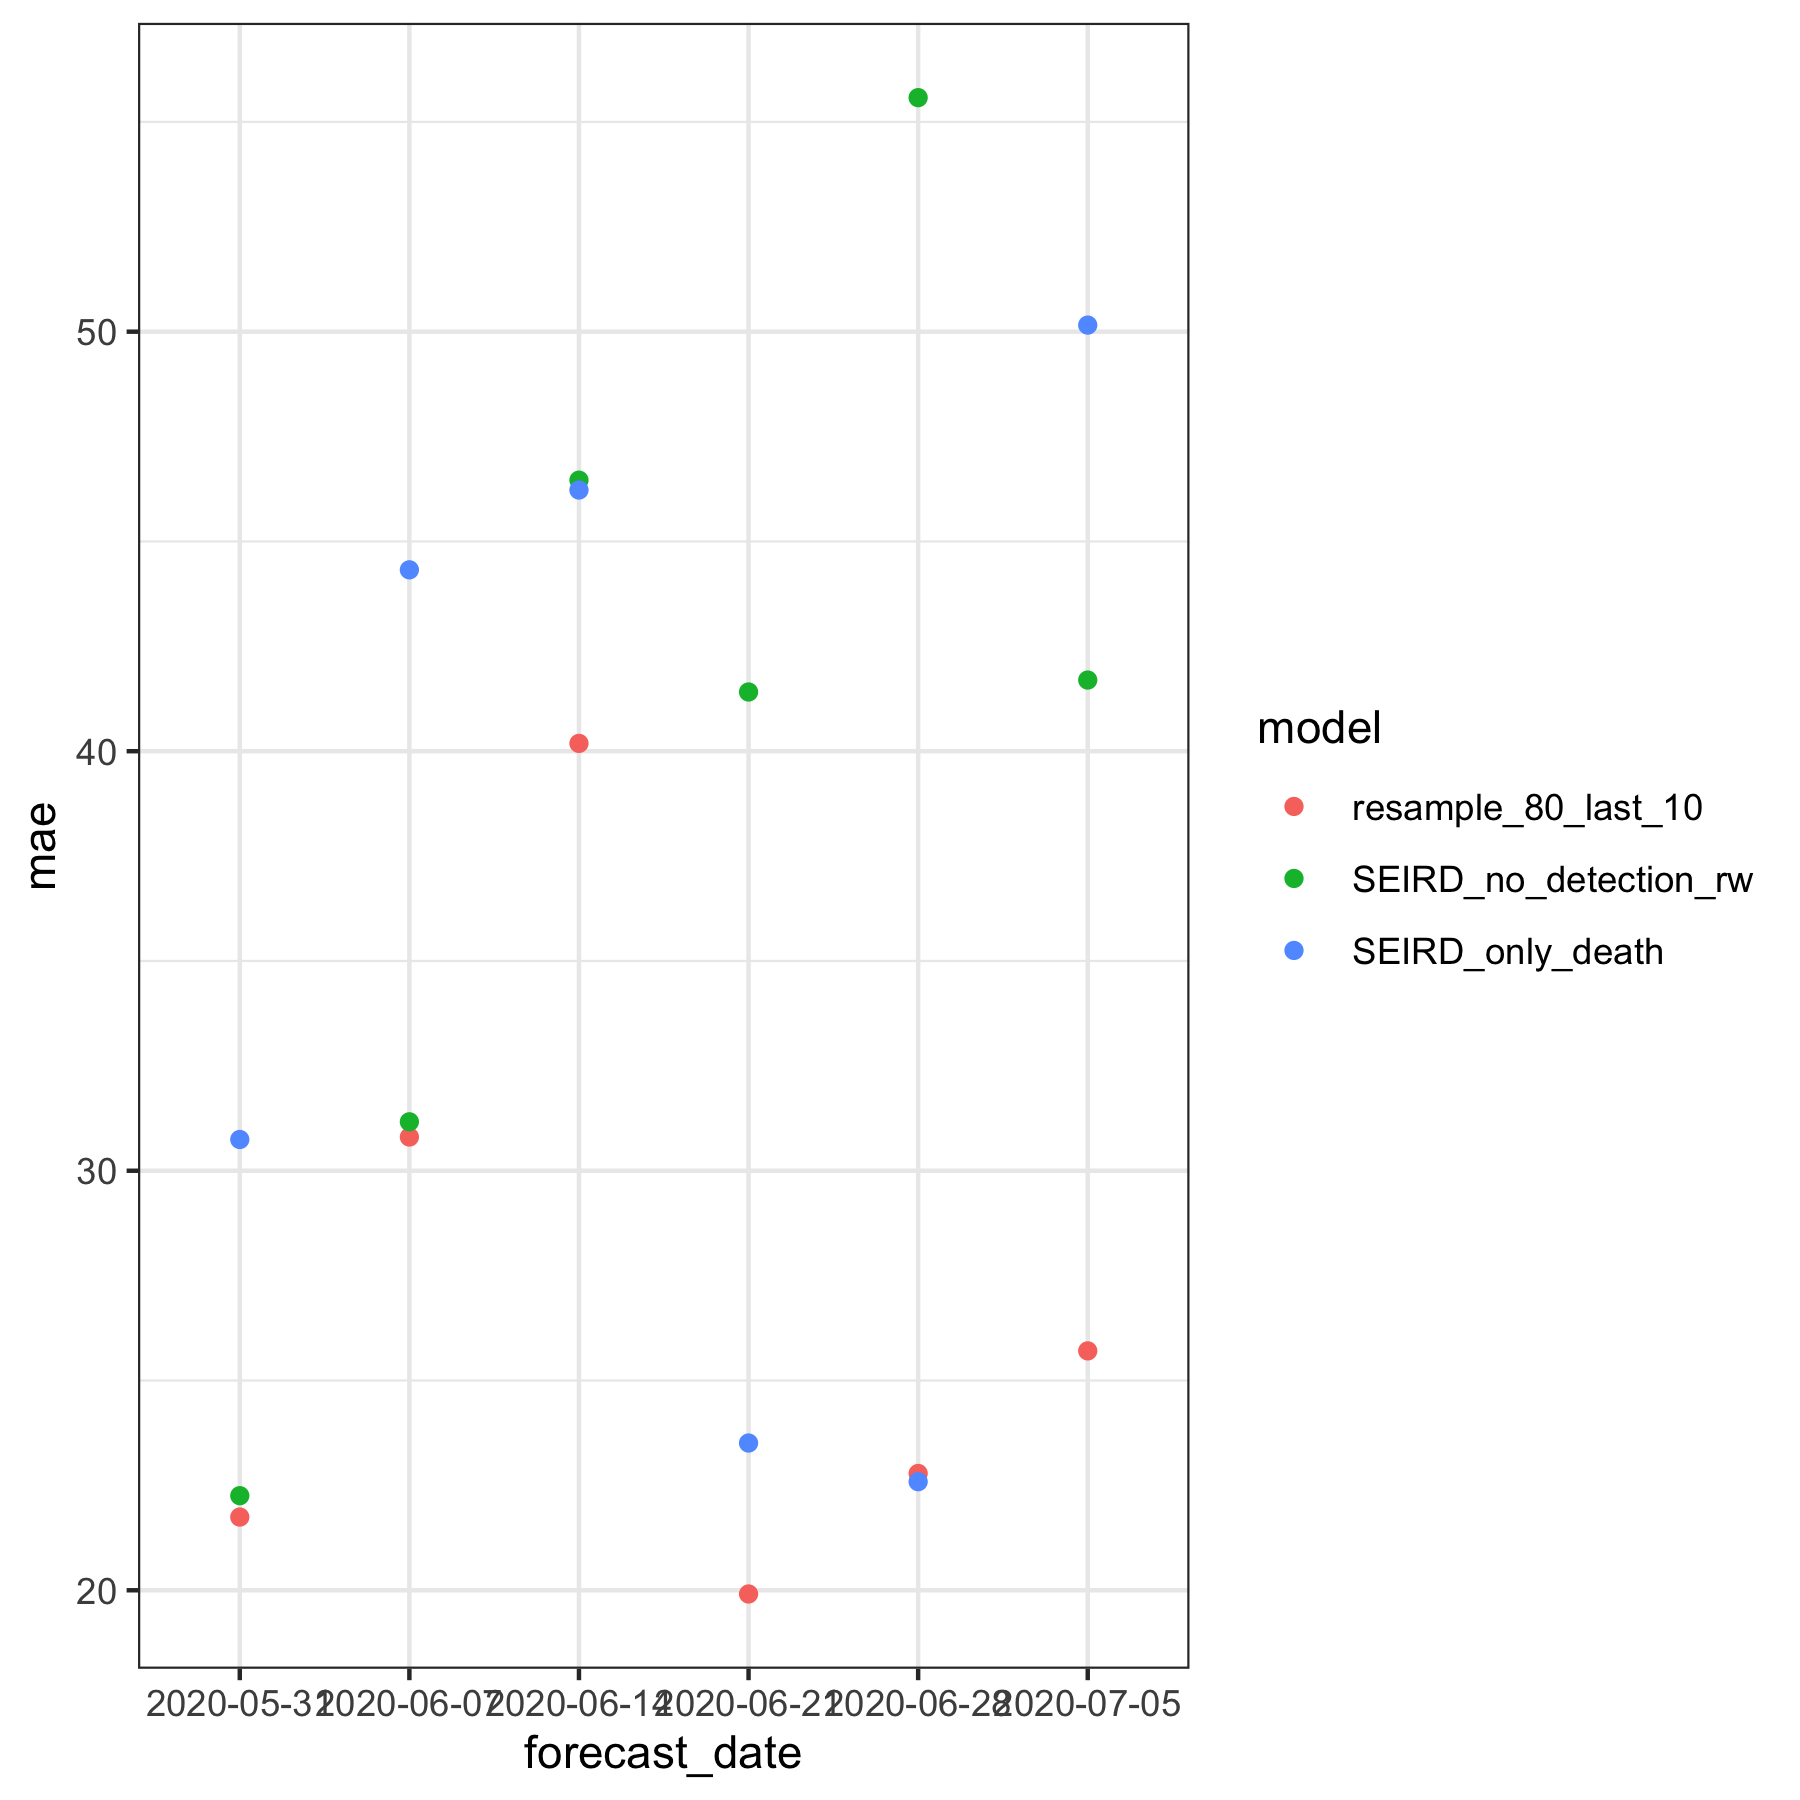
\includegraphics[scale=.15]{ablation_1.png}
    \caption{1 week ahead.}
\end{subfigure}%
\begin{subfigure}{.5\textwidth}
  \centering
    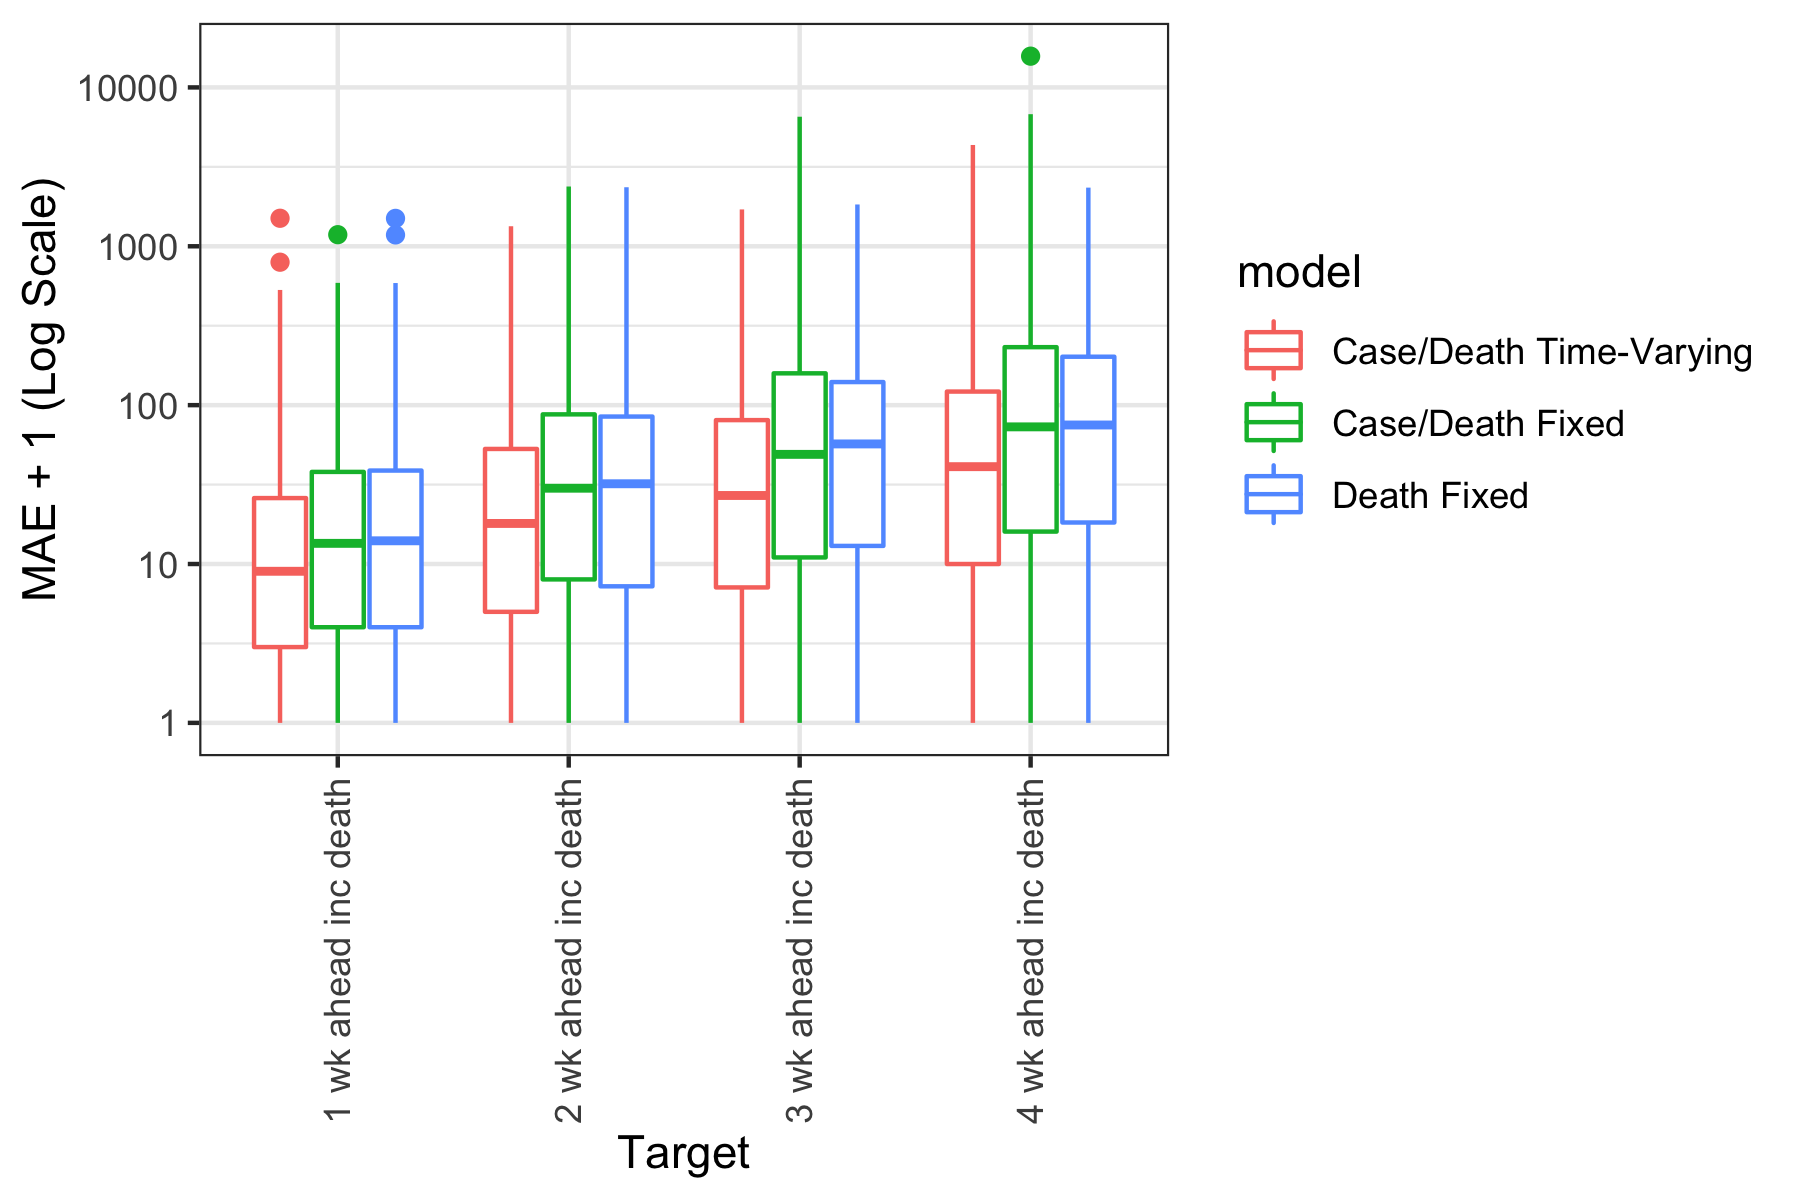
\includegraphics[scale=.15]{ablation_2.png}
    \caption{2 week ahead.}
\end{subfigure}
\begin{subfigure}{.5\textwidth}
  \centering
    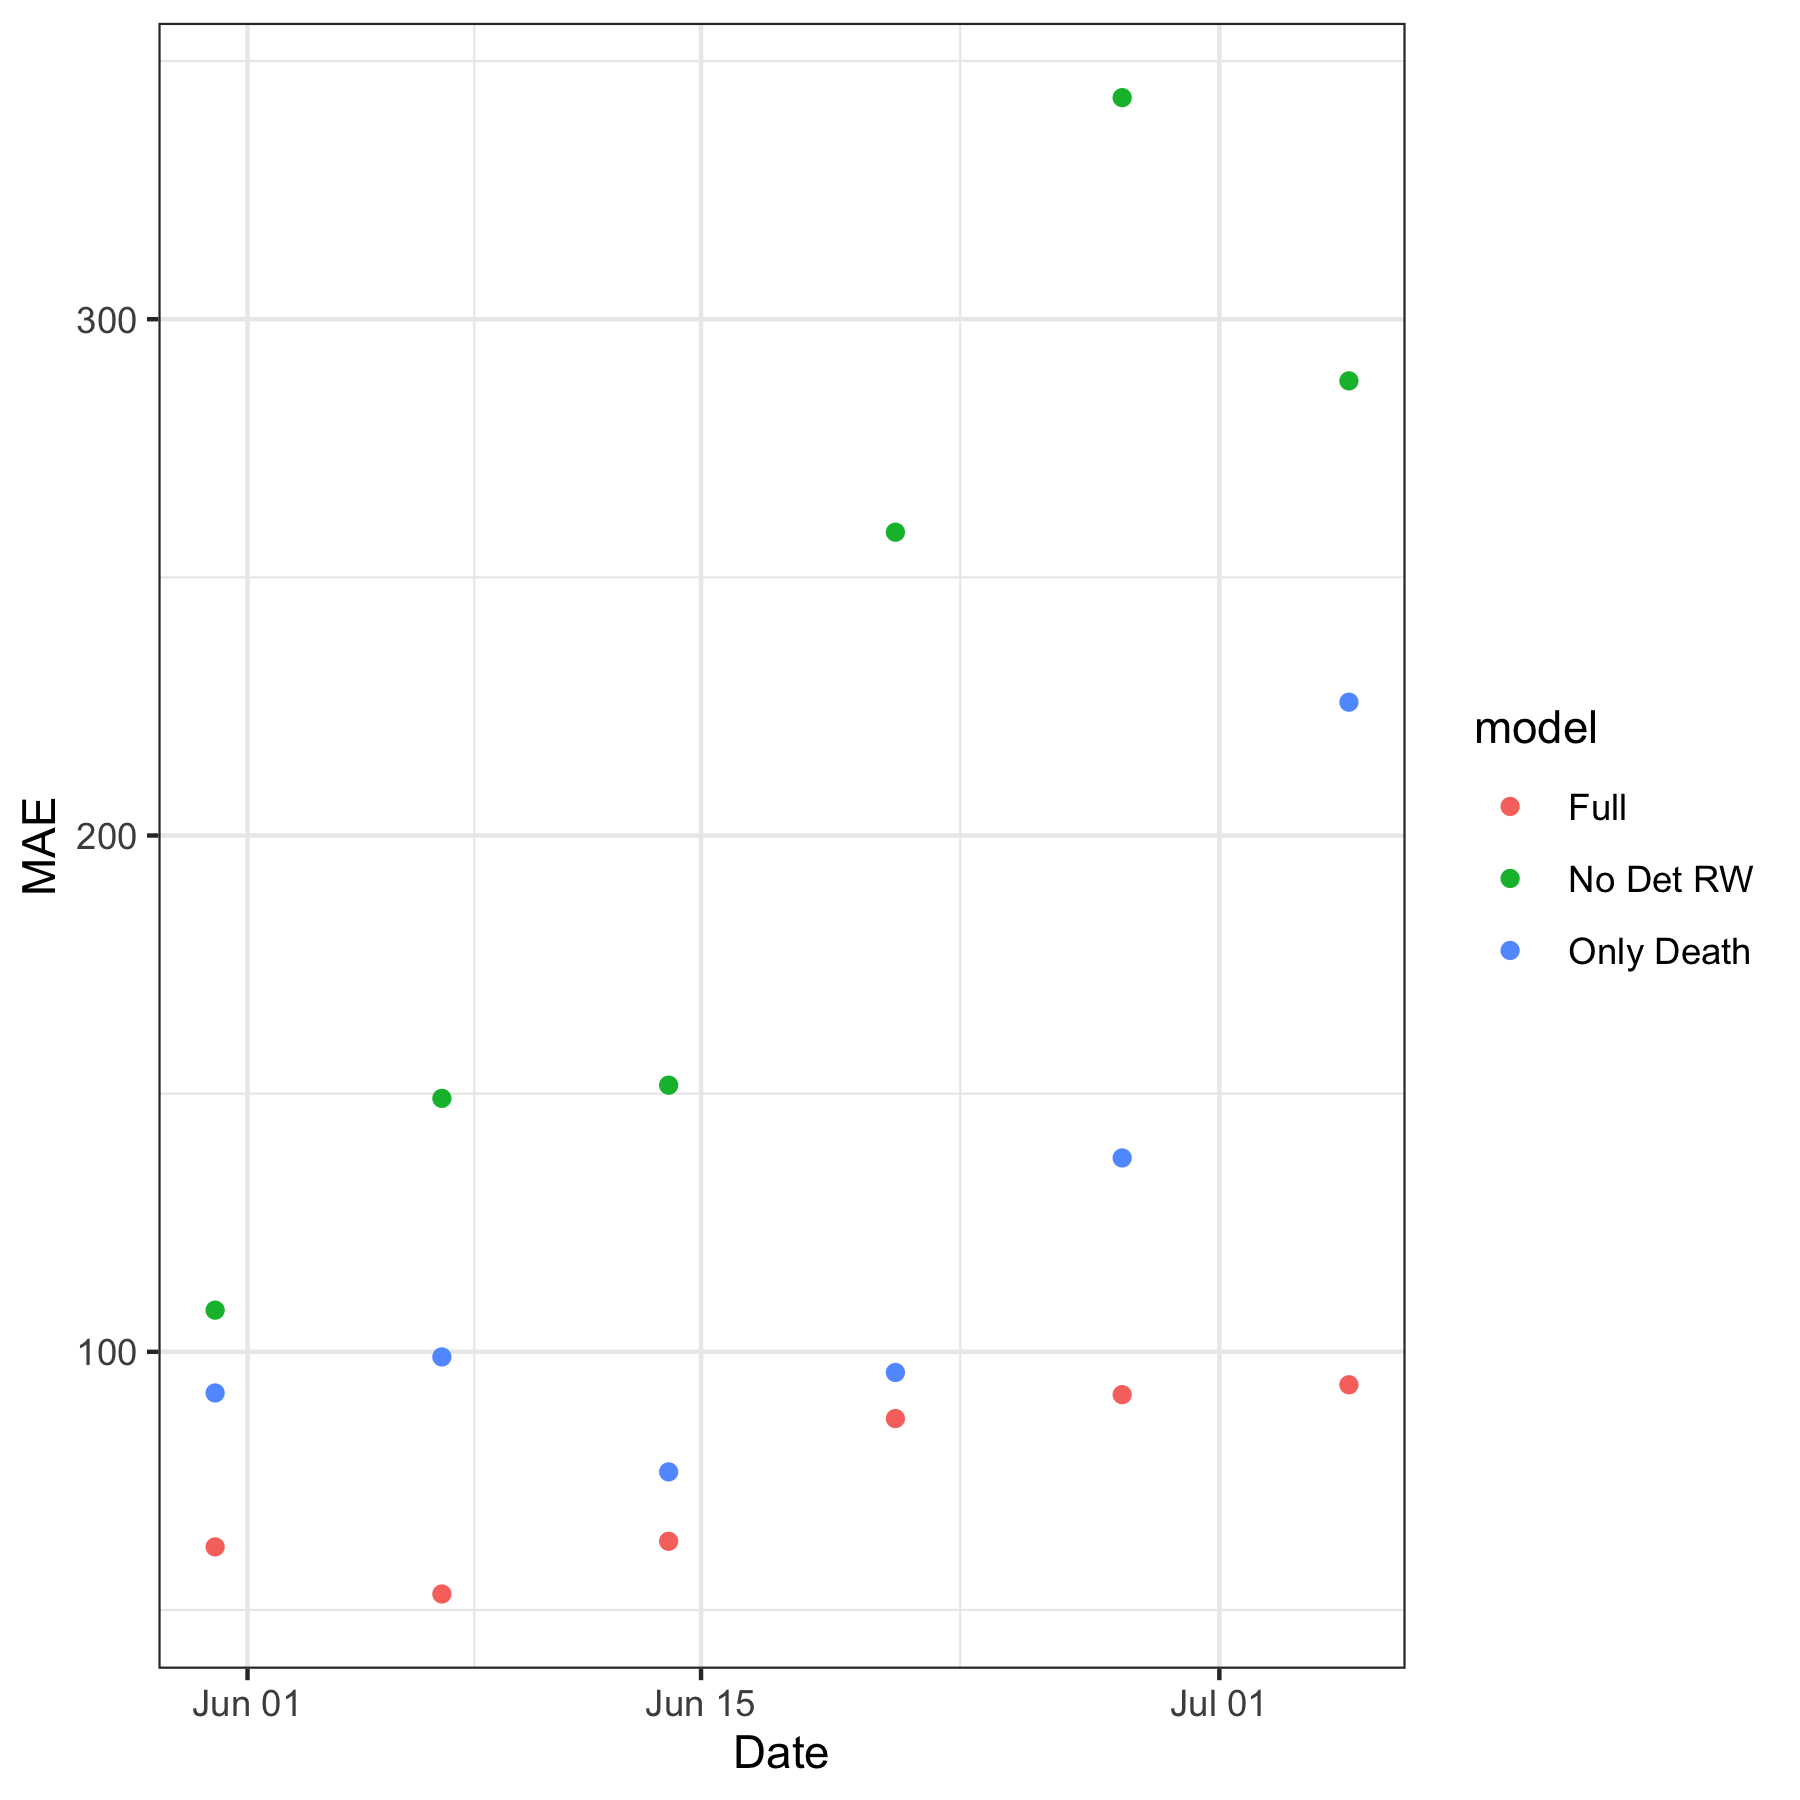
\includegraphics[scale=.15]{ablation_3.png}
    \caption{3 week ahead.}
\end{subfigure}%
\begin{subfigure}{.5\textwidth}
  \centering
    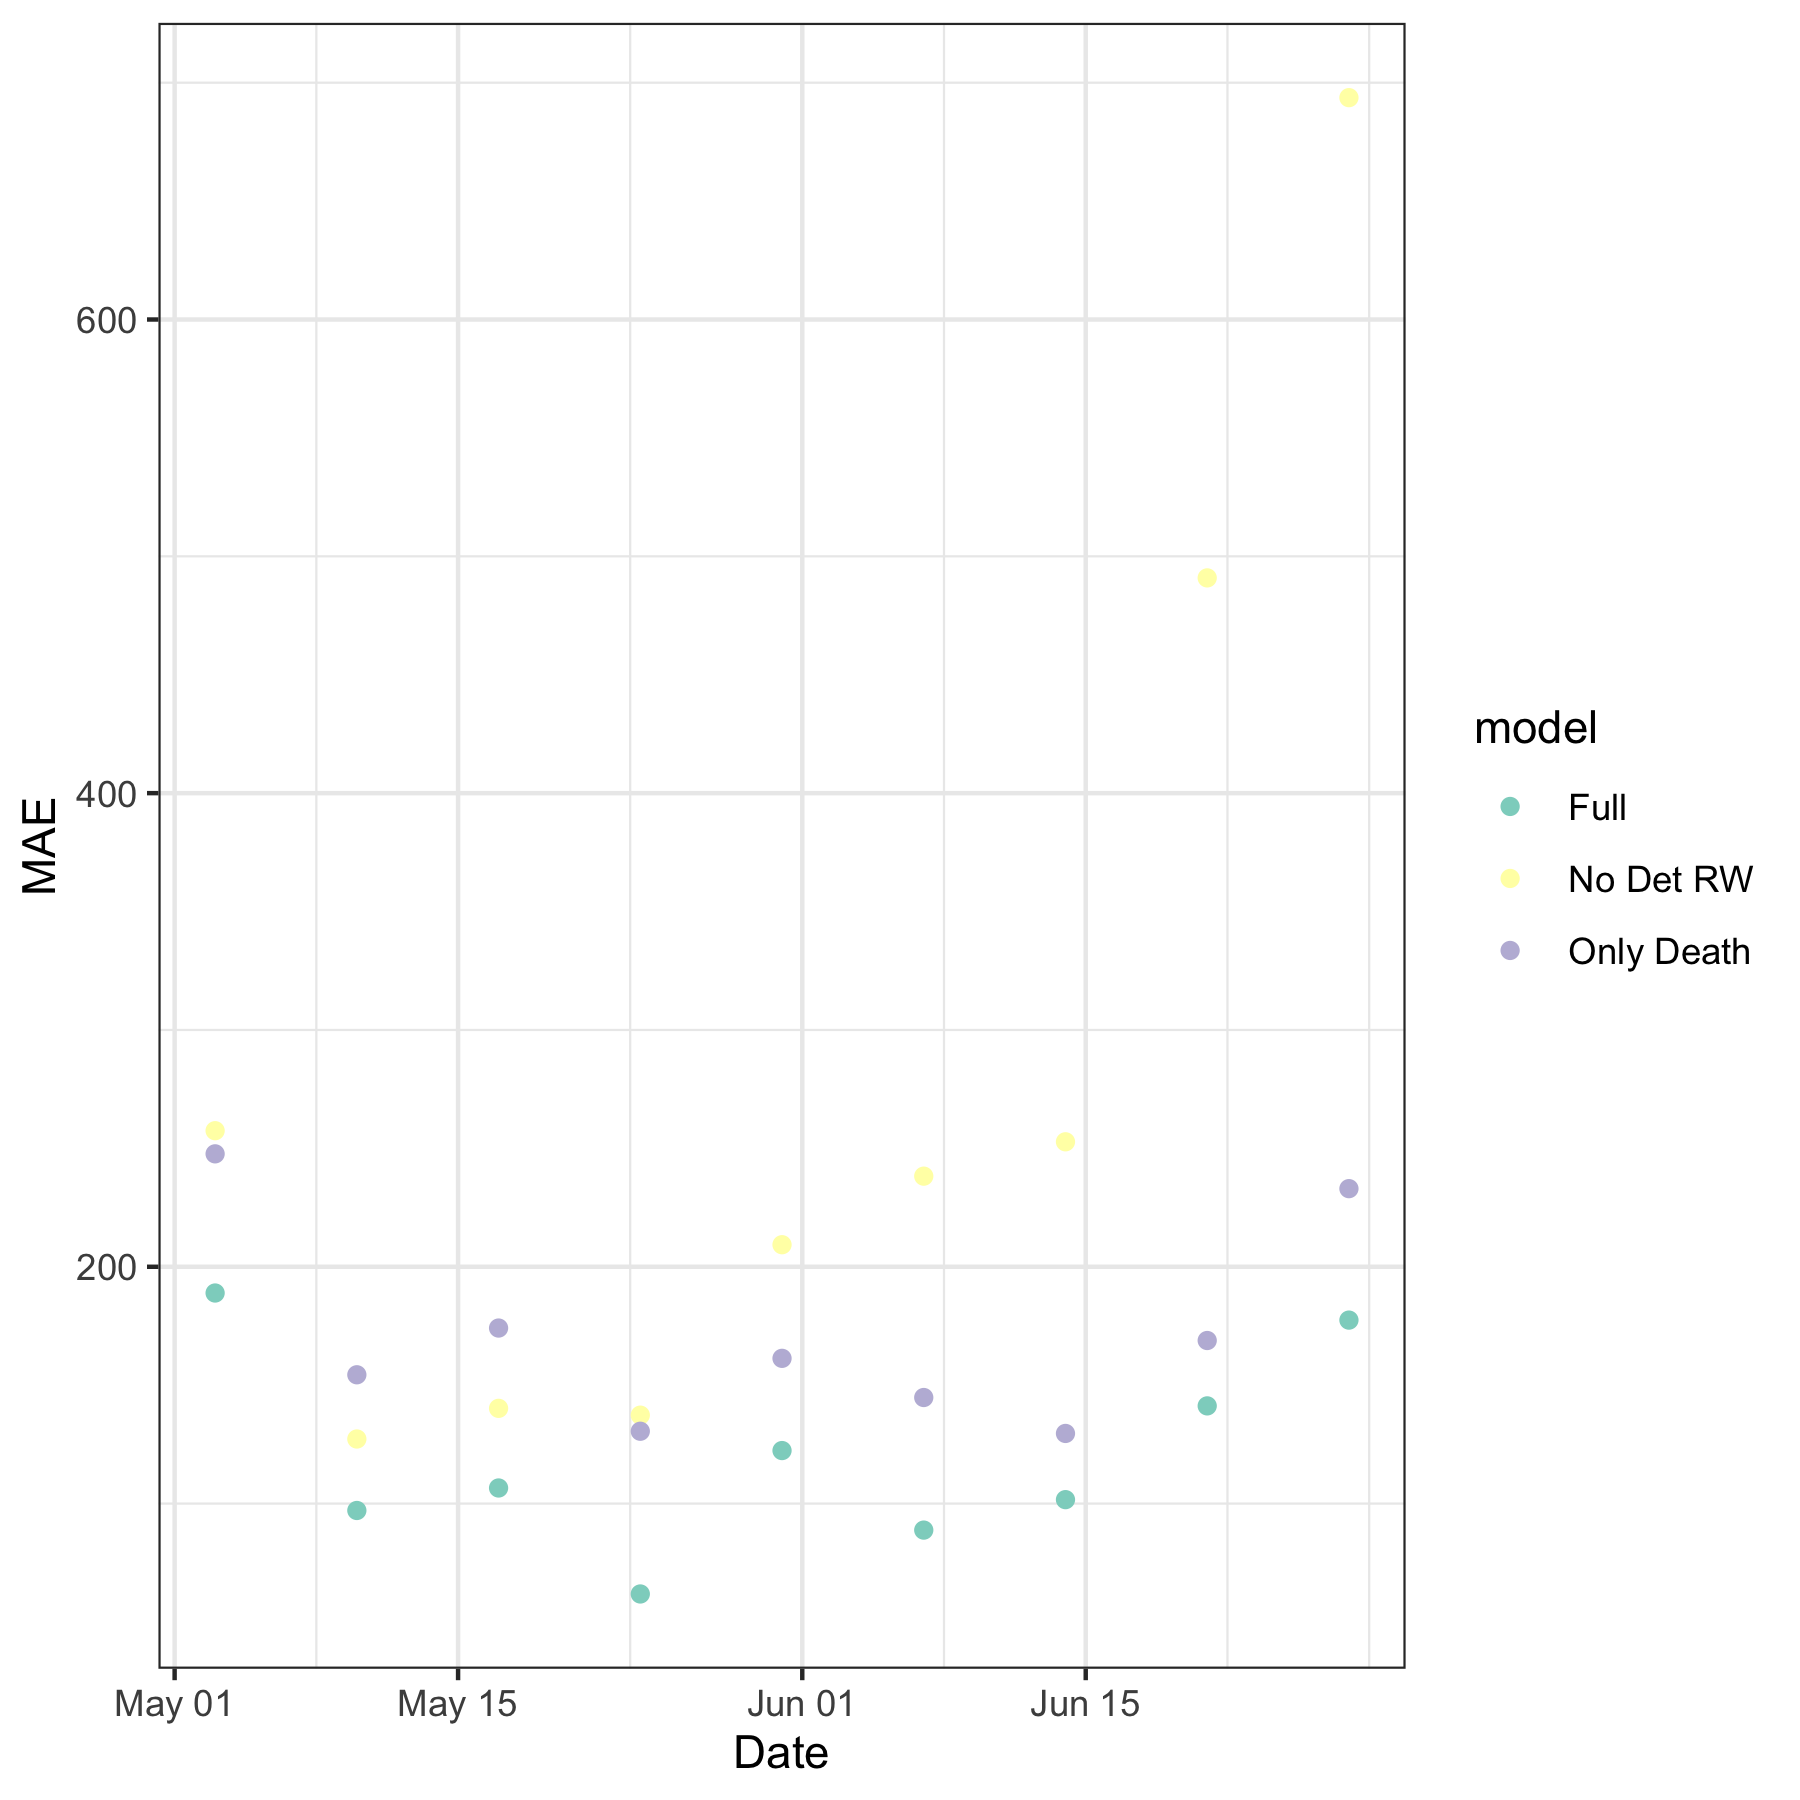
\includegraphics[scale=.15]{ablation_4.png}
    \caption{4 week ahead. }
\end{subfigure}

\caption{Ablation test MAE broken down by forecast week and target. We can see that MechBayes Case/Death Time-Varying performs better than MechBayes Case/Death Fxied and MechBayes Death Fixed in almost all breakdowns. We can also see that the improvement becomes more pronounced at larger horizons, suggesting that MechBayes Case/Death Time-Varying is a better longer term forecasting model.  }
\label{fig:ablation}
\end{figure}




\section{Discussion}

MechBayes is a fast, fully Bayesian compartmental model capable of accounting for real-world data challenges during a pandemic.  This model produced consistently accurate real-time forecasts over the course of 3 months, and was ranked as one of the top 3 of 11 models on an independent scoreboard of COVID-19 forecast models \cite{yyg}. Our experiments led us to the following conclusions about the performance of this model and the underlying methodology.

\begin{itemize}

\item \textbf{MechBayes is accurate when compared to a baseline model}. As Figure \ref{fig:covidhub} shows, MechBayes improved relative to the baseline model when broken down by timezero and target. The results are more pronounced when breaking down by target, where the boxplots are almost completely separated. These results are statistically significant for 1-4 weeks ahead, with larger improvements at later horizons, suggesting that the biggest improvements from MechByes over the baseline model comes in longer term forecasting. Additionally, as seen in Figure \ref{fig:covidhub_region_results} , the biggest gains in performance in MAE occur in regions with the largest total deaths counts. This is a desirable feature of a pandemic forecasting model. 

\item \textbf{MechBayes is probabilistically well-calibrated}. As we can see from Figure \ref{fig:covidhub} (B,D), the coverage probability of MechBayes is much closer to 95\%. When averaging over target, region, and timezero the coverage probability is 94.6\%. This suggests that MechBayes is very well calibrated at the 95\% level. The two sources of uncertainty in MechBayes come from the distribution over the differential equation parameters and the observation noise. The model is able to learn reasonable estimates of these variance parameters to produce well calibrated results. 


\item \textbf{Adding case data when predicting deaths is helpful but only when accounting for data quality issues}. Our ablation tests (Figure \ref{fig:ablation}) shows that allowing for a time-varying case and death deviation model is a key feature for reducing MAE of forecasts. MechBayes Case/Death time-varying both incorporates incident cases into the model likelihood and allows for a flexible deviation between cases and deaths is consistently more accurate than a model that does not account for cases at all ("Death Fixed" model) and a model that does account for cases but does not account for a time-varying deviation between cases and deaths.

%As we can see in Figure \ref{fig:model_details}, the model relies on this parameter heavily, setting the case and death deviation model at around 15\% at the start of the pandemic in March, to nearly 80\% by August 1st 2020. There is remarkable similarity between the increase across geographical locations as well, suggesting (as testing data reflects) an overall increase in the number of detected cases across the U.S. Adjusting for case data quality also requires a QA process, where data dumps are redistributed across a specific time-window. This avoids the situation where MechBayes interprets data dumps as a drastic change in disease dynamics. This is visible in Figure \ref{fig:model_details}, where the time-varying case and death deviation model in New Jersey follows the typical trend of other states, until the data dump, where the case and death deviation model dips significantly down.



%*\item \textbf{MechBayes is biased high}. We can see from Figure \ref{fig:results_discussion} that MechBayes was biased high with respect to the median forecast. We suspect this is due to the inherent exponential growth of an SEIR model when the number of susceptibles is large. Since overall prevalence in any state is well below the number needed to reach herd immunity, when the model sees an increase in cases it treats this as exponential growth, which translates into exponential growth in deaths. However, in the recent forecasts the bias is consistently lower than the COVID-19 Forecast Hub baseline model. Note the extreme low bias in the first submission is due to the omission of the U.S. in the submission. Late June 2020 is when many states in the U.S. began to see an uptick in cases again, with Texas, Florida, and California seeing their largest total case counts since the beginning of the pandemic. Since MechBayes is conditional on the current level of interventions, forecasts made from June 22nd assumed the same level of intervention present on June 22nd. During this time, each state was re-opening various establishments, while cases were rising. MechBayes Case/Death Time-Varying forecasted an exponential growth in cases, which was reflected in a large over prediction two weeks later on July 4th. *%

\item \textbf{Most epidemiological parameters are unidentifiable from the data}. MechBayes requires relatively informative priors on $\sigma$, $\gamma$, $\rho$ and $\lambda$. These parameters reflect the biology of the disease, from latent incubation period to average time from symptom onset to death. Since the data used to fit MechBayes is only a time series of confirmed cases and deaths, these parameters are simply not identifiable from the data. MechBayes was built for forecasting, not inference on epidemiological parameters. However, using a Bayesian framework we can simultaneously set priors based on the literature and allow for small deviations from the prior due to variations across states. 




\item \textbf{Allowing for time-varying transmissibility is necessary to non-parametrically capture the effect of  interventions}. Our ablation test explicitly did not include a model that fixed $\beta$ across time. This is because the model would not converge without the flexibility to capture changes in transmission. While non-parametrically modeling interventions is appealing from a forecasting perspective, it does modify the philosophy behind compartmental modeling. By including such a flexible parameter, we may view MechBayes as simply a random-walk model, with a set of epidemiological parameters transforming that random-walk in an almost deterministic way to match both cases and deaths. For instance, if the variance of the random walk $\sigma_{\beta}^2$ was allowed to be arbitrarily large, then $\beta(t)$ could vary enough to match the data exactly. This would clearly attribute reporting issues as true changes in transmissibility. Bypassing the epidemiological interpretation that compartmental models provide. 

\end{itemize}




%\begin{figure}
%\centering
%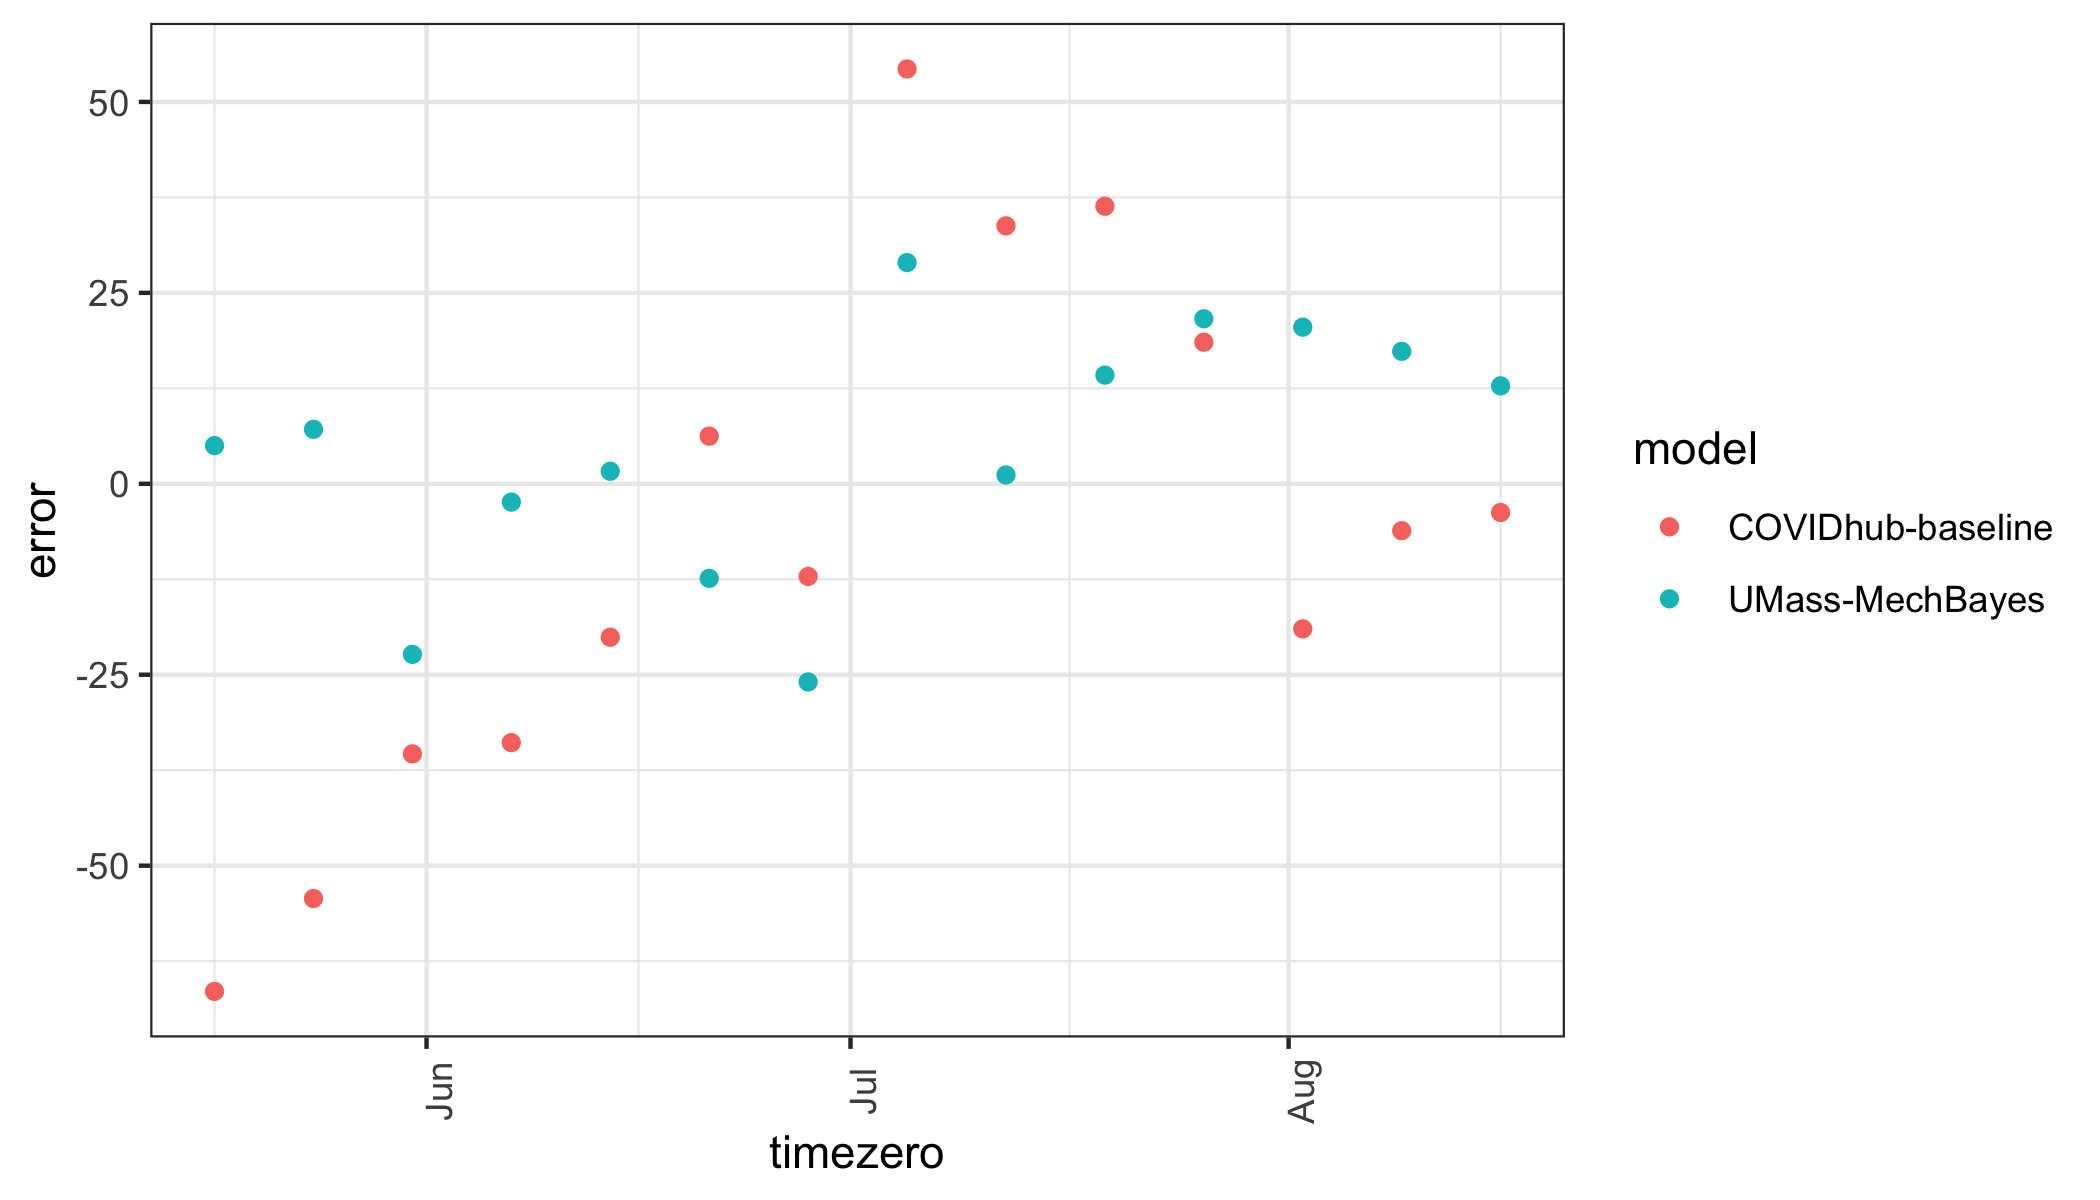
\includegraphics[scale=.15]{bias_by_timezero.png}
%\caption{Bias of MechBayes and COVID-Baseline as a function of time.  }
%\label{fig:results_discussion}
%\end{figure}



\section{Conclusion}

We have seen that MechBayes is a powerful Bayesian compartmental model that can capture the real-world complexities of forecasting during a pandemic. Through real-time and retrospective evaluation, we have demonstrated the success of MechBayes in forecasting COVID-19. The model is able to improve over a naive baseline model as well as a naive compartmental model. Allowing for time-varying interventions and case and death deviation model is a necessary model component during a real-time pandemic forecasting effort. 

While we chose an exponential random walk on $\beta(t)$ there are many other choices for flexible non-parametric modeling of transmissibility. Further work might consider a spline model, or a Gaussian process, or semi-parametric models capable of taking intervention dates as covariates. 

However, using relatively simple non-parametric methods we were able to beat a baseline model in both point and probabilistic forecast evaluations. Our ablation tests show that extending the basic SEIR compartmental to real-world pandemic challenges improves forecasting accuracy. 


\newpage

\section{Appendix}
\subsection{Statistical Test for Significance}
In order to do this, we just a random effects regression model of the form,

\begin{eqnarray*}
log(MAE_{m,t,r,h} +1) &=& \beta_0 +  \beta1*h_1 + ....+ \beta_3*h_3 \\
&+& \beta_4 *h_1*mb + .... \beta_8*h_4*mb\\
 &+& b_{r} + \epsilon \\
b_{r} &\sim &N(0,\Sigma_b^2)\\
\epsilon &\sim& N(0,\sigma^2)
\end{eqnarray*}

where $mb$ is an indicator for the MechBayes model, $t$ is timezero, $r$ is region, and $h$ is target horizon (1-4 week ahead). We chose this model because it explains the variation in MAE by model and horizon while allowing varying baseline MAE values by region. Here, variation over time in MAE within a specific region is explained by differences in model performance This leads to the following coefficient estimates for the fixed effects.

\begin{table}[ht]
\centering
\begin{tabular}{rrrrrr}
  \hline
 & Estimate & Std. Error & df & t value & Pr($>$$|$t$|$) \\ 
  \hline
$\beta_0$  & 2.47 & 0.17 & 54.87 & 14.97 & 0.00 \\ 
   $\beta_{h_1}$ & 0.30 & 0.06 & 4643.00 & 5.18 & 0.00 \\ 
 $\beta_{h_2} $ & 0.44 & 0.06 & 4643.00 & 7.56 & 0.00 \\ 
  $\beta_{h_3}$ & 0.59 & 0.06 & 4643.00 & 9.79 & 0.00 \\ 
  $\beta_{h_1 mb}$  & -0.19 & 0.06 & 4643.00 & -3.19 & 0.00 \\ 
  $\beta_{h_2 mb}$ & -0.29 & 0.06 & 4643.00 & -4.87 & 0.00 \\ 
   $\beta_{h_3mb}$ & -0.23 & 0.06 & 4643.00 & -3.94 & 0.00 \\ 
 $\beta_{h_4mb}$ & -0.29 & 0.06 & 4643.00 & -4.72 & 0.00 \\ 
   \hline
\end{tabular}
\caption{Coefficient estimates and t-values for MAE evaluation model. We can see that MechBayes performs statistically significantly better than the baseline model for 1-4 weeks ahead. The performance increase seems to grow as horizon increases.}
\end{table}


\subsection{Seeding Epidemic}
Due to the under-reporting of cases, we cannot use the observed data to seed the epidemic. We instead allow the model to find the initial state values for all compartments except the number of susceptible people, which we take as the population size of the geographic region minus the sum of the initial values for the other compartments to enforce the constraint that the entire system size sums to the population size. We do this by assigning uniform probability to all initial states where the number of people in any given compartment at time zero does not exceed 2\% of the total population. This is a highly conservative estimate for the number of infected, exposed, dead and recovered people at the start of the epidemic which is most likely much lower than 2\% of the population. 

\begin{align*}
 E_0 &\sim \Unif(0, 0.02 N) \\
I_0 &\sim \Unif(0, 0.02 N) \\
  D_{1_0} &\sim \Unif(0, 0.02 N) \\
   D_{2_0} &\sim \Unif(0, 0.02 N) \\   
   R_{0} &\sim \Unif(0, 0.02 N) \\   
\end{align*}

This allows us to initialize the process model:
 \begin{equation} 
 X(0) = (S(0), E(0), I(0), R(0), D_1(0), D_2(0), C(0)) = (N-E_0-I_0-D_{1_0}-D_{2_0},E_0,I_0, R_0, D_{1_0}, D_{2_0}, I_0)
 \end{equation}
%
% \begin{itemize}
% \item Because of case and death deviation model we cannot seed using initial reported data, since this is an underestimate
% \item Put priors on initial seed
%  \end{itemize}
  
  \subsection{Priors}
We also place the following priors on the transition parameters: 
\begin{align*}
\sigma &\sim \Gamma(5, 5 \hat{d}_E)\\
\gamma & \sim \Gamma(7, 7 \hat{d}_I) \\
\beta(0) &\sim \Gamma(1, \hat{d}_I/\hat{R}) \\
    \rho &\sim \Beta(10, 90)\\ 
\lambda &\sim \Gamma(10, 100)
\end{align*}
 Our prior on rate for leaving the exposed compartment $\sigma$ satisfies $\E[\sigma] = 1/\hat{d}_E$, where $\hat{d}_E$ is an initial guess of the duration of the latent period. Currently, we assume $\hat{d}_E = 4.0$ based on published estimates (shortened slightly to account for possible infectiousness prior to developing symptoms) \cite{midas}.
 %
 Our prior on the rate for leaving the infectious compartment $\gamma$ satisfies $\E[\gamma] = 1/\hat{d}_I$, where $\hat{d}_I$ is an initial guess for the duration of infectiousness. The current setting is $\hat{d}_I = 2.0$ to model the likely isolation of individuals after symptom onset \cite{heffner2020emotional}. 
Our prior on the initial transmission rate is derived from the relationship between the basic reproductive number $R(0)$ and the length of the infectious period: $R(0) = \beta(0)/\gamma = \beta(0)\times \hat{d}_I$. Therefore, we set our prior on the initial transmission rate to satisfy $\E[\beta(0)] = \hat{R}/\hat{d}_I$ where $\hat{R} = 3.0$ is an initial guess for $R(0)$ and $\hat{d}_I = 2.0$, as described above. 
%%
Our prior on the fatality rate $\rho$ satisfies $\E[\rho] = 0.1$ with 90\% probability of being between \[0.06,.14\].
Finally, our prior on the rate at which dying patients succumb  satisfies $\lambda$ $\E[\lambda] = 0.1$ with shape 10 corresponding to roughly 10 days in the $D_{1}$ compartment.



%\subsection{A2}
%
% 
%The COVID-19 Forecast Hub began soliciting forecasts in the beginning of April 2020 for 1-4 week ahead cumulative deaths. We began submitting the first version on April 20th 2020 and have since submitted forecasts every Monday from then until August 1st 2020. The forecasts use daily data up to and including the Sunday before submission the next Monday. The one week ahead forecast corresponds to the following Saturday, the two week ahead to the second following Saturday and so on. Our model went through three distinct iterations as we evaluated performance in real-time. 
% 
% \begin{itemize}
% 
% \item \textbf{Version 1: April 20th 2020 through May 10th 2020}. Model had normal observation noise (instead of negative binomial) and a non-time varying case and death deviation model. Model was fit to cumulative deaths and cases. 
% \begin{equation}
%\text{Cases}_{t} \sim N(p_{c}*C_{t} ,\sigma_{c}^2) \ \ \  
%\text{Deaths}_{t} \sim N(p_d*D_{2_{t}} , \sigma_d^2)
%\end{equation}
%
%  \item \textbf{Version 2: May 10th 2020 through May 24th 2020}. Model had normal observation noise (instead of negative binomial) and time varying case and death deviation model. Model was fit to cumulative deaths and cases. 
%  
%   \begin{equation}
%\text{Cases}_{t} \sim N(p_{t,c}*C_{t} ,\sigma_{c}^2) \ \ \  
%\text{Deaths}_{t} \sim N(p_d*D_{2_{t}} , \sigma_d^2)
%\end{equation}
%
%
%    \item \textbf{Version 3: May 24th 2020 through August 1st 2020}. Model had negative binomial observation noise  and time varying case and death deviation model. Model was fit to incident deaths and cases. 
%     \begin{equation}
%\text{Cases}_{t} \sim NB(p_{c,t}*[C_{t}-C_{t-1}] ,\sigma_{c}^2) \ \ \  
%\text{Deaths}_{t} \sim NB(p_d*[D_{2_{t}} - D_{2_{t-1}}] , \sigma_d^2)
%\end{equation}
%    
% \end{itemize} 
% 
% 
% These three versions highlight the complexities of forecasting during a real-time pandemic. Models evolve due to real-time evaluations by responding to the unique data collection environments of each pandemic. We use the model submissions made in real-time, under the corresponding version of the model as dated above, evaluated on both MAE and WIS for the weeks of 2020-05-05, 2020-05-10, 2020-05-17, 2020-05-24 2020-05-31, 2020-06-07, 2020-06-14, 2020-06-2, 2020-06-28, 2020-07-05, 2020-07-12, 2020-07-19, and 2020-07-26. Note that not all targets are observed at all weeks. This is due to 4 week ahead targets for weeks 2020-07-12 and beyond not being observable by 2020-08-01.
%  
% 
% These two versions highlight the complexities of forecasting during a real-time pandemic. Models evolve due to real-time evaluations by responding to the unique data collection environments of each pandemic.
%
%
%\begin{figure}
%  \centering
%     \begin{subfigure}{.5\textwidth}
%  \centering
%    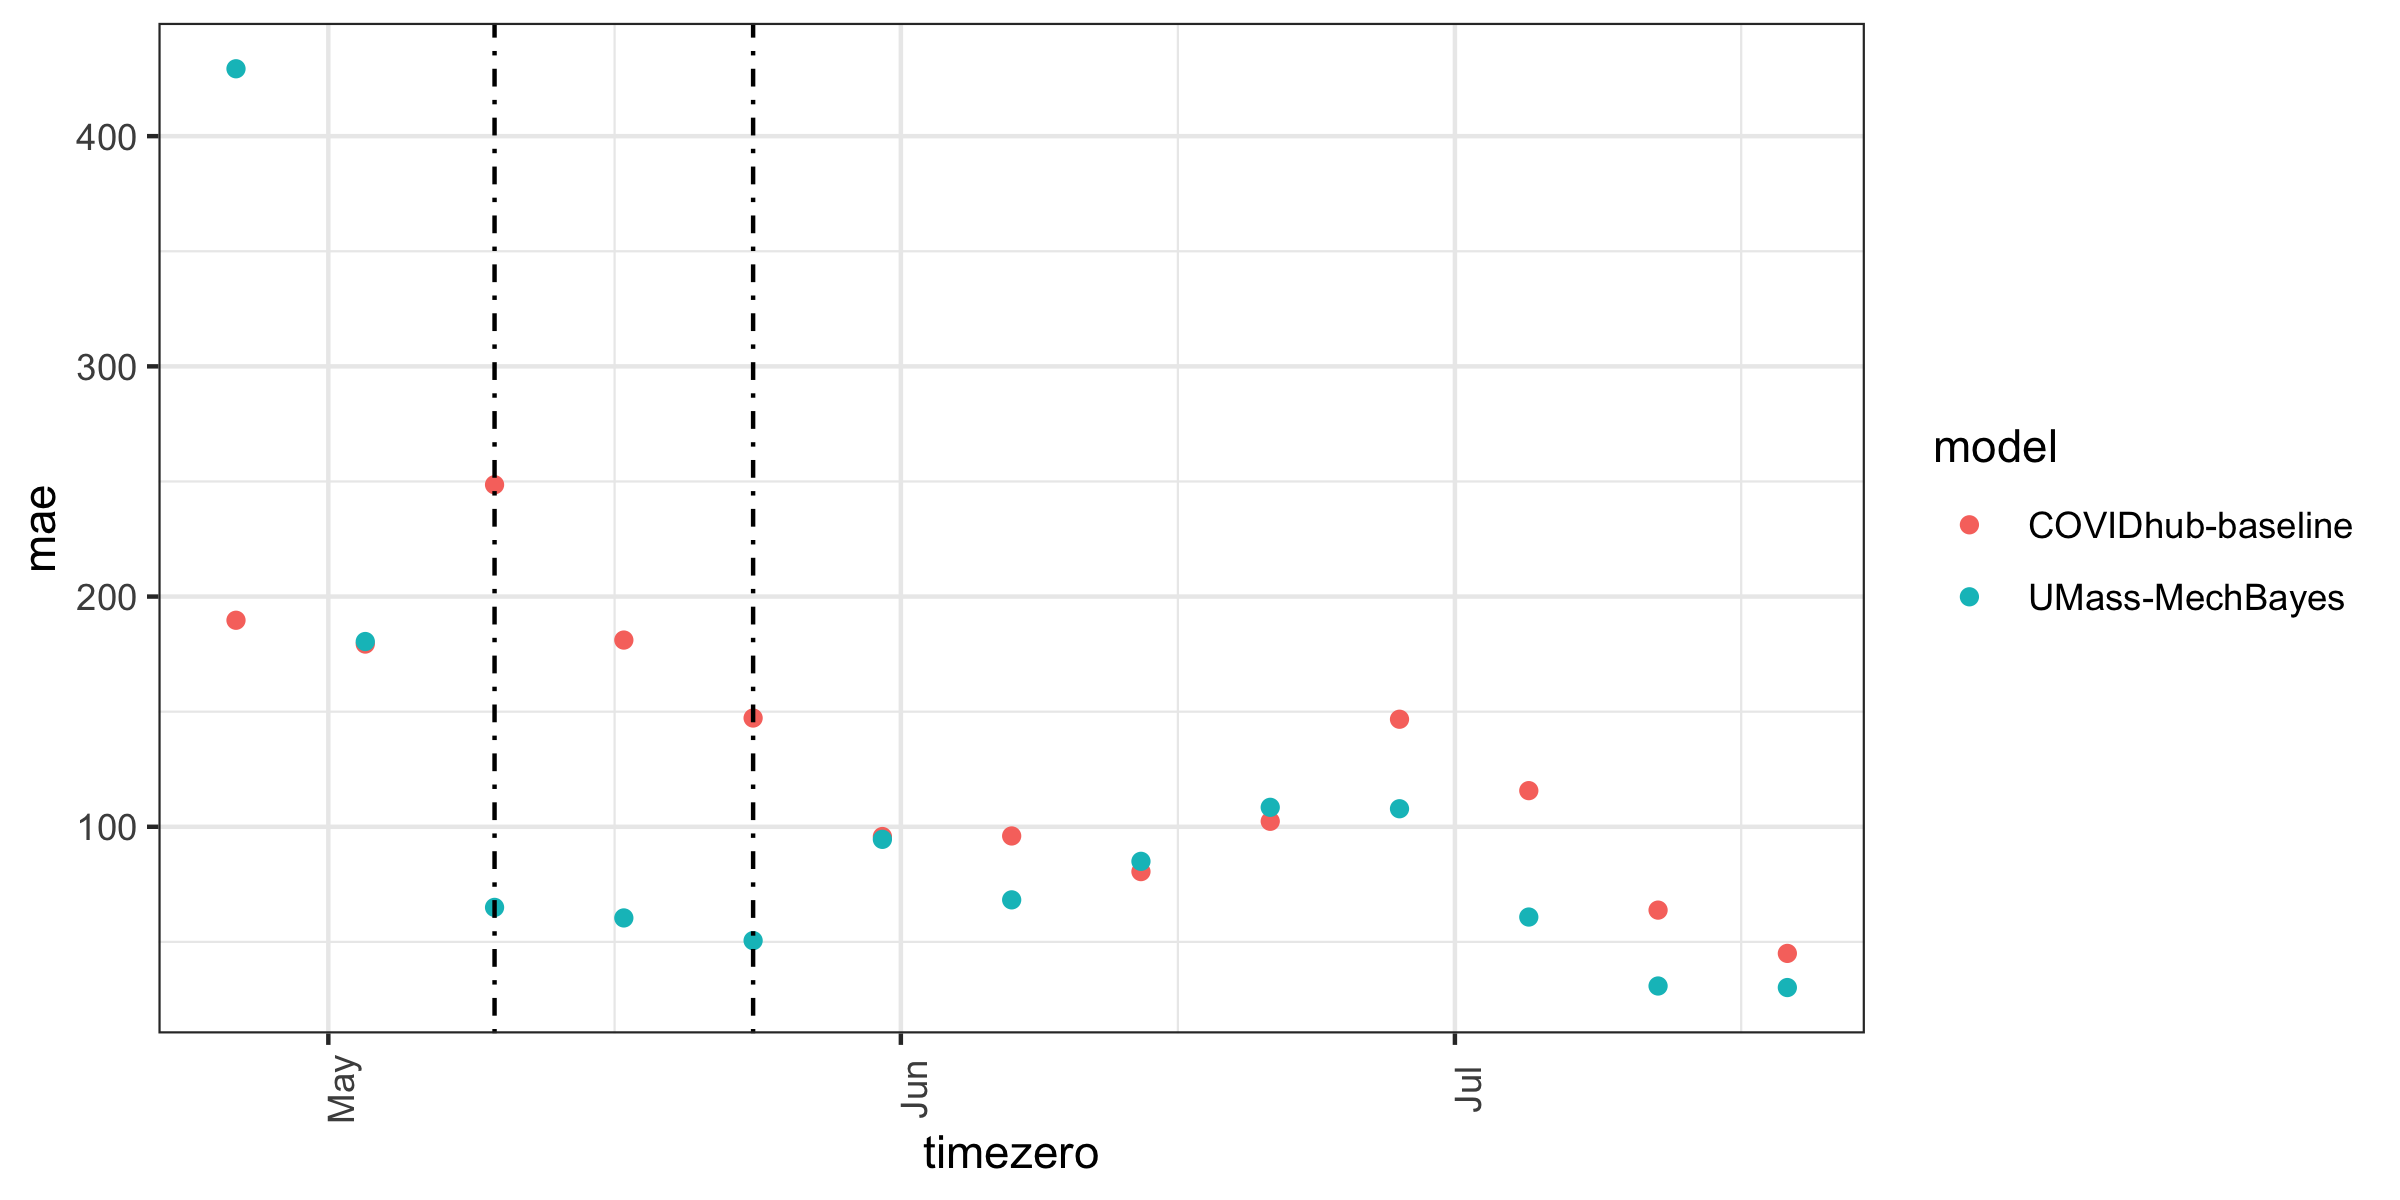
\includegraphics[scale=.1]{mae_results_by_time_zero.png}
%    \caption{MAE by forecast week}
%\end{subfigure}%
%\begin{subfigure}{.5\textwidth}
%  \centering
%    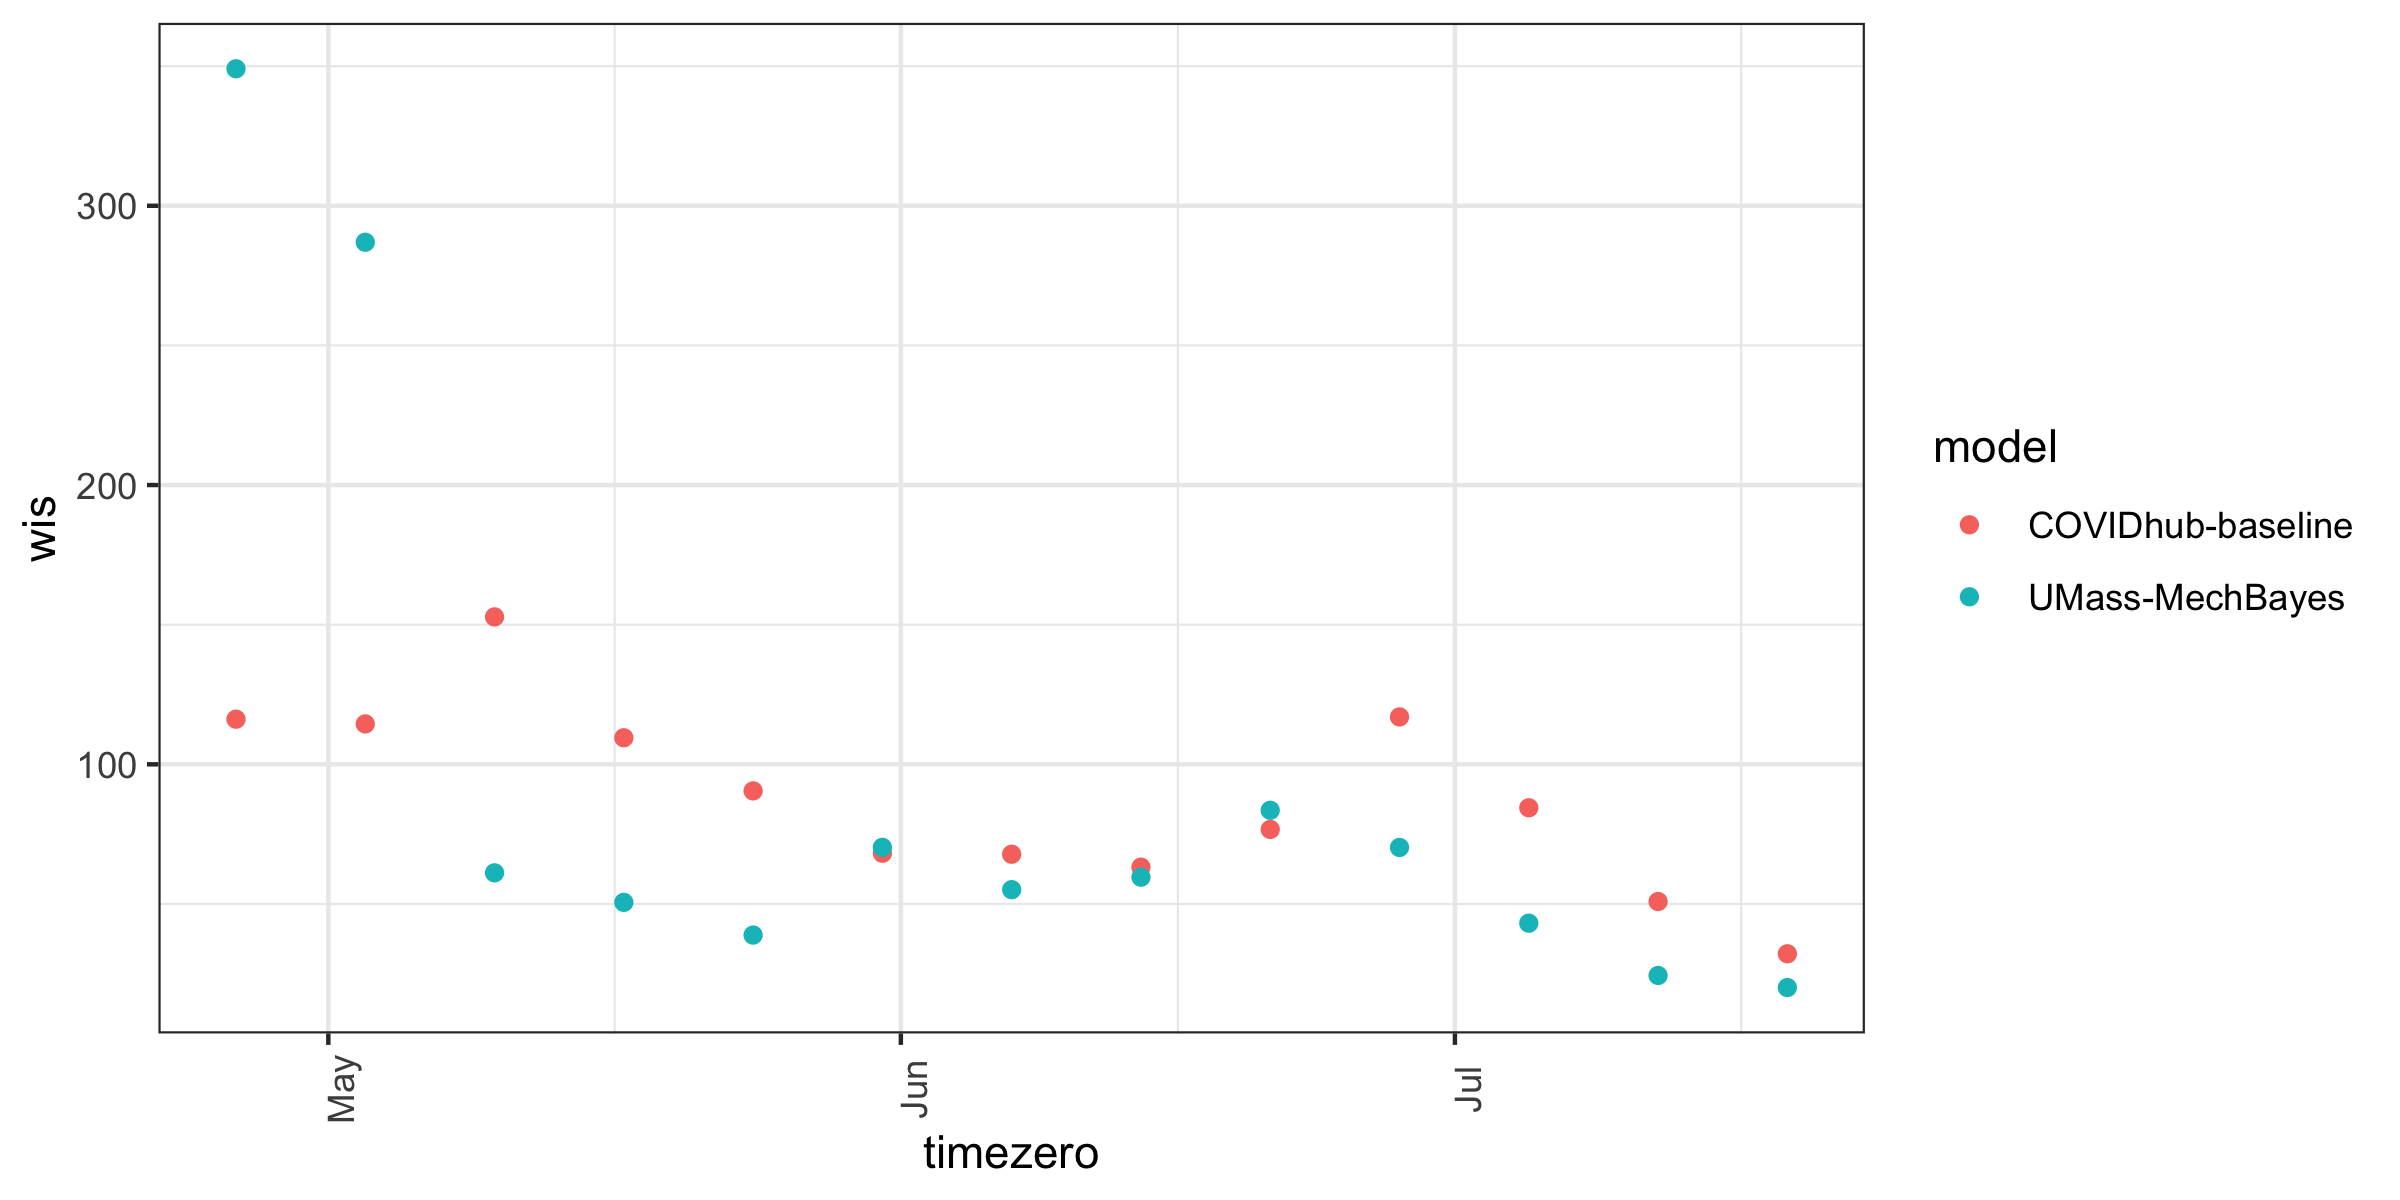
\includegraphics[scale=.1]{wis_results_by_time_zero.png}
%    \caption{WIS by forecast week}
%\end{subfigure}
%\begin{subfigure}{.5\textwidth}
%  \centering
%    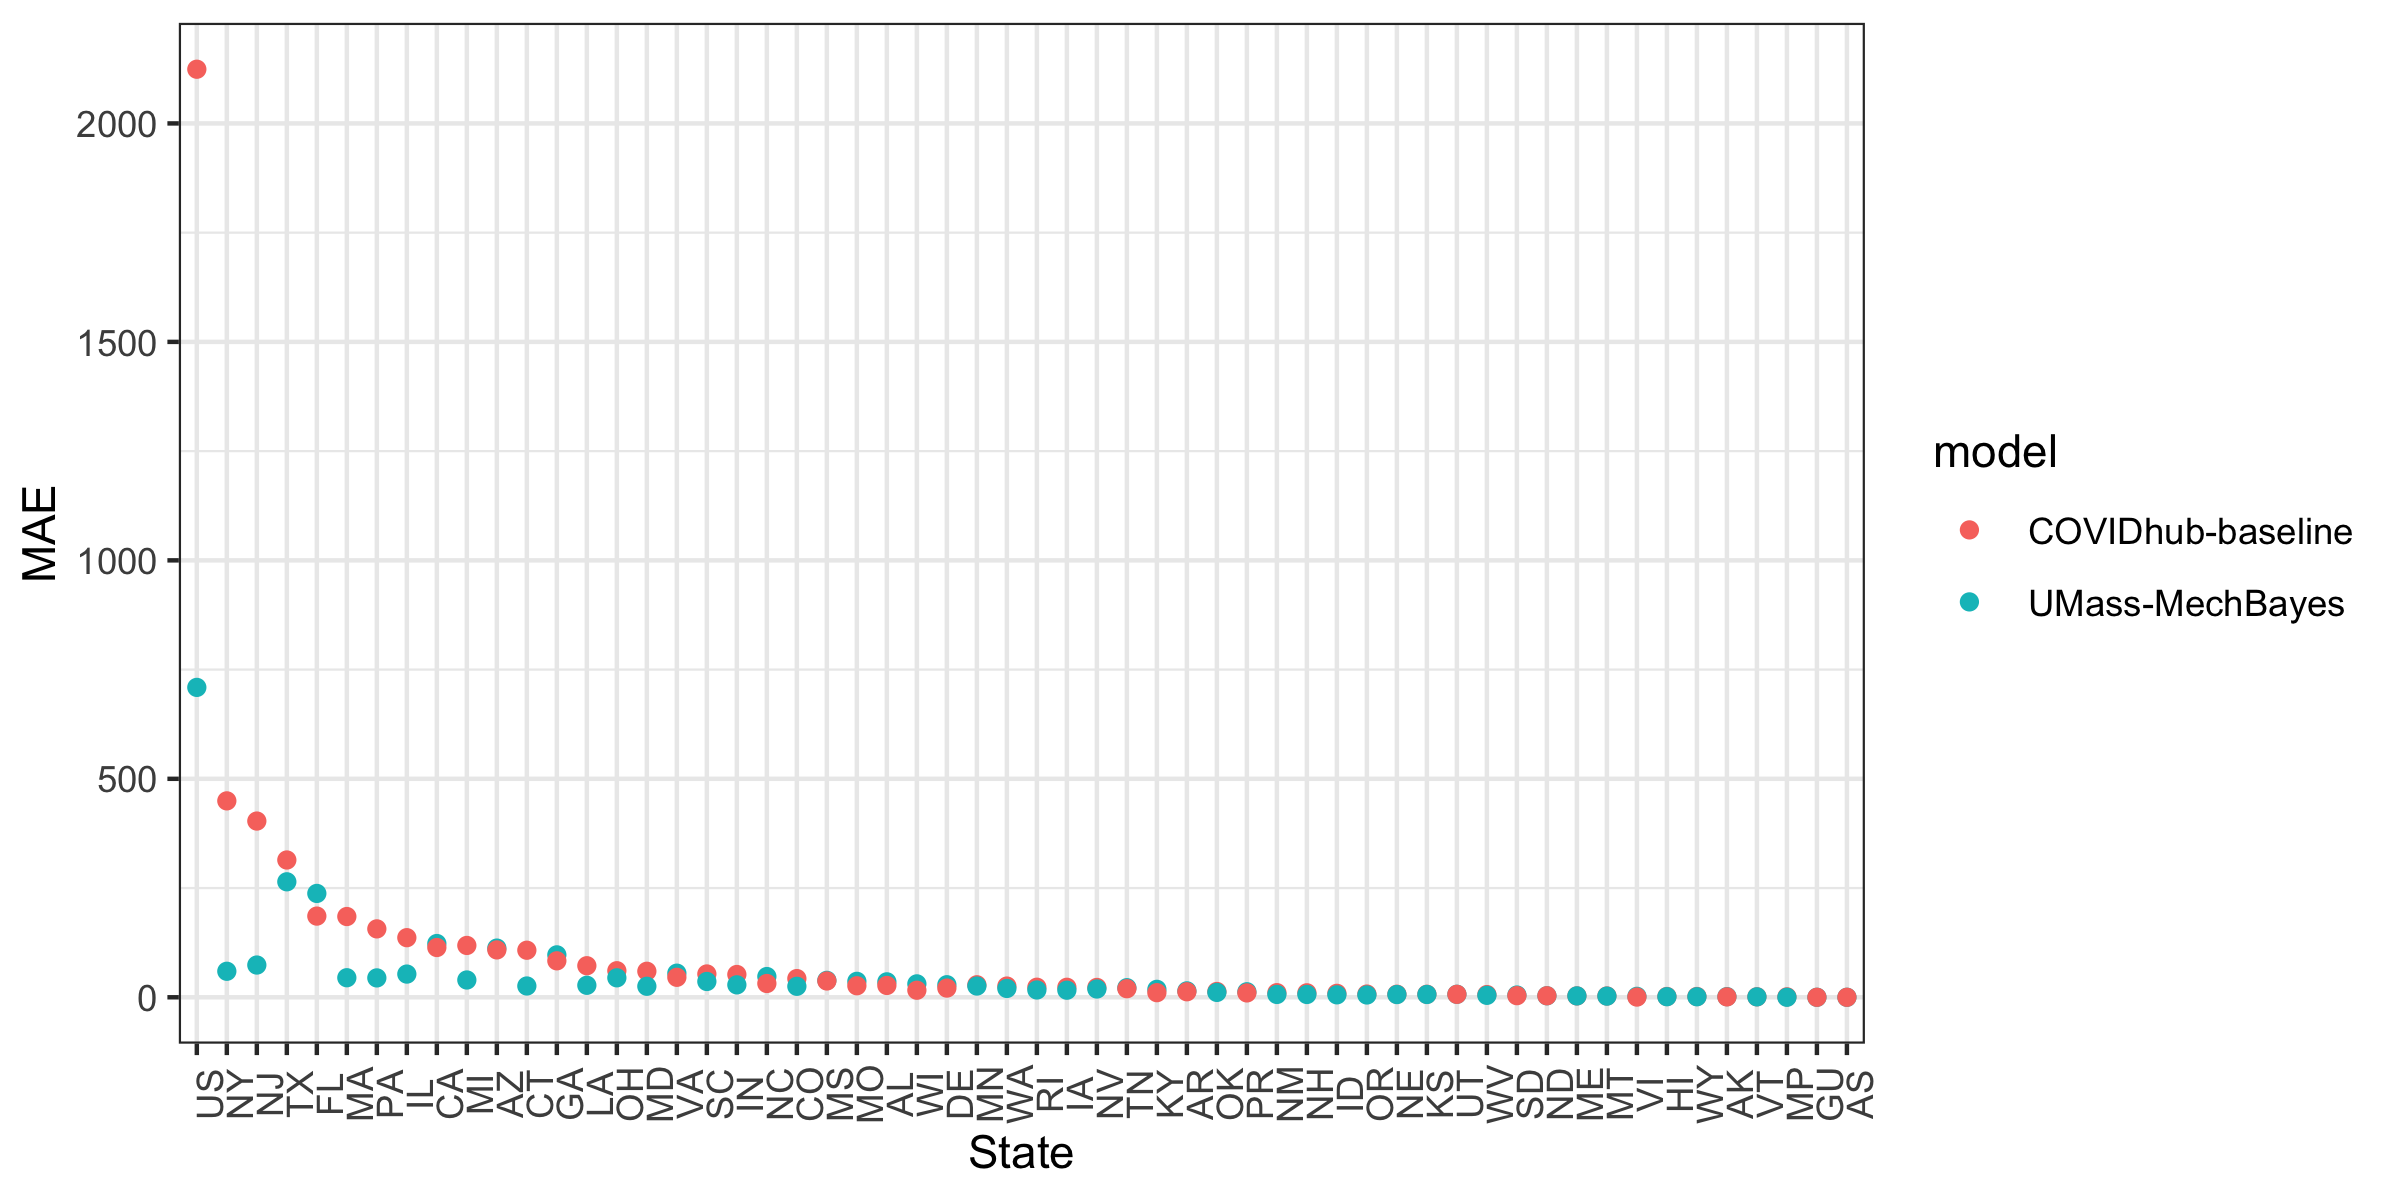
\includegraphics[scale=.1]{mae_results_by_region.png}
%    \caption{MAE by region}
%\end{subfigure}%
%\begin{subfigure}{.5\textwidth}
%  \centering
%    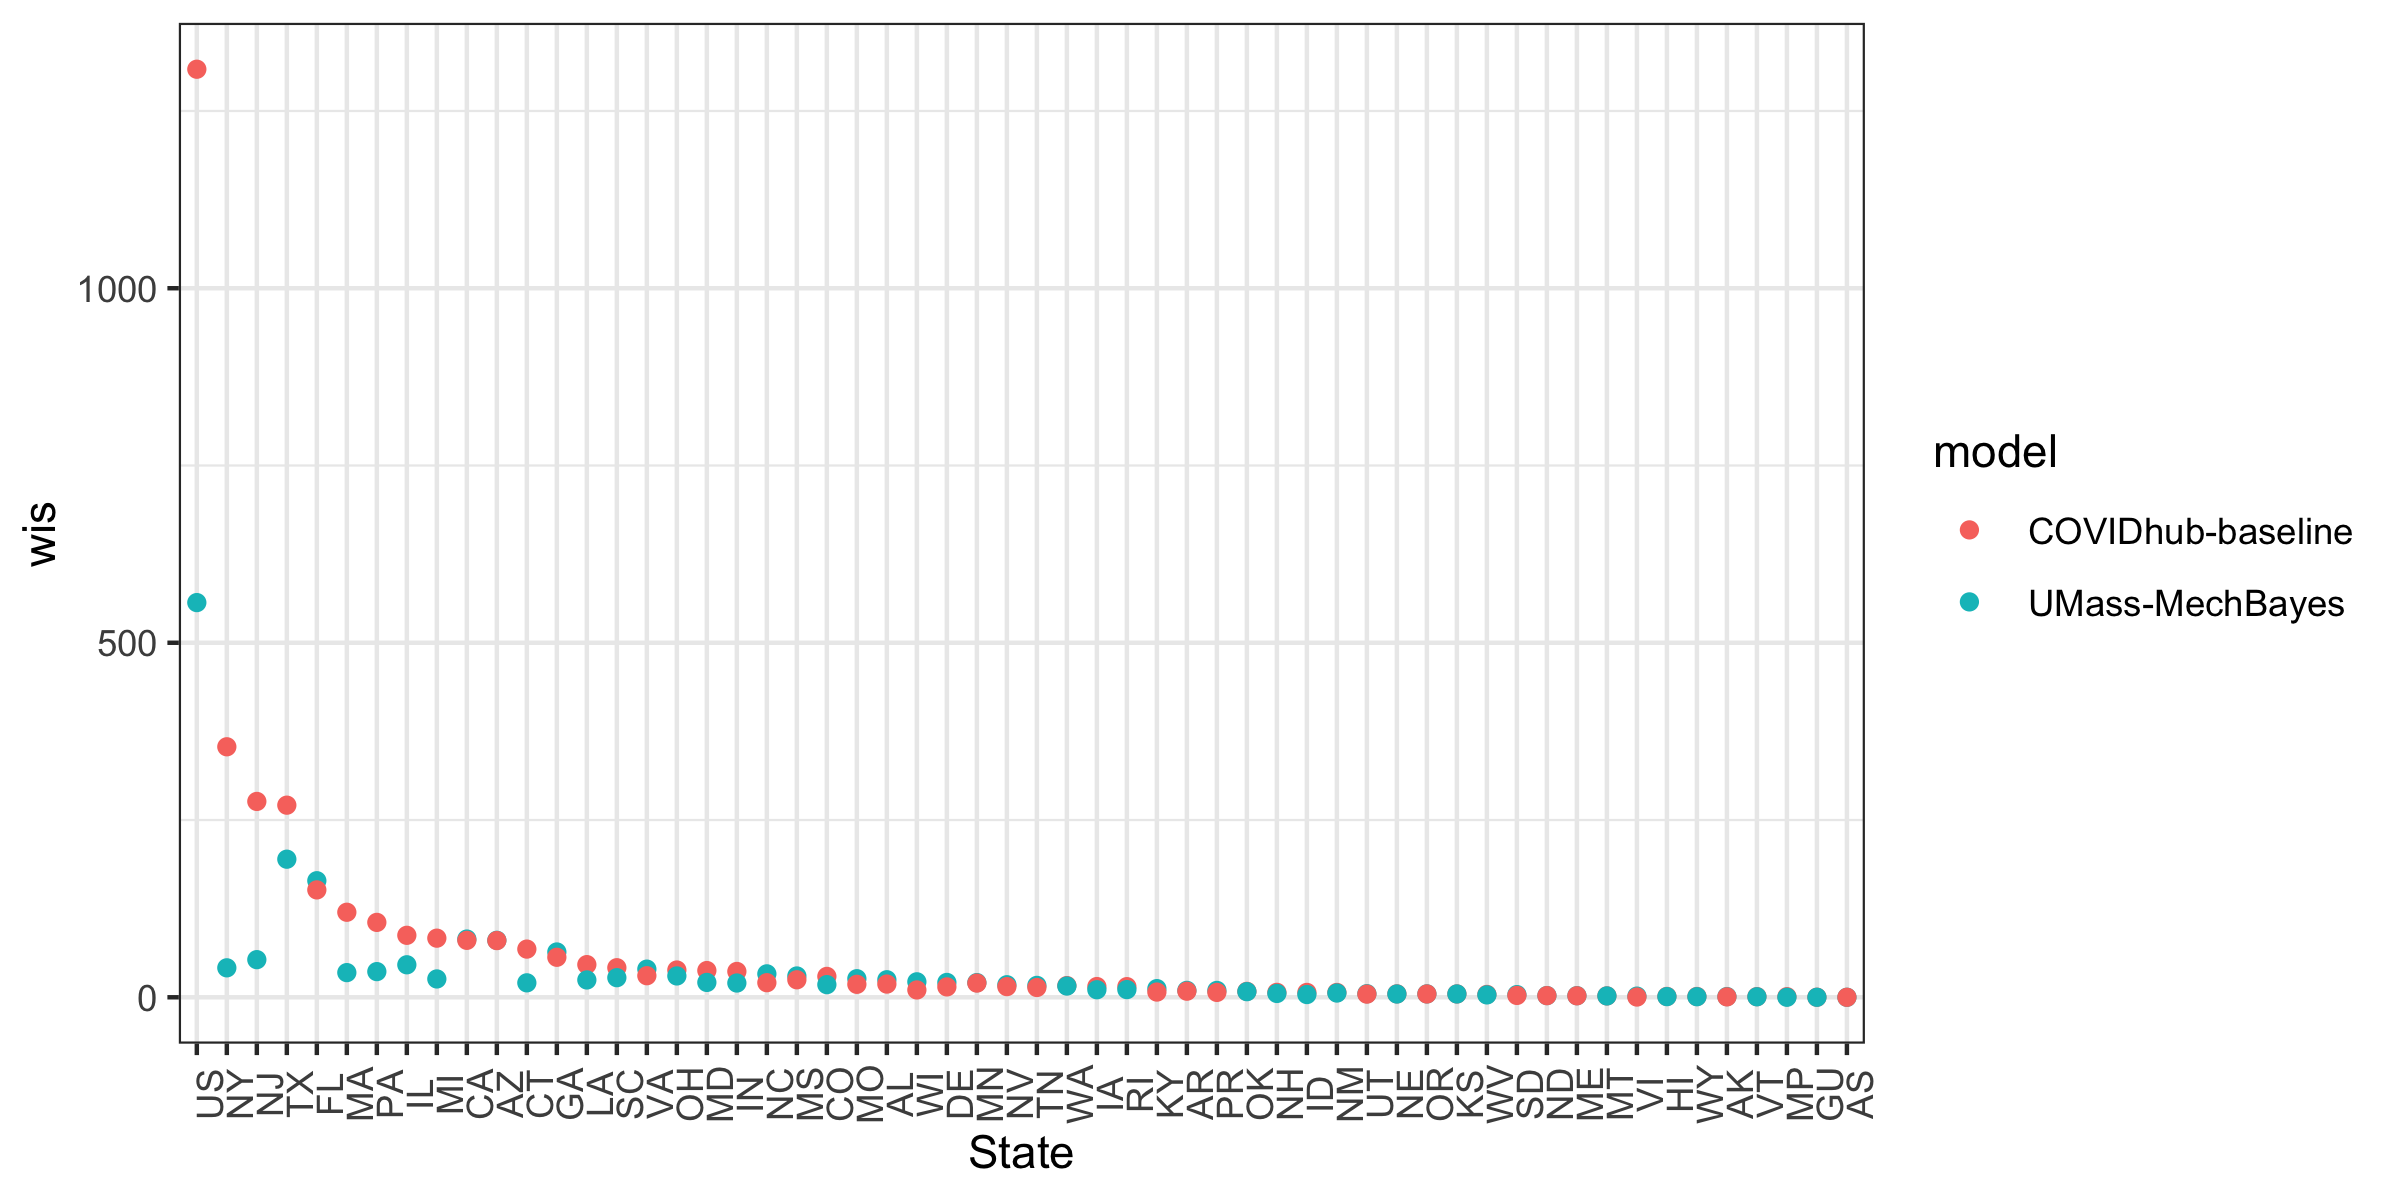
\includegraphics[scale=.1]{wis_results_by_region.png}
%    \caption{WIS by region}
%\end{subfigure}
%\begin{subfigure}{.5\textwidth}
%  \centering
%    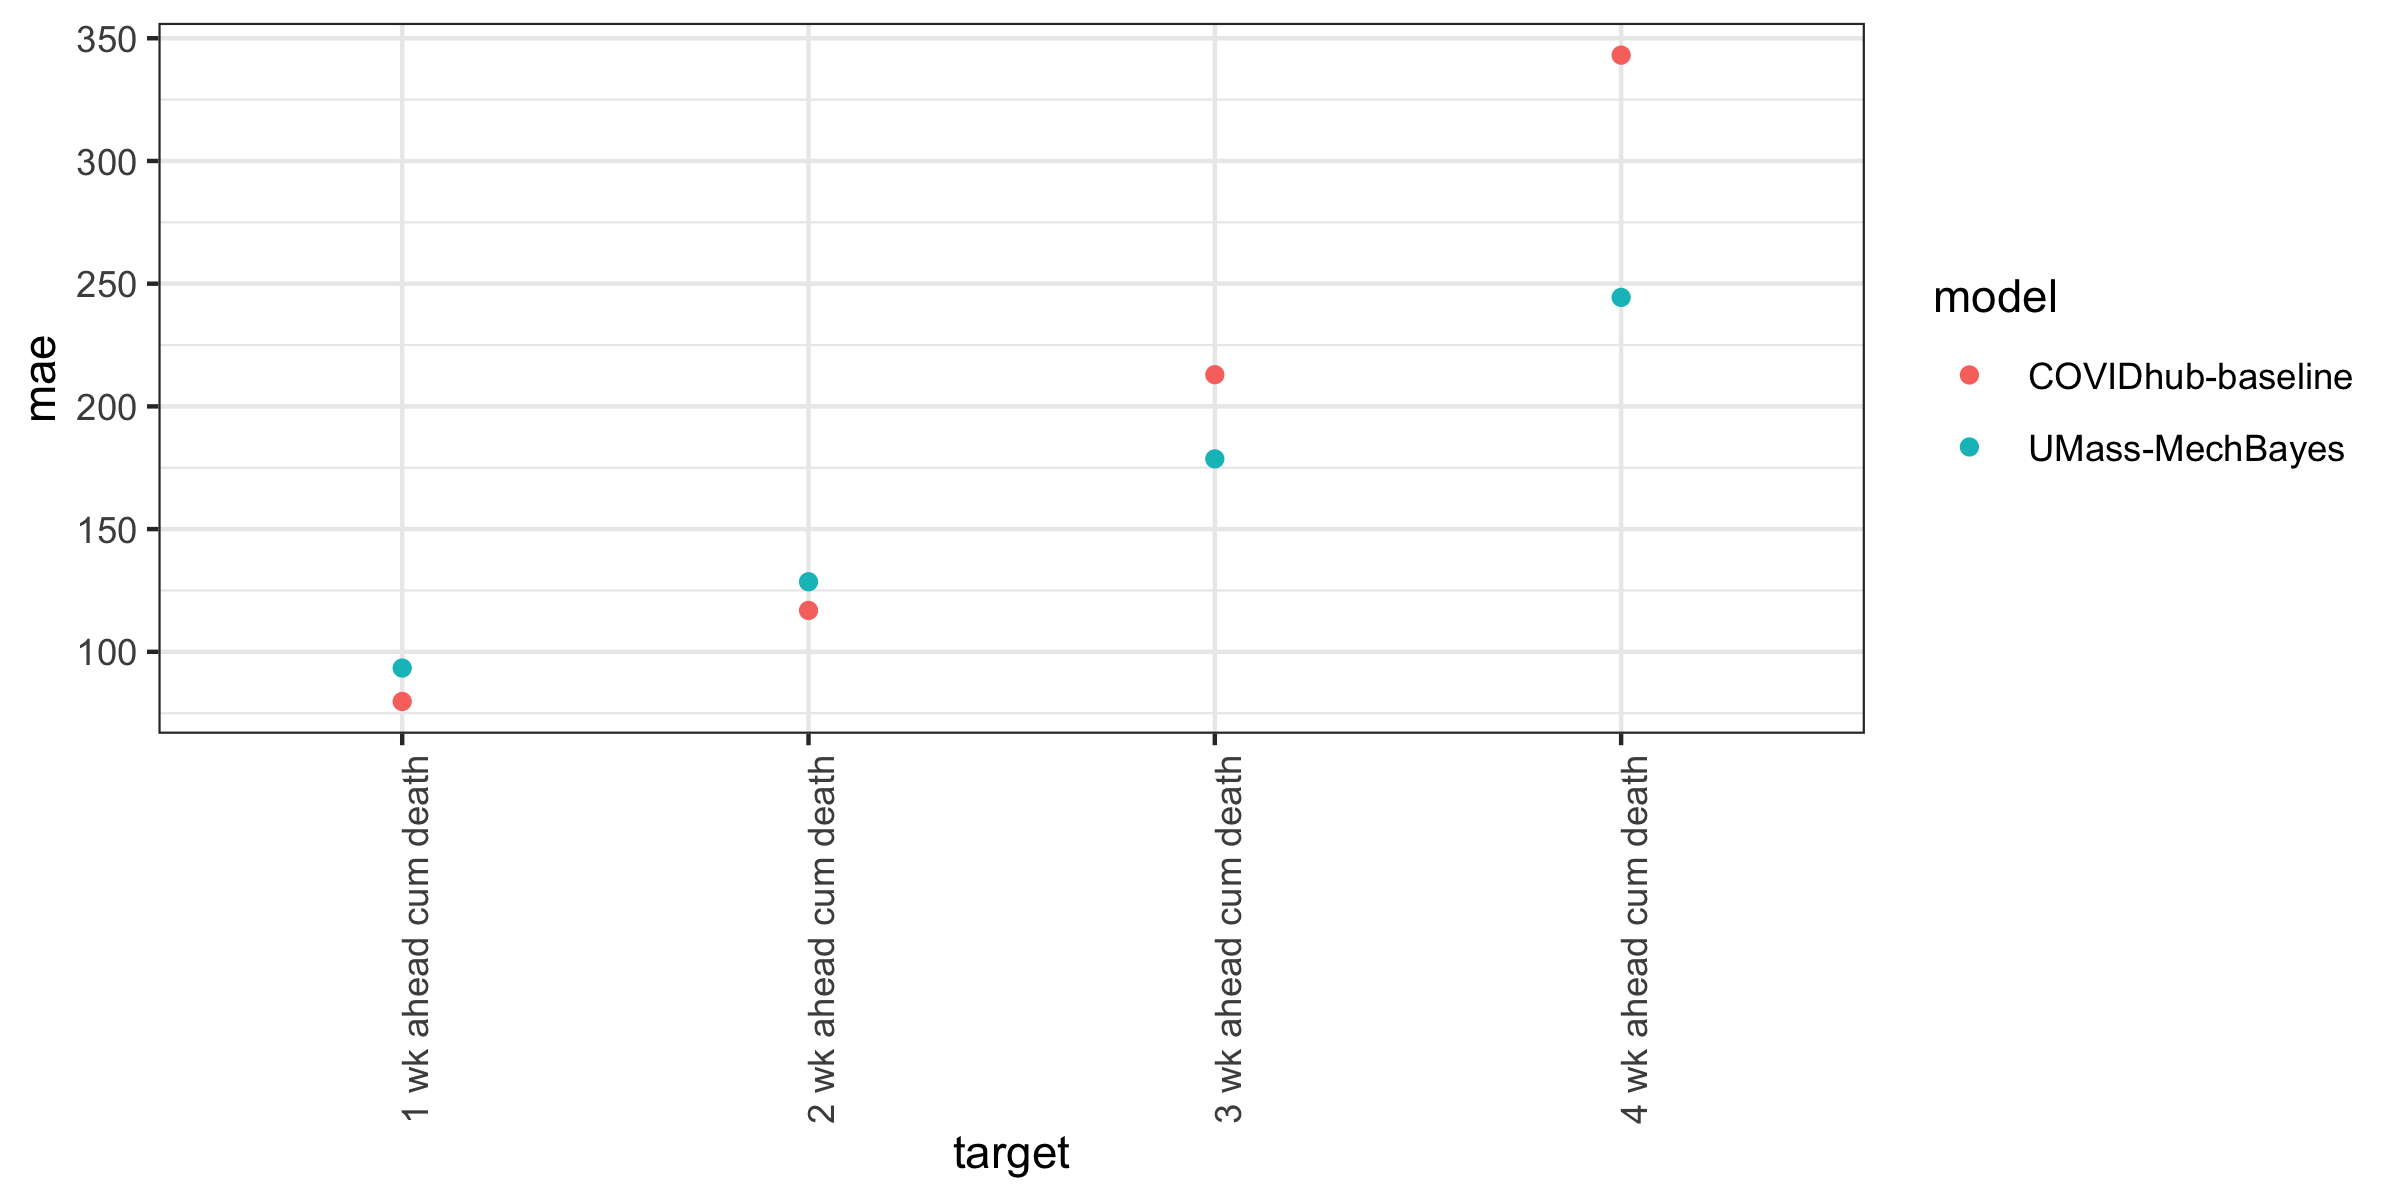
\includegraphics[scale=.1]{mae_results_by_target.png}
%    \caption{MAE by target}
%\end{subfigure}%
%\begin{subfigure}{.5\textwidth}
%  \centering
%    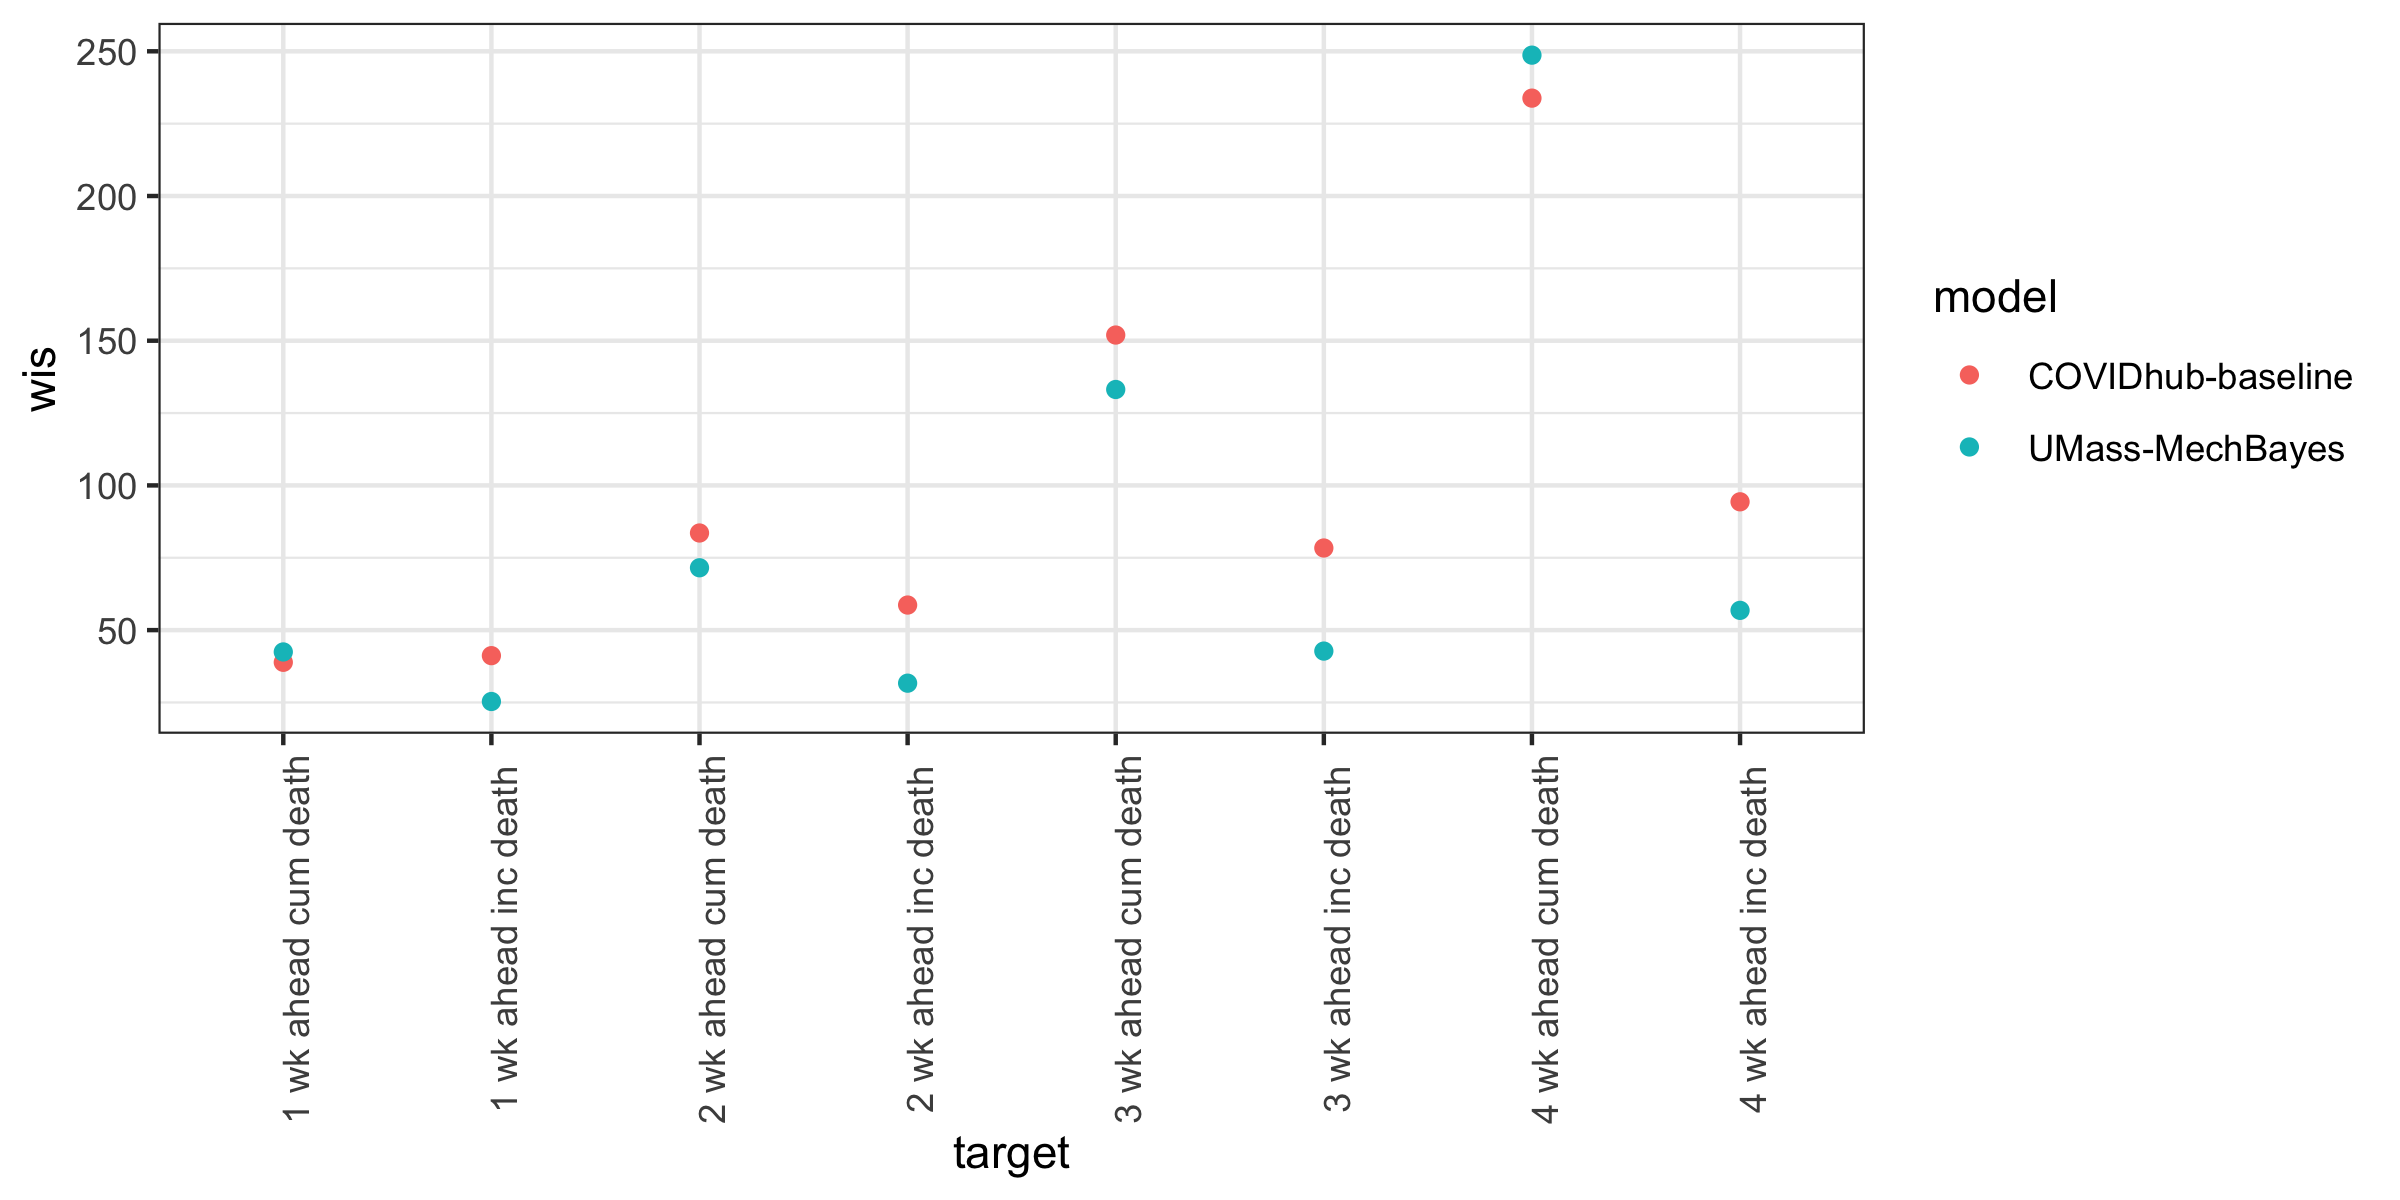
\includegraphics[scale=.1]{wis_results_by_target.png}
%    \caption{WIS by target}
%\end{subfigure}%
%\section{Real-Time Model Results}
%
%\caption{Scores from COVID-19 Forecast Hub broken down by region, target and forecast week. Here we can see that the MechBayes model improves in both MAE and WIS over time, consistently beating the baseline model in the month of July 2020. We can also see that MAE varies heavily by region, which is an artifact of both population size and number of covid deaths. However, in regions with large MAE (left side) we see a significant improvement over the baseline model in terms of both MAE and WIS. Finally, we can see that as the horizon increases from 1 to 4 weeks ahead, both MAE and WIS increase, reflecting an increase in difficulty of forecasting further ahead in time. Note that targets averaging over forecast week include an average over all model versions. }
%\label{fig:covidhub_appendix}
%\end{figure}
%
%
\newpage 


\bibliographystyle{unsrt}
\bibliography{mechbayes}



\end{document}  
